%%%%%%%%%%%%%%%%%%%%%%%%%%%%%%%%%%%%%%%%%%%%%%%%%%%%%%%%%%%%%%%%%%%%%%%%%%%%%%%
% Memorial para concurso público de Professor Doutor na USP.
%
% Formatação inspirada em:
% * https://tug.org/pracjourn/2008-1/mori/mori.pdf
% * https://github.com/santisoler/phd-thesis
% * https://github.com/compgeolab/dissertation-template
%%%%%%%%%%%%%%%%%%%%%%%%%%%%%%%%%%%%%%%%%%%%%%%%%%%%%%%%%%%%%%%%%%%%%%%%%%%%%%%

%%%%%%%%%%%%%%%%%%%%%%%%%%%%%%%%%%%%%%%%%%%%%%%%%%%%%%%%%%%%%%%%%%%%%%%%%%%%%%%
% Set a class and import packages
\documentclass[10pt,a4paper,oneside]{book}

% Variables
\newcommand{\ThesisYear}{2025}
\newcommand{\ThesisAuthor}{Leonardo Uieda}
\newcommand{\ThesisTitle}{Memorial de \ThesisAuthor{} para concurso público - Professor Doutor em Geofísica - IAG/USP}
\newcommand{\ThesisTitleShort}{Tese de Livre Docência}
\newcommand{\ThesisDOI}{XXXXXXXXX}
\newcommand{\Email}{uieda@usp.br}
\newcommand{\ORCID}{0000-0001-6123-9515}

% Import packages
\usepackage[utf8]{inputenc}
\usepackage[T1]{fontenc}
\usepackage[english]{babel}
\usepackage{geometry}
\usepackage{graphicx}
\usepackage{amssymb}
\usepackage{amsmath}
\usepackage{hyperref}
% create fancy headers
\usepackage{fancyhdr}
% commands for managing dates and its formats
\usepackage{datetime2}
% improved urls with proper hyphenation
\usepackage{xurl}
% Control over enumerate and itemize
\usepackage{enumitem}
% Tweak the look of captions
\usepackage{caption}
% To control the style of section titles
\usepackage{titlesec}
% Add the bibliography to the table of contents
\usepackage[nottoc,chapter]{tocbibind}
\usepackage[round,authoryear,sort]{natbib}
% show dois as links on references
\usepackage{doi}
% Icon and fonts (requires using xelatex or luatex)
\usepackage{fontawesome5}
\usepackage{academicons}
\usepackage{fontspec}
\usepackage[mono]{notomath}
% \usepackage{mathpazo}
% \usepackage[sfdefault]{atkinson}
% To make everything neater
\usepackage{microtype}
% To make fancy text boxes
\usepackage{xcolor}
\usepackage[framemethod=default]{mdframed}
% For fancy and multipage tables
\usepackage{tabularx}
\usepackage{ltablex}
% To define custom environments
\usepackage{environ}
\usepackage{setspace}
% Reference sections by name
\usepackage{nameref}
% Better handling of footnotes inside summary boxes
\usepackage{footmisc}
% To create Algorithm floats
\usepackage{algorithm2e}
% To write units in a nice way
\usepackage{siunitx}
% To control what's inside and outside the book parts
\usepackage{bookmark}
%%%%%%%%%%%%%%%%%%%%%%%%%%%%%%%%%%%%%%%%%%%%%%%%%%%%%%%%%%%%%%%%%%%%%%%%%%%%%%%

%%%%%%%%%%%%%%%%%%%%%%%%%%%%%%%%%%%%%%%%%%%%%%%%%%%%%%%%%%%%%%%%%%%%%%%%%%%%%%%
% Mathematical symbols

% Lagrangian
\DeclareMathOperator{\Lagr}{\mathcal{L}}
% Merit function
\DeclareMathOperator{\Merit}{\mathcal{M}}

%%%%%%%%%%%%%%%%%%%%%%%%%%%%%%%%%%%%%%%%%%%%%%%%%%%%%%%%%%%%%%%%%%%%%%%%%%%%%%%
% Configuration of the document

\geometry{%
  left=25mm,
  right=25mm,
  top=20mm,
  bottom=15mm,
  headsep=5mm,
  headheight=5mm,
  footskip=10mm,
  includehead=true,
  includefoot=true
}

% Increase the line spacing
\SetSinglespace{1.2}
\onehalfspacing

% Remove spacing between enumerate/itemize items
\setlist{nosep}

% Make a Unicode bullet symbol
\newcommand{\Bullet}{•\enspace}

% Define custom colors
\definecolor{darkgray}{gray}{0.4}
\definecolor{mediumgray}{gray}{0.5}
\definecolor{lightgray}{gray}{0.9}
\definecolor{mediumblue}{HTML}{2060c2}
\definecolor{lightblue}{HTML}{f7faff}

% Customize how Chapter headings are displayed
\titleformat{\chapter}[display]{\normalfont}{\large Chapter \thechapter}{0pt}{\huge}[\titlerule]
\titlespacing*{\chapter}{0pt}{-40pt}{40pt}

% Set the spacing between bibliography entries (requires natbib)
\setlength{\bibsep}{0pt}

% Configure captions
\captionsetup{labelfont=bf,font={small,color=darkgray},skip=10pt}

% Define fancy text boxes
\NewEnviron{summarybox}{%
  \mdfdefinestyle{summarybox_}{%
    leftline=true,
    rightline=false,
    topline=false,
    bottomline=false,
    linewidth=2pt,
    linecolor=mediumblue,
    backgroundcolor=lightblue,
    innertopmargin=12pt,
    innerbottommargin=12pt,
    innerleftmargin=12pt,
    innerrightmargin=12pt,
    skipbelow=5pt,
    skipabove=5pt,
  }
  \newmdenv[style=summarybox_]{summarybox_}
  \vspace{-0.5cm}
  \begin{summarybox_}
    \footnotesize
    \BODY
  \end{summarybox_}
}

% Configure hyperref and add PDF metadata
\hypersetup{
    colorlinks,
    allcolors=mediumblue,
    pdftitle={\ThesisTitle},
    pdfauthor={\ThesisAuthor},
    pdftex,
    breaklinks=true,
}

% make urls use the same font as every other text
\urlstyle{same}

% Prevent footnotes from being broken into multiple pages
\interfootnotelinepenalty=10000

% Configure headers and footers
\newcommand{\Separator}{\hspace{3pt}|\hspace{3pt}}
\newcommand{\HeaderFont}{\footnotesize\color{mediumgray}}
\preto{\footrule}{\color{lightgray}}
\fancyhf{}
\lhead{%
    \HeaderFont{}
    \nouppercase\leftmark{}
    \Separator{}
    \ThesisTitleShort{}
}
\chead{}
\rhead{%
    \HeaderFont{}
    \ThesisAuthor{}
    \Separator{}
    \thepage\space de\space \pageref*{LastPage}
}
\cfoot{}
\renewcommand{\headrulewidth}{0.3pt}
%%%%%%%%%%%%%%%%%%%%%%%%%%%%%%%%%%%%%%%%%%%%%%%%%%%%%%%%%%%%%%%%%%%%%%%%%%%%%%%

%%%%%%%%%%%%%%%%%%%%%%%%%%%%%%%%%%%%%%%%%%%%%%%%%%%%%%%%%%%%%%%%%%%%%%%%%%%%%%%
\begin{document}

\pagestyle{plain}
\frontmatter

\begin{titlepage}
  \begin{center}
    
\includegraphics[height=1.5cm]{images/usp.png}
    \hspace{1cm}
    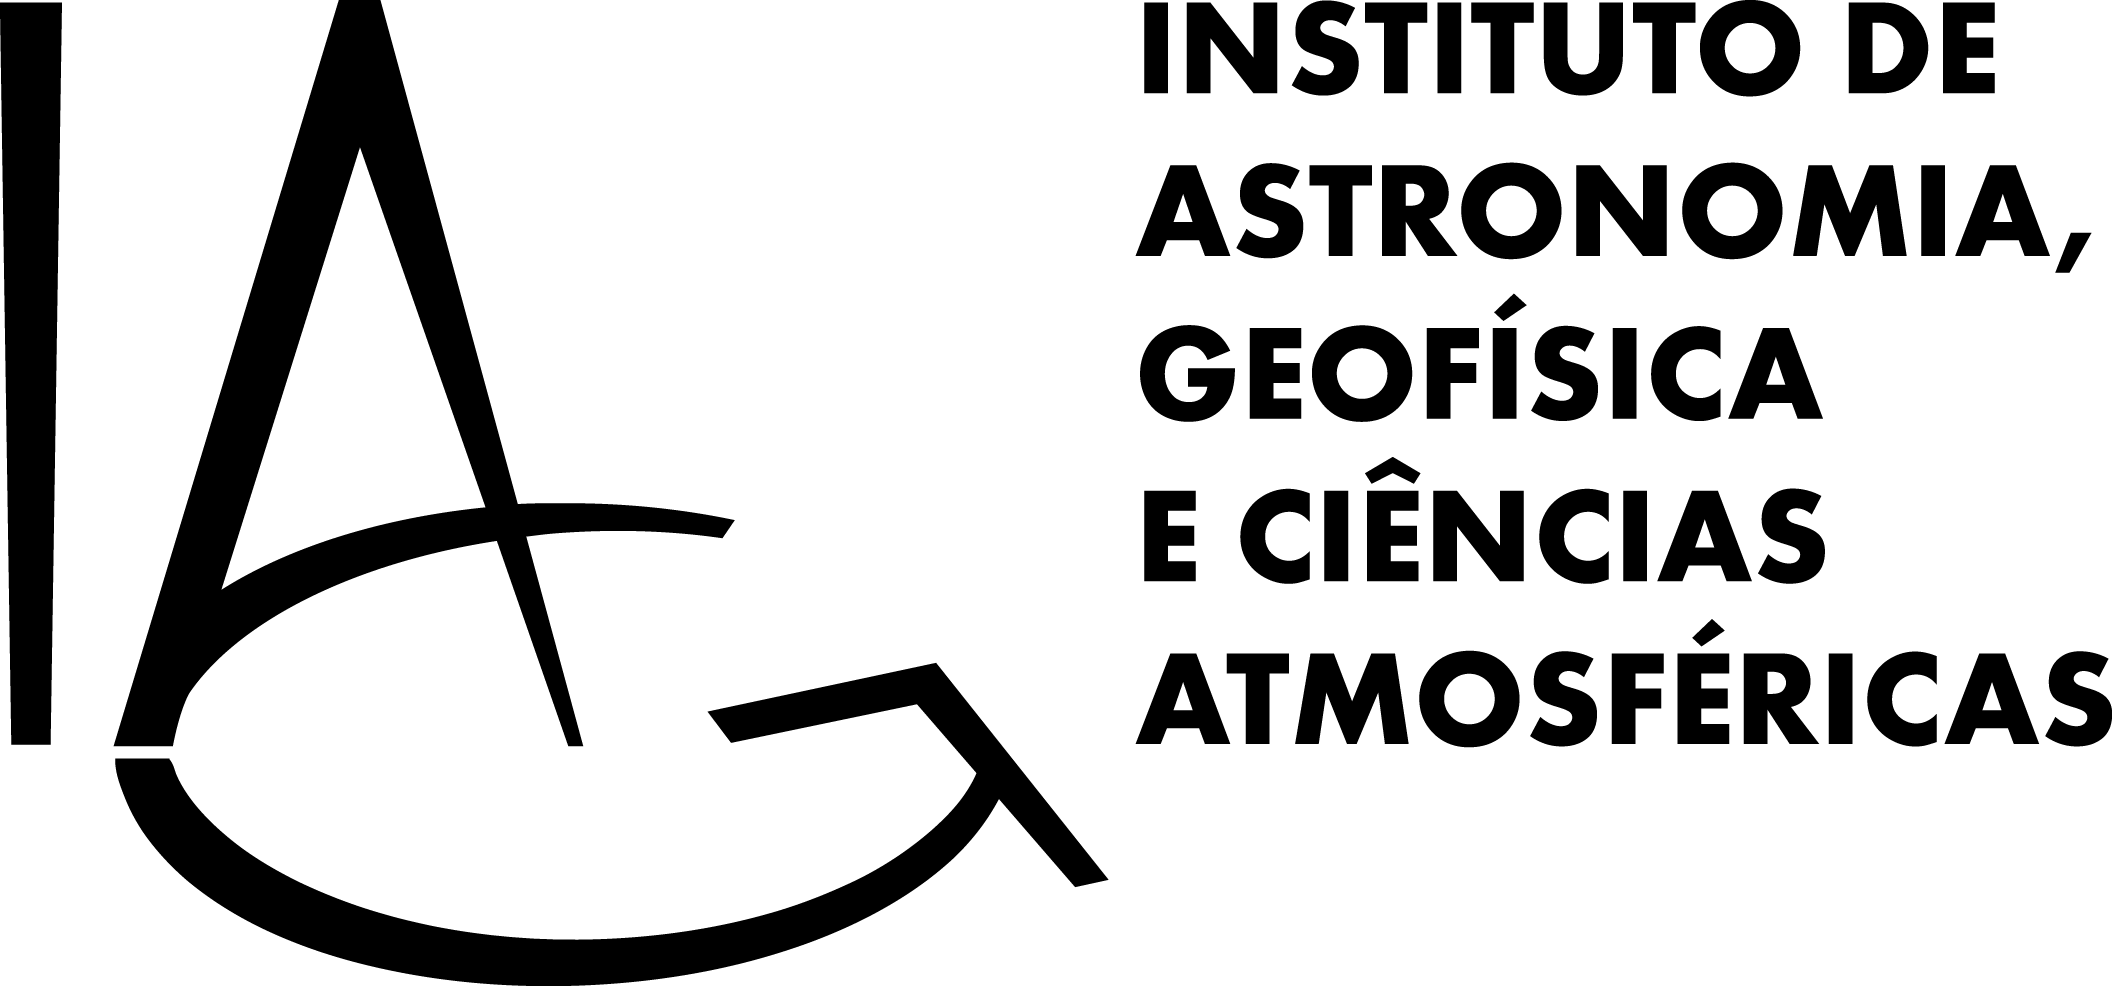
\includegraphics[height=1.5cm]{images/iag.png}
    \vspace{1cm}

    UNIVERSIDADE DE SÃO PAULO

    INSTITUTO DE ASTRONOMIA, GEOFÍSICA E CIÊNCIAS ATMOSFÉRICAS
    \vspace{5cm}

    \textbf{\huge \ThesisTitle}
    \vspace{2cm}

    {\Large \ThesisAuthor}
    \vspace{5cm}

    {\small
      Tese apresentada para concurso títulos e provas visando a obtenção do

      título de Livre Docente junto ao Departamento de Geofísica do

      Instituto de Astronomia, Geofísica e Ciências Atmosféricas da

      Universidade de São Paulo.
      \vspace{1cm}

      Edital ATAc-IAG/005/2025
    }
    \vfill

    \ThesisYear{}
  \end{center}
\end{titlepage}


%==============================================================================

{\small

\vspace*{\fill}

\noindent
\textit{\ThesisTitle{}}.
\\[0.2cm]
\textcopyright{} Copyright \ThesisYear{} \ThesisAuthor{} (ORCID:
\href{https://orcid.org/\ORCID}{\ORCID}).
\\[0.2cm]
Última modificação em \today.
doi:\href{https://doi.org/\ThesisDOI}{\ThesisDOI}.

\vspace{2.5cm}

\noindent
\textbf{\LARGE \faCreativeCommons{} \faCreativeCommonsBy{}}
\\
Disponível sob a
\textbf{Licença Creative Commons Atribuição 4.0 Internacional}.
\\
\url{https://creativecommons.org/licenses/by/4.0/deed.pt-br}

\vspace{0.25cm}

\noindent
Você tem o direito de:

\begin{description}[labelindent=0.5cm]
    \item[Compartilhar ---]{
        Copiar e redistribuir o material em qualquer suporte ou formato para
        qualquer fim, mesmo que comercial.
    }
    \item[Adaptar ---]{
        Remixar, transformar, e criar a partir do material para qualquer fim,
        mesmo que comercial.
    }
\end{description}

\vspace{0.25cm}

\noindent
De acordo com os termos seguintes:

\begin{description}[labelindent=0.5cm]
    \item[Atribuição ---]{
         Você deve dar o crédito apropriado, prover um link para a licença
         e indicar se mudanças foram feitas. Você deve fazê-lo em qualquer
         circunstância razoável, mas de nenhuma maneira que sugira que
         o licenciante apoia você ou o seu uso.
    }
    \item[Sem restrições adicionais ---]{
        Você não pode aplicar termos jurídicos ou medidas de caráter
        tecnológico que restrinjam legalmente outros de fazerem algo que
        a licença permita.
}
\end{description}

\vspace{1.5cm}

}

%==============================================================================
\chapter*{Abstract}

Bla.

%==============================================================================
\tableofcontents

\mainmatter
\pagestyle{fancy}

%==============================================================================
\chapter{Introduction}

Bla.

%==============================================================================
\chapter{Gradient-boosted equivalent sources}

\begingroup
% Title, authors and affiliations
\newcommand{\Title}{Gradient-boosted equivalent sources}
\newcommand{\Soler}{Santiago R. Soler}
\newcommand{\SolerShort}{Soler}
\newcommand{\SolerMail}{santiago.r.soler@gmail.com}
\newcommand{\SolerORCID}{0000-0001-9202-5317}
\newcommand{\Uieda}{Leonardo Uieda}
\newcommand{\UiedaShort}{Uieda}
\newcommand{\UiedaORCID}{0000-0001-6123-9515}
\newcommand{\CONICET}{%
    Consejo Nacional de Investigaciones Científicas y Técnicas (CONICET),
    Ciudad Autónoma de Buenos Aires, Argentina
}
\newcommand{\IGSV}{%
    Instituto Geofísico Sismológico Volponi,
    Universidad Nacional de San Juan, San Juan, Argentina
}
\newcommand{\Liverpool}{%
    Department of Earth, Ocean and Ecological Sciences, School of Environmental
    Sciences, University of Liverpool, UK
}

% Publication-related variables
\newcommand{\Journal}{Geophysical Journal International}
\newcommand{\Year}{2021}

% DOIs
\newcommand{\PreprintDOI}{10.31223/X58G7C}
\newcommand{\DOI}{10.1093/gji/ggab297}
\newcommand{\DOILink}{\href{https://doi.org/\DOI}{doi.org/\DOI}}


% Keywords for GJI
\newcommand{\keywordsGJI}{%
Gravity anomalies and Earth structure;
Magnetic anomalies: modelling and interpretation;
Geopotential theory;
Inverse theory;
Statistical methods;
Australia.
}

% Define inverse symbol with shorter minus
\newcommand{\inv}{^{\text{-}1}}
\newcommand{\trans}{^{\text{T}}}

% Define some units
\renewcommand{\m}{$\,$m}
\renewcommand{\km}{$\,$km}
\newcommand{\mGal}{$\,$mGal}

% Import files with parameter values generated by notebooks
\newcommand{\NPrisms}{64}
\newcommand{\ModelEasting}{$111319 \, \text{m}$}
\newcommand{\ModelNorthing}{$111319 \, \text{m}$}
\newcommand{\ModelDepth}{$10000 \, \text{m}$}
\newcommand{\ModelMinDensity}{$-900 \, \text{kg} \, \text{m}^{-3}$}
\newcommand{\ModelMaxDensity}{$500 \, \text{kg} \, \text{m}^{-3}$}
\newcommand{\SurveyEasting}{$111319 \, \text{m}$}
\newcommand{\SurveyNorthing}{$110576 \, \text{m}$}
\newcommand{\SurveyNoise}{$1 \, \text{mGal}$}
\newcommand{\GroundSurveyPoints}{963}
\newcommand{\GroundSurveyMinHeight}{$0 \, \text{m}$}
\newcommand{\GroundSurveyMaxHeight}{$2052.2 \, \text{m}$}
\newcommand{\AirborneSurveyPoints}{5673}
\newcommand{\AirborneSurveyMinHeight}{$359 \, \text{m}$}
\newcommand{\AirborneSurveyMaxHeight}{$1255 \, \text{m}$}
\newcommand{\TargetHeight}{$2000 \, \text{m}$}
\newcommand{\TargetSpacing}{$2 \, \text{km}$}
\newcommand{\TargetEastingSize}{57}
\newcommand{\TargetNorthingSize}{56}
\newcommand{\GroundSourceBelowDataConstantDepthDamping}{10$^{-4}$, 10$^{-3}$,$\dots$, 10$^{2}$}
\newcommand{\GroundSourceBelowDataConstantDepthDepth}{1000 to 17000, step size 2000}
\newcommand{\GroundSourceBelowDataRelativeDepthDamping}{10$^{-4}$, 10$^{-3}$,$\dots$, 10$^{2}$}
\newcommand{\GroundSourceBelowDataRelativeDepthDepth}{1000 to 17000, step size 2000}
\newcommand{\GroundSourceBelowDataVariableDepthDamping}{10$^{-4}$, 10$^{-3}$,$\dots$, 10$^{2}$}
\newcommand{\GroundSourceBelowDataVariableDepthDepthFactor}{0.1, 0.5, 1, 2, 3, 4, 5 and 6}
\newcommand{\GroundSourceBelowDataVariableDepthDepth}{0 to 1400, step size 200}
\newcommand{\GroundSourceBelowDataVariableDepthKNearest}{1, 5, 10 and 15}
\newcommand{\GroundBlockAveragedSourcesConstantDepthDamping}{10$^{-4}$, 10$^{-3}$,$\dots$, 10$^{2}$}
\newcommand{\GroundBlockAveragedSourcesConstantDepthDepth}{1000 to 17000, step size 2000}
\newcommand{\GroundBlockAveragedSourcesConstantDepthSpacing}{1000, 2000, 3000 and 4000}
\newcommand{\GroundBlockAveragedSourcesRelativeDepthDamping}{10$^{-4}$, 10$^{-3}$,$\dots$, 10$^{2}$}
\newcommand{\GroundBlockAveragedSourcesRelativeDepthDepth}{1000 to 17000, step size 2000}
\newcommand{\GroundBlockAveragedSourcesRelativeDepthSpacing}{1000, 2000, 3000 and 4000}
\newcommand{\GroundBlockAveragedSourcesVariableDepthDamping}{10$^{-4}$, 10$^{-3}$,$\dots$, 10$^{2}$}
\newcommand{\GroundBlockAveragedSourcesVariableDepthSpacing}{1000, 2000, 3000 and 4000}
\newcommand{\GroundBlockAveragedSourcesVariableDepthDepthFactor}{0.1, 0.5, 1, 2, 3, 4, 5 and 6}
\newcommand{\GroundBlockAveragedSourcesVariableDepthDepth}{0 to 1400, step size 200}
\newcommand{\GroundBlockAveragedSourcesVariableDepthKNearest}{1, 5, 10 and 15}
\newcommand{\GroundGridSourcesConstantDepthDamping}{10$^{1}$, 10$^{2}$, 10$^{3}$ and 10$^{4}$}
\newcommand{\GroundGridSourcesConstantDepthDepth}{1000 to 9000, step size 2000}
\newcommand{\GroundGridSourcesConstantDepthSpacing}{1000, 2000, 3000 and 4000}
\newcommand{\AirborneSourceBelowDataConstantDepthDamping}{10$^{-4}$, 10$^{-3}$,$\dots$, 10$^{2}$}
\newcommand{\AirborneSourceBelowDataConstantDepthDepth}{1000 to 17000, step size 2000}
\newcommand{\AirborneSourceBelowDataRelativeDepthDamping}{10$^{-4}$, 10$^{-3}$,$\dots$, 10$^{2}$}
\newcommand{\AirborneSourceBelowDataRelativeDepthDepth}{1000 to 17000, step size 2000}
\newcommand{\AirborneSourceBelowDataVariableDepthDamping}{10$^{-4}$, 10$^{-3}$,$\dots$, 10$^{2}$}
\newcommand{\AirborneSourceBelowDataVariableDepthDepthFactor}{1 to 6, step size 1}
\newcommand{\AirborneSourceBelowDataVariableDepthDepth}{50 to 1450, step size 200}
\newcommand{\AirborneSourceBelowDataVariableDepthKNearest}{1, 5, 10 and 15}
\newcommand{\AirborneBlockAveragedSourcesConstantDepthDamping}{10$^{-4}$, 10$^{-3}$,$\dots$, 10$^{2}$}
\newcommand{\AirborneBlockAveragedSourcesConstantDepthDepth}{1000 to 17000, step size 2000}
\newcommand{\AirborneBlockAveragedSourcesConstantDepthSpacing}{1000, 2000, 3000 and 4000}
\newcommand{\AirborneBlockAveragedSourcesRelativeDepthDamping}{10$^{-4}$, 10$^{-3}$,$\dots$, 10$^{2}$}
\newcommand{\AirborneBlockAveragedSourcesRelativeDepthDepth}{1000 to 17000, step size 2000}
\newcommand{\AirborneBlockAveragedSourcesRelativeDepthSpacing}{1000, 2000, 3000 and 4000}
\newcommand{\AirborneBlockAveragedSourcesVariableDepthDamping}{10$^{-4}$, 10$^{-3}$,$\dots$, 10$^{2}$}
\newcommand{\AirborneBlockAveragedSourcesVariableDepthSpacing}{1000, 2000, 3000 and 4000}
\newcommand{\AirborneBlockAveragedSourcesVariableDepthDepthFactor}{1 to 6, step size 1}
\newcommand{\AirborneBlockAveragedSourcesVariableDepthDepth}{50 to 1450, step size 200}
\newcommand{\AirborneBlockAveragedSourcesVariableDepthKNearest}{1, 5, 10 and 15}
\newcommand{\AirborneGridSourcesConstantDepthDamping}{10$^{-3}$, 10$^{-2}$,$\dots$, 10$^{2}$}
\newcommand{\AirborneGridSourcesConstantDepthDepth}{1000 to 9000, step size 2000}
\newcommand{\AirborneGridSourcesConstantDepthSpacing}{1000, 2000 and 3000}
\newcommand{\BestGroundSourceBelowDataConstantDepthDamping}{10$^{-1}$}
\newcommand{\BestGroundSourceBelowDataConstantDepthDepth}{7000}
\newcommand{\BestGroundSourceBelowDataConstantDepthRms}{0.78}
\newcommand{\BestGroundSourceBelowDataConstantDepthNPoints}{963}
\newcommand{\BestGroundSourceBelowDataRelativeDepthDamping}{10$^{-1}$}
\newcommand{\BestGroundSourceBelowDataRelativeDepthDepth}{9000}
\newcommand{\BestGroundSourceBelowDataRelativeDepthRms}{0.79}
\newcommand{\BestGroundSourceBelowDataRelativeDepthNPoints}{963}
\newcommand{\BestGroundSourceBelowDataVariableDepthDamping}{1}
\newcommand{\BestGroundSourceBelowDataVariableDepthDepthFactor}{1}
\newcommand{\BestGroundSourceBelowDataVariableDepthDepth}{1000}
\newcommand{\BestGroundSourceBelowDataVariableDepthKNearest}{15}
\newcommand{\BestGroundSourceBelowDataVariableDepthRms}{0.80}
\newcommand{\BestGroundSourceBelowDataVariableDepthNPoints}{963}
\newcommand{\BestGroundBlockAveragedSourcesConstantDepthDamping}{10$^{-1}$}
\newcommand{\BestGroundBlockAveragedSourcesConstantDepthDepth}{7000}
\newcommand{\BestGroundBlockAveragedSourcesConstantDepthSpacing}{3000}
\newcommand{\BestGroundBlockAveragedSourcesConstantDepthRms}{0.77}
\newcommand{\BestGroundBlockAveragedSourcesConstantDepthNPoints}{518}
\newcommand{\BestGroundBlockAveragedSourcesRelativeDepthDamping}{10$^{-1}$}
\newcommand{\BestGroundBlockAveragedSourcesRelativeDepthDepth}{7000}
\newcommand{\BestGroundBlockAveragedSourcesRelativeDepthSpacing}{3000}
\newcommand{\BestGroundBlockAveragedSourcesRelativeDepthRms}{0.79}
\newcommand{\BestGroundBlockAveragedSourcesRelativeDepthNPoints}{518}
\newcommand{\BestGroundBlockAveragedSourcesVariableDepthDamping}{10$^{-1}$}
\newcommand{\BestGroundBlockAveragedSourcesVariableDepthSpacing}{3000}
\newcommand{\BestGroundBlockAveragedSourcesVariableDepthDepthFactor}{1}
\newcommand{\BestGroundBlockAveragedSourcesVariableDepthDepth}{600}
\newcommand{\BestGroundBlockAveragedSourcesVariableDepthKNearest}{15}
\newcommand{\BestGroundBlockAveragedSourcesVariableDepthRms}{0.72}
\newcommand{\BestGroundBlockAveragedSourcesVariableDepthNPoints}{518}
\newcommand{\BestGroundGridSourcesConstantDepthDamping}{10$^{2}$}
\newcommand{\BestGroundGridSourcesConstantDepthDepth}{3000}
\newcommand{\BestGroundGridSourcesConstantDepthSpacing}{2000}
\newcommand{\BestGroundGridSourcesConstantDepthRms}{0.97}
\newcommand{\BestGroundGridSourcesConstantDepthNPoints}{3192}
\newcommand{\BestAirborneSourceBelowDataConstantDepthDamping}{10$^{-2}$}
\newcommand{\BestAirborneSourceBelowDataConstantDepthDepth}{7000}
\newcommand{\BestAirborneSourceBelowDataConstantDepthRms}{0.35}
\newcommand{\BestAirborneSourceBelowDataConstantDepthNPoints}{5673}
\newcommand{\BestAirborneSourceBelowDataRelativeDepthDamping}{10$^{-2}$}
\newcommand{\BestAirborneSourceBelowDataRelativeDepthDepth}{9000}
\newcommand{\BestAirborneSourceBelowDataRelativeDepthRms}{0.35}
\newcommand{\BestAirborneSourceBelowDataRelativeDepthNPoints}{5673}
\newcommand{\BestAirborneSourceBelowDataVariableDepthDamping}{1}
\newcommand{\BestAirborneSourceBelowDataVariableDepthDepthFactor}{1}
\newcommand{\BestAirborneSourceBelowDataVariableDepthDepth}{1450}
\newcommand{\BestAirborneSourceBelowDataVariableDepthKNearest}{15}
\newcommand{\BestAirborneSourceBelowDataVariableDepthRms}{0.36}
\newcommand{\BestAirborneSourceBelowDataVariableDepthNPoints}{5673}
\newcommand{\BestAirborneBlockAveragedSourcesConstantDepthDamping}{10$^{-4}$}
\newcommand{\BestAirborneBlockAveragedSourcesConstantDepthDepth}{9000}
\newcommand{\BestAirborneBlockAveragedSourcesConstantDepthSpacing}{3000}
\newcommand{\BestAirborneBlockAveragedSourcesConstantDepthRms}{0.34}
\newcommand{\BestAirborneBlockAveragedSourcesConstantDepthNPoints}{1100}
\newcommand{\BestAirborneBlockAveragedSourcesRelativeDepthDamping}{10$^{-3}$}
\newcommand{\BestAirborneBlockAveragedSourcesRelativeDepthDepth}{9000}
\newcommand{\BestAirborneBlockAveragedSourcesRelativeDepthSpacing}{2000}
\newcommand{\BestAirborneBlockAveragedSourcesRelativeDepthRms}{0.34}
\newcommand{\BestAirborneBlockAveragedSourcesRelativeDepthNPoints}{1663}
\newcommand{\BestAirborneBlockAveragedSourcesVariableDepthDamping}{10$^{-2}$}
\newcommand{\BestAirborneBlockAveragedSourcesVariableDepthSpacing}{2000}
\newcommand{\BestAirborneBlockAveragedSourcesVariableDepthDepthFactor}{2}
\newcommand{\BestAirborneBlockAveragedSourcesVariableDepthDepth}{50}
\newcommand{\BestAirborneBlockAveragedSourcesVariableDepthKNearest}{15}
\newcommand{\BestAirborneBlockAveragedSourcesVariableDepthRms}{0.33}
\newcommand{\BestAirborneBlockAveragedSourcesVariableDepthNPoints}{1663}
\newcommand{\BestAirborneGridSourcesConstantDepthDamping}{10$^{-1}$}
\newcommand{\BestAirborneGridSourcesConstantDepthDepth}{7000}
\newcommand{\BestAirborneGridSourcesConstantDepthSpacing}{1000}
\newcommand{\BestAirborneGridSourcesConstantDepthRms}{0.34}
\newcommand{\BestAirborneGridSourcesConstantDepthNPoints}{12544}
\newcommand{\SourceLayoutsSchematicsObservations}{166}
\newcommand{\SourceLayoutsSchematicsSourceBelowData}{166}
\newcommand{\SourceLayoutsSchematicsGridSources}{378}
\newcommand{\SourceLayoutsSchematicsBlockAveragedSources}{87}
\newcommand{\BoostOverlappingWindowSize}{$30000 \, \text{m}$}
\newcommand{\EqlBoostAirborneRmsScore}{$0.38 \, \text{mGal}$}
\newcommand{\EqlBoostAirborneDepth}{$3000 \, \text{m}$}
\newcommand{\EqlBoostAirborneDamping}{0.1}
\newcommand{\EqlBoostAirborneSpacing}{$2 \, \text{km}$}
\newcommand{\EqlBoostAirborneWindowSize}{$20 \, \text{km}$}
\newcommand{\EqlBoostAirborneNSources}{1663}
\newcommand{\EqlBoostAirborneMinDepth}{$1000 \, \text{m}$}
\newcommand{\EqlBoostAirborneMaxDepth}{$19000 \, \text{m}$}
\newcommand{\EqlBoostAirborneMinDamping}{1e-06}
\newcommand{\EqlBoostAirborneMaxDamping}{10}
\newcommand{\AustraliaSmallAreaEastingSize}{$300 \, \text{km}$}
\newcommand{\AustraliaSmallAreaNorthingSize}{$300 \, \text{km}$}
\newcommand{\AustraliaSmallAreaNPoints}{14934}
\newcommand{\AustraliaDepthMin}{$1000 \, \text{m}$}
\newcommand{\AustraliaDepthMax}{$15000 \, \text{m}$}
\newcommand{\AustraliaDampingMin}{0.01}
\newcommand{\AustraliaDampingMax}{10000}
\newcommand{\AustraliaEqlDepth}{$3000 \, \text{m}$}
\newcommand{\AustraliaEqlDamping}{100}
\newcommand{\AustraliaEqlSpacing}{$1800 \, \text{m}$}
\newcommand{\AustraliaEqlWindowSize}{$225 \, \text{km}$}
\newcommand{\AustraliaEqlRmsScore}{$1.33 \, \text{mGal}$}
\newcommand{\AustraliaEqlNSources}{796744}
\newcommand{\AustraliaEqlGridNLongitude}{2442}
\newcommand{\AustraliaEqlGridNLatitude}{2085}
\newcommand{\AustraliaEqlGridHeight}{$2127.58 \, \text{m}$}



\begin{summarybox}
    \noindent
    This chapter was originally published as
    \textbf{``Soler, S. R. and Uieda, L. (\Year). \Title{}. \textit{\Journal{}}.
    doi:\href{https://doi.org/\DOI}{\DOI}.''}, which was previously published
    as a preprint on EarthArXiv (\url{https://doi.org/\PreprintDOI}) under the
    terms of the CC-BY license. It is reproduced here under these terms.
\end{summarybox}

\section*{Abstract}
The equivalent source technique is a powerful and widely used method for
processing gravity and magnetic data.  Nevertheless, its major
drawback is the large computational cost in terms of processing time and
computer memory.
We present two techniques for reducing the computational cost of equivalent
source processing: block-averaging source locations and the
gradient-boosted equivalent source algorithm.
Through block-averaging, we reduce the number of source coefficients that
must be estimated while retaining the minimum desired resolution in the final
processed data.
With the gradient boosting method, we estimate the sources coefficients in
small batches along overlapping windows, allowing us to reduce the computer
memory requirements arbitrarily to conform to the constraints of the
available hardware.
We show that the combination of block-averaging and gradient-boosted
equivalent sources is capable of producing accurate interpolations through
tests against synthetic data.
Moreover, we demonstrate the feasibility of our method by gridding a gravity
dataset covering Australia with over 1.7 million observations using a modest
personal computer.


% \section{Introduction}

Measurements of anomalies in potential fields, like gravity disturbances and
total-field magnetic anomalies, are widely used in geophysical exploration for
their low cost of acquisition.
These data can be surveyed using ground, airborne, shipborne, or satellite
systems.
During ground surveys, the data are often gathered following irregular paths or
networks along the surface of the terrain, leading to highly variable
elevations in mountainous regions.
Airborne and satellite surveys gather data along flight lines, producing
closely spaced measurements along almost straight lines but with larger spacing
between adjacent lines.
Measurement height can also change because of the vertical movement of the
aircraft.
Processing of the data often involves interpolation onto a regular grid at
constant height, both to improve visualization for interpretation purposes as
well as to prepare the data for further processing and modelling (e.g.,
reduction-to-the-pole, derivative calculations, upward continuation, Euler
deconvolution).

Several methods exist in the literature for interpolation in two dimensions,
for example continuous curvature splines in tension \citep{smith1990},
bi-harmonic (thin-plate) splines \citep{sandwell1987}, and kriging
\citep{hansen1993}.
These general-purpose methods have limitations when it comes to interpolating
potential field data, namely
(i)~they are not able to take into account the variable height of the
observation points and
(ii)~the interpolating functions are not necessarily harmonic, which
is the underlying assumption behind many processing techniques
(e.g., upward continuation and vertical derivatives).

A widely used method for interpolating gravity and magnetic data
is the equivalent sources technique (also known as equivalent layer, radial
basis functions, or Green's functions interpolation).
First introduced by \citet{dampney1969}, the method consists in fitting a model
of finite elementary sources to the data and using this model to predict new
data values.
Besides interpolation, equivalent sources have been used for
reduction-to-the-pole of magnetic data
\citep{silva1986, nakatsuka2006, Guspi2009}, upward
continuation \citep{emilia1973, Li2010}, joint processing of gravity gradient
data \citep{barnes2011}, modelling the lithospheric magnetic field
\citep{kother2015}, recovering the magnetic induction vector from
total-field magnetic anomalies \citep{li2020}, and more.

It is also worth mentioning the least-squares collocation method
(LSC), which is widely used in geodesy
\citep[][and references therein]{tscherning2015}.
LCS is often applied to combine and interpolate different linear functionals of
the disturbing gravity potential (gravity anomalies, gravity disturbances,
deflections of the vertical, geoid height, et cetera).
Like equivalent sources, collocation also requires the solution of a large
linear system of the order of the number of observed data.
As such, it's practical application suffers from the same computational
challenges.

Many variants of the equivalent sources technique have been proposed, often
attempting to obtain faster or more accurate solutions.
The key factors that vary between them are: (i) the type of source, (ii)
the location of the sources, and (iii) the solution strategy.

The most commonly used type of source is a point mass for gravity or dipole for
magnetics \citep[e.g.,~][]{vonfrese1981, silva1986, Mendona1994,
Siqueira2017}.
However, right-rectangular prisms \citep[e.g.,][]{barnes2011, Jirigalatu2019,
li2020} and tesseroids \citep{bouman2016} have also been used successfully.
In fact, even point sources with a simple inverse distance function, instead of
actual gravity or magnetic fields, can be used as
equivalent sources \citep{cordell1992}.

The location of sources often follows one of two strategies.
The most common approach is to distribute sources on a regular grid at a
constant depth \citep[e.g.,~][]{Leao1989, barnes2011, OliveiraJr2013}.
Alternatively, sources can be placed beneath each data point
\citep[e.g.,~][]{cordell1992, Siqueira2017}.
Some recent work by \citet{li2020} places the sources in two overlapping layers
at different depths.

The coefficients of the equivalent source model are often estimated through
damped least-squares.
This imposes a heavy computational load when the number of data points is
large (e.g., airborne and satellite surveys).
To reduce the computational load, \citet{Mendona1994} built the solution
iteratively by incorporating one data point at a time using the ``equivalent
data concept''.
\citet{Leao1989} processed the input data using a moving window, only fitting the
data inside the window and predicting observations at its center.
\citet{Li2010} and \citet{barnes2011} apply different operations to generate a
sparse representation of the sensitive matrix (respectively, wavelet
compression and quadtree discretization), which significantly improves the
speed of the least-squares solution.
\citet{OliveiraJr2013} parametrized the equivalent layer as a piecewise bivariate
polynomial function, reducing the number of parameters in the solution.
\citet{Siqueira2017} developed an iterative solution in which the sensitivity
matrix is transformed into a diagonal matrix with constant terms through the
``excess mass criterion''.
\citet{Jirigalatu2019} applied the Gauss-FFT method to speed up the forward
modelling operations and solved the least-squares problem using steepest
descent to avoid calculating the Hessian matrix and solving linear systems.

Many of the existing methods solve under-determined problems, requiring a much
larger number of equivalent sources than the number of data points.
Some achieve greater efficiency by restricting their applications
to specific data types \citep{Siqueira2017},
interpolating only on regular grids \citep{Leao1989},
or requiring already gridded data \citep{takahashi2020},
to name a few.
Furthermore, many of the optimizations proposed are also complex to implement
in a computer program, limiting their wider adoption.

In the present study,
we propose two strategies for reducing the computational load of
the equivalent sources technique:

\begin{enumerate}
    \item Reduce the number of equivalent sources for oversampled surveys
      through a \emph{block-averaging} strategy while maintaining the quality
      of the solution.
    \item Fit the equivalent source model iteratively along overlapping windows
      using a \emph{gradient boosting} algorithm \citep{friedman2001}.
\end{enumerate}

The first strategy consists in dividing the survey area into horizontal blocks
and assigning a single source to each block, located at the median horizontal
location of the data points.
For airborne, shipborne, and satellite surveys, which are oversampled along
tracks, this can greatly reduce the size of the inverse problem while retaining
the same quality of interpolation.

The gradient boosting algorithm allows us to fit the equivalent source model
iteratively by operating on individual overlapping windows.
As a result, our method solves several much smaller least-squares problems
instead of a large one.
This has some similarities with the strategy used by \citet{Leao1989} but
without the requirement for sources and predictions to be on regular grids.

Through tests on synthetic data, we show that:
(i)~the \emph{block-averaged} sources are able to achieve the same accuracy as
other traditional equivalent source layouts while using a fraction of the
number of sources, and
(ii)~the \emph{gradient boosting} algorithm greatly reduces the computational
memory required to fit very large datasets without sacrificing prediction
accuracy.
Finally, a combination of both strategies is used to process a collection of
approximately 1.7 million ground gravity data measurements from Australia.

%%%%%%%%%%%%%%%%%%%%%%%%%%%%%%%%%%%%%%%%%%%%%%%%%%%%%%%%%%%%%%%%%%%%%%%%%%%%%%%

\section{Methodology}

\subsection{The equivalent sources technique}

We will follow the ``generalized equivalent sources'' of \citet{cordell1992}
and assume that any harmonic function $d(\mathbf{p})$ can be approximated by a
sum of $M$ discrete point source effects

\begin{equation}
    d(\mathbf{p})
    =
    \sum\limits_{j=1}^{M} \frac{c_j}{\left\lVert \mathbf{p} - \mathbf{q}_j
    \right\rVert} \ ,
    \label{eq:eql-forward}
\end{equation}

\noindent in which
$\mathbf{p}$ and $\mathbf{q}_j$ are, respectively, the position vectors in a 3D
Cartesian space of data and sources,
$c_j$ is a scalar coefficient related to the point source located at
$\mathbf{q}_j$,
and $\lVert \cdot \rVert$ represents the $\text{L}_2$ norm.
The horizontal and vertical distribution of sources is discussed in
section~\ref{sec:source_distribution}.

In case we have values of the harmonic function at $N$ discrete points
$\{\mathbf{p}_1\ \mathbf{p}_2\ \ldots\ \mathbf{p}_N\}$,
we can write a set of $N$ equations of the form

\begin{equation}
    d_i
    =
    \sum\limits_{j=1}^{M} \frac{c_j}{\left\lVert \mathbf{p}_i - \mathbf{q}_j
    \right\rVert}
    \quad \forall i=1,2,\ldots,N
    \ ,
    \label{eq:forward-sum}
\end{equation}

\noindent where $d_i$ is the calculated value at point $\mathbf{p}_i$.
These equations can also be expressed in matrix form as

\begin{equation}
    \mathbf{d} = \mathbf{A} \mathbf{c} \ ,
    \label{eq:linear-problem}
\end{equation}

\noindent where $\mathbf{d}$ is a column vector containing the $N$ predicted
values at the observation points,
$\mathbf{c}$ is a column vector containing the $M$ coefficients $c_j$,
and $\mathbf{A}$ is the $N \times M$ Jacobian matrix,
whose elements are

\begin{equation}
    a_{ij} = \frac{1}{\left\lVert\mathbf{p}_i - \mathbf{q}_j\right\rVert}
\end{equation}

For a given set of $N$ observed data $\mathbf{d}^o$,
we can find a least-squares solution to
Eq.~\ref{eq:linear-problem} and obtain the values of
$\mathbf{c}$ that best fit the observations.
These coefficients can, in turn, be used to predict the value of the harmonic
function at any other point outside of the sources by evaluating
Eq.~\ref{eq:eql-forward}.
Gridding and upward continuation can thus be achieved by predicting values on
points that fall on a regular grid or at different heights, respectively.


\subsection{Damped least-squares solution}
\label{sec:eql_inversion}

We can obtain the values of the source coefficients $\mathbf{c}$ that best
fit the observed field values $\mathbf{d}^o$ by minimizing the goal function

\begin{equation}
    \phi(\mathbf{c}) =
    \left[\mathbf{d}^o - \mathbf{A}\mathbf{c}\right]\trans
    \mathbf{W}
    \left[\mathbf{d}^o - \mathbf{A}\mathbf{c}\right]
    + \lambda_d\ \mathbf{c}\trans\mathbf{c}
    \ ,
    \label{eq:misfit-unscaled}
\end{equation}

\noindent where
$\mathbf{W}$ is a $N \times N$ diagonal matrix of data weights and
$\lambda_d$ is a positive \emph{damping} parameter with the same units as the
Jacobian matrix elements.
The second term on the right-hand side of Eq.~\ref{eq:misfit-unscaled} is the
zeroth-order Tikhonov regularization \citep{tikhonov1977}, also known as a
damping regularization, that is used to stabilize the solution.

The damping parameter controls the amount of regularization that will be
applied.
An overly large value would generate a smooth solution that fails to reproduce
the high frequency components of the data, while an overly small value would
result in over-fitting, thus failing to produce realistic interpolation results
\citep{martinez2016}.
The range of acceptable values for the damping parameter $\lambda_d$ will
depend on the values of the Jacobian matrix $\mathbf{A}$ and the coefficients.
Consequently, this range will vary (often dramatically) between datasets,
making it difficult to choose an appropriate value in practice.

To solve this issue, we first scale the Jacobian matrix so that its elements
are dimensionless and each column has unit variance.
We define a diagonal matrix $\mathbf{S}$

\begin{equation}
    \mathbf{S} =
    \begin{bmatrix}
      \sigma_1 & 0 & \cdots &0 \\
      0 & \sigma_2 & \cdots &0 \\
      \vdots & \vdots & \ddots & \vdots \\
      0  & 0 & \cdots & \sigma_M
    \end{bmatrix}_{M \times M}
    ,
\end{equation}

\noindent in which $\sigma_j$ is the standard deviation of the $j$-th column of
$\mathbf{A}$.
We then write the forward problem in Eq.~\ref{eq:linear-problem} as

\begin{equation}
    \mathbf{d}
    =
    \mathbf{A} \mathbf{S}\inv \mathbf{S} \mathbf{c}
    =
    \left[
        \mathbf{A} \mathbf{S}\inv
    \right]
    \left[
        \mathbf{S} \mathbf{c}
    \right]
    =
    \mathbf{B} \mathbf{m}
\end{equation}

\noindent where $\mathbf{B} = \mathbf{A} \mathbf{S}\inv$ is the scaled and
dimensionless Jacobian matrix
and $\mathbf{m} = \mathbf{S} \mathbf{c}$ is a vector containing scaled
coefficients with the same units as the data.

The goal function defined in Eq.~\ref{eq:misfit-unscaled} can be
rewritten as

\begin{equation}
    \phi(\mathbf{m}) =
    \left[\mathbf{d}^o - \mathbf{B}\mathbf{m}\right]\trans
    \mathbf{W}
    \left[\mathbf{d}^o - \mathbf{B}\mathbf{m}\right]
    + \lambda\ \mathbf{m}\trans\mathbf{m}
    \ ,
    \label{eq:misfit}
\end{equation}

\noindent where $\lambda$ is a \emph{dimensionless} damping parameter and
regularization is applied on the scaled coefficients $\mathbf{m}$ instead of
$\mathbf{c}$.
Using a dimensionless damping parameter allows us to narrow the range of values
of $\lambda$ that would generate the most accurate predictions, irrespective
of the dataset and its units.
From experience, we recommend searching for suitable $\lambda$ values between
$10^{-6}$ and $10^{4}$ varying by order-of-magnitude.
The choice of the damping and other hyper-parameters, like the source depth,
could be done through well-established statistical methods, such as
cross-validation.

The vector of scaled coefficients $\hat{\mathbf{m}}$ that minimizes the goal
function can be found by solving the \emph{normal equation system}
\citep{menke1989}

\begin{equation}
    \left[
      \mathbf{B}\trans \mathbf{W} \mathbf{B} + \lambda \mathbf{I}
    \right]
    \hat{\mathbf{m}} =
    \mathbf{B}\trans\mathbf{W}
    \mathbf{d}^o.
    \label{eq:least_squares_solution}
\end{equation}

Once the scaled coefficients are obtained, the estimated unscaled coefficients
$\hat{\mathbf{c}}$ can be calculated by removing the scaling factor

\begin{equation}
    \hat{\mathbf{c}} = \mathbf{S}\inv \hat{\mathbf{m}} \ .
\end{equation}

\noindent The forward modeling operations used to perform predictions
(e.g., for interpolation and upward continuation) are left unchanged by
using vector $\hat{\mathbf{c}}$ instead of $\hat{\mathbf{m}}$.


\subsection{Gradient boosting}

Gradient boosting was first introduced by \citet{friedman2001, friedman2002} as
a method for fitting additive parametric models of the form

\begin{equation}
    d = \sum_{k=1}^K \alpha_k f(\mathbf{c}_k),
\end{equation}

\noindent where $\alpha_k$ is a scalar coefficient called the \emph{step-size}
and $f$ is a function of the parameter vector $\mathbf{c}_k$.
For linear problems, these additive models can be written as the matrix
equation

\begin{equation}
    \mathbf{d} = \sum_{k=1}^K \mathbf{A}_k \mathbf{c}_k \ .
    \label{eq:gb-linear-model}
\end{equation}

\noindent Because of the linearity of the $f(\mathbf{c}_k)$ functions, the
$\alpha_k$ step-size parameters can be incorporated into the parameter vector
$\mathbf{c}_k$.

We can transform our equivalent source problem in
Eq.~\ref{eq:linear-problem} into an additive model by following these
steps:

\begin{enumerate}
  \item Define a set of $M$ equivalent sources distributed throughout the
    survey area (see section \ref{sec:source_distribution} for details).
  \item Define a set of $K$ overlapping windows of equal size that cover the
    survey area.
  \item Create $K$ separate sets of equivalent sources, one for each window.
    Each set will be formed by the portion of the original $M$ sources that
    fall inside the respective window.
    Since the windows overlap, the total number of sources from all sets will
    be greater than $M$.
  \item Define vector $\mathbf{c}_k$ as the $M_k$ coefficients of the
    equivalent sources of the $k$-th window.
  \item Define matrix $\mathbf{A}_k$ as the $N \times M_k$ Jacobian matrix
    between the sources in the $k$-th window and all $N$ data points of the
    survey.
  \item Model the predicted data as a superposition of the effects of the $K$
    separate sets of equivalent sources (i.e., Eq.~\ref{eq:gb-linear-model}).
\end{enumerate}

The gradient boosting algorithm works by fitting each component of the
additive model, one at a time, to the residuals of the previous component.
\citet{friedman2001} demonstrates that this corresponds to a steepest-descent
optimization in the so-called ``function space''.
The adaptation of the gradient boosting method to find the damped least-squares
solutions for the $K$ parameter vectors $\mathbf{c}_k$ in
Eq.~\ref{eq:gb-linear-model} is presented in
Algorithm~\ref{alg:gradient_boosting}.

\begin{algorithm}[!h]
  \DontPrintSemicolon
  \setstretch{1.5}
  Define the residual vector $\mathbf{r}_{0} = \mathbf{d}^o$ \;
  \For{ $k = 1$ \KwTo $K$ }{


    Calculate the $N \times M_k$ Jacobian matrix $\mathbf{A}_k$
    \;

    $\mathbf{B}_k = \mathbf{A}_k \mathbf{S}_k\inv$
    \nllabel{alg:scale}
    \;

    $
     \hat{\mathbf{m}}_k = \left[\mathbf{B}_k\trans \mathbf{W}_k \mathbf{B}_k +
     \lambda \mathbf{I} \right]\inv \mathbf{B}_k\trans \mathbf{W}_k
     \mathbf{r}_{k-1}
    $
    \nllabel{alg:fit}
    \;

    $\hat{\mathbf{c}}_k = \mathbf{S}_k\inv \hat{\mathbf{m}}_k$
    \nllabel{alg:unscale}
    \;

    $\mathbf{d}_k = \mathbf{A}_k \hat{\mathbf{c}}_k$
    \nllabel{alg:predicted}
    \;

    $\mathbf{r}_k = \mathbf{r}_{k - 1} - \mathbf{d}_k$
    \nllabel{alg:residual}
    \;
  }
  \BlankLine
  \setstretch{1}
  \caption{Gradient boosting solution for damped least-squares regression.}
  \label{alg:gradient_boosting}
\end{algorithm}

After all $\mathbf{c}_k$ coefficients vectors are estimated, we can predict the
effect of the additive equivalent source model on any point through the
summation

\begin{equation}
    d(\mathbf{p}) =
    \sum\limits_{k=1}^K \sum\limits_{j=1}^{M_k}
    \frac{{c_k}_j}{\left\lVert \mathbf{p} - {\mathbf{q}_k}_j \right\rVert}
    \ ,
    \label{eq:eql-forward-gb}
\end{equation}

\noindent
in which ${c_k}_j$ is the $j$-th element of the $\mathbf{c}_k$ vector and the
${\mathbf{q}_k}_j$ is the position vector of the $j$-th source of the $k$-th
window.

To improve the convergence of the algorithm, \citet{friedman2002} suggests
introducing randomness into the fitting process. We achieve this by randomizing
the order in which the $K$ windows are used in the gradient boosting algorithm.
Section~\ref{sec:gb_interpolation} explores the effect of randomization in the
convergence rate of the algorithm and the accuracy of the interpolation.

The $\mathbf{A}_k$ matrices have only $N \times M_k$ elements
(where $M_k$ is the number sources on the $k-$th window), which can be
considerably smaller than the $N \times M$ elements of $\mathbf{A}$.
Therefore, the gradient boosting method allows us to fit
equivalent source models that would produce Jacobian matrices that are larger
than the available computer memory.
Furthermore, we can increase or decrease the size of the overlapping windows as
needed depending on the number of sources in the model and the available
computer memory.

We can improve the efficiency of the algorithm further by:

\begin{enumerate}
  \item Using only the $N_k$ data points that fall within the $k$-th window for
    fitting the sources (steps \ref{alg:scale} and \ref{alg:fit} of
    algorithm~\ref{alg:gradient_boosting}).
    By doing so, we can replace the $N \times M_k$ Jacobian matrix $\mathbf{A}_k$
    with the smaller $N_k \times M_k$ matrix $\tilde{\mathbf{A}}_k$.
    We still use all $N$ data points when calculating the predicted data and
    residuals (steps \ref{alg:predicted} and \ref{alg:residual} of
    algorithm~\ref{alg:gradient_boosting}).
  \item The forward modeling operation performed in step \ref{alg:predicted}
    can be done by a summation (Eq.~\ref{eq:forward-sum}) instead of a
    matrix-vector product, which allows us to avoid computing and storing the
    larger $N \times M_k$ matrix $\mathbf{A}_k$ at any point.
\end{enumerate}

Algorithm~\ref{alg:gradient_boosting_window} is the final
\textit{gradient-boosted equivalent sources algorithm} which incorporates these
changes.
Figure~\ref{fig:gradient-boosting-schematics} shows a sketch of the algorithm
steps applied a set of observation points that simulate a ground survey and
locating one source below each data point.

\begin{algorithm}[!h]
  \DontPrintSemicolon
  \setstretch{1.5}
  Define the residual vector $\mathbf{r}_{0} = \mathbf{d}^o$ \;
  \For{ $k = 1$ \KwTo $K$ }{

    Select weights $\tilde{\mathbf{W}}_k$ and residuals
    $\tilde{\mathbf{r}}_{k - 1}$ for data points inside the $k$-th window
    \;

    Calculate Jacobian matrix $\tilde{\mathbf{A}}_k$ with data points and
    sources inside the $k$-th window
    \;

    $\mathbf{B}_k = \tilde{\mathbf{A}}_k \mathbf{S}_k\inv$
    \;

    $
     \hat{\mathbf{m}}_k = \left[
     \mathbf{B}_k\trans \tilde{\mathbf{W}}_k \mathbf{B}_k +
     \lambda \mathbf{I} \right]\inv \mathbf{B}_k\trans \tilde{\mathbf{W}}_k
     \tilde{\mathbf{r}}_{k-1}
    $
    \;

    $\hat{\mathbf{c}}_k = \mathbf{S}_k\inv \hat{\mathbf{m}}_k$
    \;

    Calculate $ \mathbf{d}_k $, where
    $
    {d_k}_i
    =
    \sum\limits_{j=1}^{M_k} \dfrac{{c_k}_j}{\left\lVert \mathbf{p}_i -
        {\mathbf{q}_k}_j
    \right\rVert}
    \quad \forall\ i=1\ \text{to}\ N
    $
    \;

    $\mathbf{r}_k = \mathbf{r}_{k - 1} - \mathbf{d}_k$
    \;
  }
  \BlankLine
  \setstretch{1}
  \caption{Gradient-boosted equivalent sources algorithm.}
  \label{alg:gradient_boosting_window}
\end{algorithm}

\begin{figure*}[tb!]
    \centering
    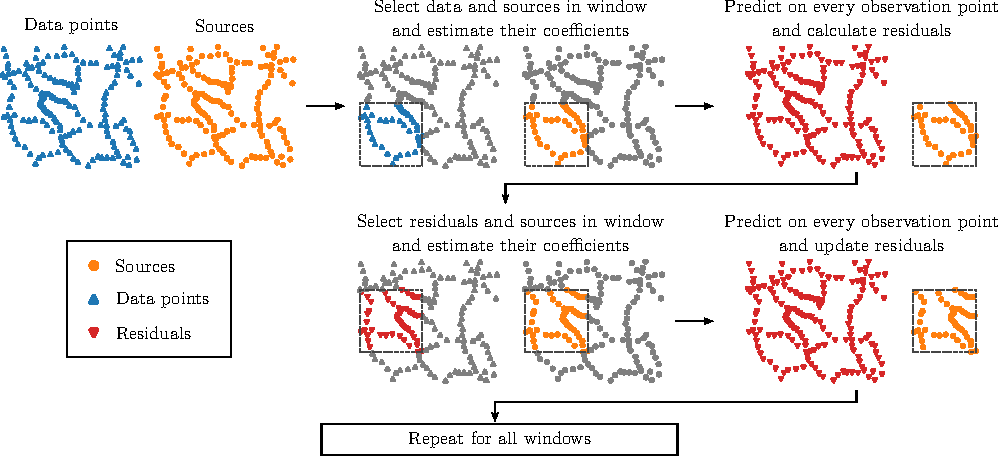
\includegraphics[width=\linewidth]{eql-gradient-boosted/figs/gradient-boosting-schematics.pdf}
    \caption{
        Sketch of the gradient-boosted equivalent source algorithm.
        Data points are represented by blue upwards-facing triangles,
        equivalent sources by orange dots, data residuals by red downwards-facing
        triangles, and the current window by black dashed lines.
        The algorithm starts by selecting the data and sources
        inside the first window and estimating the source coefficients
        using the selected data points.
        Then, the effect of the estimated sources is predicted on all data
        points and used to calculate the residuals.
        Another window is used to select residuals and sources and
        estimate the coefficients using the selected residuals instead of the
        original data.
        Again, the effect of the estimated sources is predicted on all data points
        and the residuals are updated.
        These steps are repeated for every window in a randomized order.
    }
    \label{fig:gradient-boosting-schematics}
\end{figure*}

It is worth noting that two sets of equivalent sources obtained through two
adjacent overlapping windows have some portion of the sources on the same
locations, specifically the ones that fall on the intersection between the two
windows.
We can interpret this as the gradient-boosting algorithm fitting the source
coefficients multiple times: one time for every window that covers each source.
This fact can be exploited in order to save computer memory.
Instead of storing all of the $\mathbf{c}_k$ vectors
(Eq.~\ref{eq:gb-linear-model}), we can initialize a single $\mathbf{c}$ vector
with zeros, where each element represents the coefficient of each one of the
original $M$ sources.
After each iteration of the gradient-boosting algorithm, we add the estimated
coefficients $\hat{\mathbf{c}}_k$ to the corresponding elements of vector
$\mathbf{c}$.
Because the forward modelling function is linear, we can safely compute the
resulting field through Eq.~\ref{eq:eql-forward} instead of
Eq.~\ref{eq:eql-forward-gb}.
This way, the memory needed to store the entire set of estimated coefficients
is limited to a single vector of $M$ elements.

Our gradient boosting algorithm for overlapping windows is similar to the
``bootstrap inversion'' used in \citet{vonfrese1988}, which also iteratively
fits portions of an equivalent source model to the data residuals.
The key differences are that in our method:
(i)~the sources in the overlapping portions of the windows are fitted more than
once, allowing the algorithm to self-correct for poor solutions to any given
window;
(ii)~we use only data points within the window when fitting, what enables the
use of larger datasets.



\subsection{Location of sources}
\label{sec:source_distribution}

The ideal number of sources and their locations, both horizontally and
vertically, has been debated since the inception of the equivalent sources
technique with \citet{dampney1969}.
The choices made regarding these parameters can play an important role on the
accuracy of the predictions and the computational resources needed to estimate
the source coefficients.
An ideal distribution of sources should simultaneously be able to reproduce the
measured data on the survey points, make accurate predictions on non-surveyed
locations, and minimize the required computational resources.

A large number of evenly distributed sources along the survey region are
capable of reproducing the observed data.
Nevertheless, the computational load can be prohibitive and such
underdetermined problems are prone to overfitting the data, leading to poor
predictive power when interpolating and extrapolating.
On the other hand, using few sources will reduce the computational requirements
but the model may be incapable of reproducing the full spectral content of the
measured data.

Particular survey characteristics also play a role in the choice of equivalent
source distribution.
In a ground survey, observations are usually located along irregular paths and
scattered points.
The coverage of the survey region is often uneven, leaving large areas without
any observation.
On the other hand, observations from airborne surveys are located along almost
straight and closely spaced flight lines.
Measurements are usually taken at a high temporal frequency, leading to
observation points along the flight lines that are several times closer to each
other than the flight line spacing.
This creates a bias in the sampling, which can cause aliasing artifacts in
gridded products.

\subsubsection{Horizontal source layouts}

\begin{figure*}[tb!]
    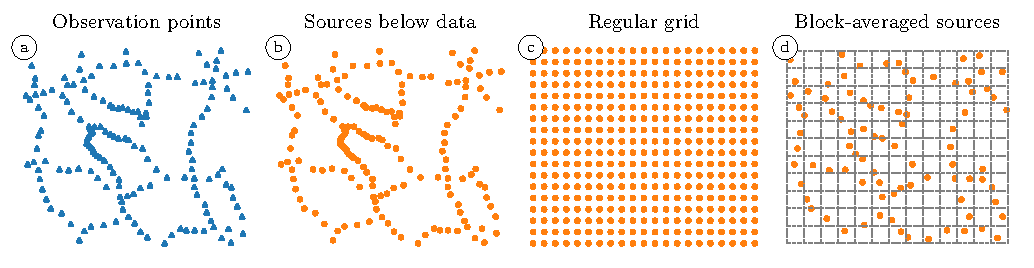
\includegraphics[width=\linewidth]{eql-gradient-boosted/figs/source-layouts-schematics.pdf}
    \caption{
        Sketch of different horizontal layouts for equivalent source models.
        Blue points represent the locations of observations and orange points
        represent the locations of equivalent sources according to different
        layout strategies.
        (a)~Set of \SourceLayoutsSchematicsObservations{} observation points
        that simulate a ground survey.
        (b)~Location of the \SourceLayoutsSchematicsSourceBelowData{} sources
        obtained through the \emph{sources below data} layout.
        (c)~Location of the \SourceLayoutsSchematicsGridSources{} sources
        obtained through the \emph{regular grid} layout.
        (d)~Location of the \SourceLayoutsSchematicsBlockAveragedSources{}
        sources obtained through the \emph{block-averaged sources} layout.
        Grey dashed lines represent the spatial blocks within which the median
        observation location is calculated.
    }
    \label{fig:source_layouts}
\end{figure*}

The most widely used layouts for distributing equivalent sources horizontally
are:

\begin{enumerate}
  \item
    \emph{Sources below data points}: one equivalent source is placed at the
    horizontal location of each data point (Fig.~\ref{fig:source_layouts}b).
    Therefore, the number of sources is equal to the number of observations
    ($M=N$).
  \item
    \emph{Regular grid}: a homogeneous distribution of point sources below the
    survey region (Fig.~\ref{fig:source_layouts}c). A padding region is often
    added to help reduce edge effects. In practice, it often leads to
    underdetermined problems since a large number of sources is required
    ($M>N$).
\end{enumerate}

For ground surveys, the \emph{regular grid} layout needs a sufficiently
small grid spacing to be able to fit the observed data.
This creates an unnecessarily large number of sources in areas where no
observations exist.
In contrast, the \emph{sources below data} layout is more likely to accurately
fit the observed data with many fewer sources, reducing the computational load.
But when applied to airborne surveys, the \emph{sources below data} layout may
place an undesirably large number of sources along the flight paths.
This could lead to aliasing effects on the predicted values, such as the
stripes parallel to flight lines that are often observed when gridding airborne
magnetic data.
The \emph{regular grid} layout can avoid this effect by evenly
distributing sources and using a continuous source layer (e.g.,
right-rectangular prisms or tesseroids).

We propose a new way of distributing equivalent sources horizontally that could
simultaneously reduce the computational load and mitigate some of the drawbacks
of existing layouts.
In the \emph{block-averaged sources} layout,
point sources are placed in the average
position of data points that fall within specified spatial blocks
(Fig.~\ref{fig:source_layouts}d).
This is done by:

\begin{enumerate}
    \item Dividing the survey region into rectangular blocks of equal size.
    \item \label{item:median-position} Computing the median horizontal position
        of the observation points that fall inside each block. Blocks without
        any observation point are omitted.
    \item Assign one point source to each of the median horizontal positions
      calculated in step \ref{item:median-position}.
\end{enumerate}

The number of sources created by this new layout will be less than the number
of observations if the block size is chosen appropriately (i.e., making sure
that blocks are large enough to contain more than a single data point).
The overdetermined problem that arises from this layout has a lower
computational load and is less prone to overfitting the data since the model
complexity is lower.
Moreover, the block averaging process can balance the spacing between sources
along a flight line and between adjacent lines, helping to reduce aliasing
effects in the generated grids.
In Section~\ref{sec:synthetic_distributions}, we demonstrate through tests on
synthetic data that the block-averaged sources layout is able to interpolate
with comparable accuracy to other layouts while using a fraction of the
equivalent sources.


\subsubsection{Depth of sources}

\begin{figure*}[tb!]
    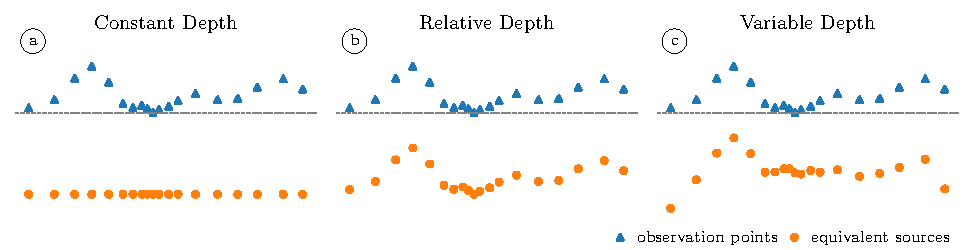
\includegraphics[width=\linewidth]{eql-gradient-boosted/figs/depth_types.pdf}
    \caption{
        Examples of different strategies for assigning depths to equivalent
        sources.
        Here we assign one source for each
        observation point, located at the same horizontal coordinates as the
        data points.
        Source depths are
        (a)~a \emph{constant depth} at a chosen vertical coordinate,
        (b)~a \emph{relative depth} determined by uniformly shifting downward
        the vertical coordinate of data points,
        and
        (c)~a \emph{variable depth} determined by shifting the vertical
        coordinates of the observation points by an amount proportional to the
        average distance to neighbouring sources.
        The distance between data points and their respective sources (a)
        depends on observation height, (b) is constant, and (c) is proportional
        to the horizontal distribution of sources.
        Notice how the closely spaced sources in the middle of the profile (c)
        are shallower than their counterparts in (b).
    }
    \label{fig:depth_types}
\end{figure*}

It is widely known from potential theory that the depth of a point source
influences the wavelength of the observed field at the surface.
This makes the source depth a key parameter affecting the outcome of
interpolation and other operations done with equivalent sources.
Several different strategies for assigning the depths of equivalent sources
have been proposed in the literature.
Here, we will highlight the following (Fig.~\ref{fig:depth_types}):

\begin{enumerate}
  \item
    \emph{Constant depth}:
    The simplest option is to locate all sources at the same depth
    (Fig.~\ref{fig:depth_types}a).
    If the measurements were taken at significantly different altitudes, some
    measurements will be more distant to the sources than others,
    which may create problems for reproducing short wavelengths in high
    altitude points.
 \item
    \emph{Relative depth}:
    The depths of sources are determined by shifting the vertical coordinate of
    data points downward by a fixed amount (Fig.~\ref{fig:depth_types}b).
    The sources will not all be at the same vertical coordinate, but they will
    all be at the same vertical distance from the observation points.
 \item
    \emph{Variable depth}:
    The depths of sources are proportional to the horizontal distance to the
    nearest neighbouring data points or sources (Fig.~\ref{fig:depth_types}c).
    Different variations of this strategy have been proposed before, for
    example \citet{cordell1992}, \citet{guspi2004}, and \citet{Guspi2009}.
    The rationale for this strategy is that if a survey has data points
    clustered in some areas, we may
    want the sources below those areas to be shallower in order to preserve the
    shorter wavelengths that can be measured.
\end{enumerate}

Our approach to the \emph{variable depth} strategy will be:

\begin{equation}
  z = z_{obs} + \Delta z + \alpha h,
  \label{eq:variable_depth}
\end{equation}

\noindent
in which $z$ is the vertical coordinate (positive downwards) of an equivalent
source,
$\Delta z$ is a relative depth shift that is the same for all sources,
$\alpha$ is an dimensionless depth factor,
$h$ is the median horizontal distance to the $k$ nearest neighbouring sources,
and
$z_{obs}$ is a vertical observation coordinate that will depend on the
horizontal layout strategy.
For \emph{sources below data}, it is the vertical coordinate of the data point
corresponding to the given source.
For \emph{regular grid}, it can be interpolated from the vertical coordinates
of all data points.
Finally, for \emph{block-averaged sources} it will be the median vertical
coordinate of the data within the corresponding block.

In Section~\ref{sec:synthetic_distributions}, we test the effectiveness each of
these strategies on synthetic data.

%%%%%%%%%%%%%%%%%%%%%%%%%%%%%%%%%%%%%%%%%%%%%%%%%%%%%%%%%%%%%%%%%%%%%%%%%%%%%%%

\section{Tests on synthetic data}

\begin{figure*}[tb!]
    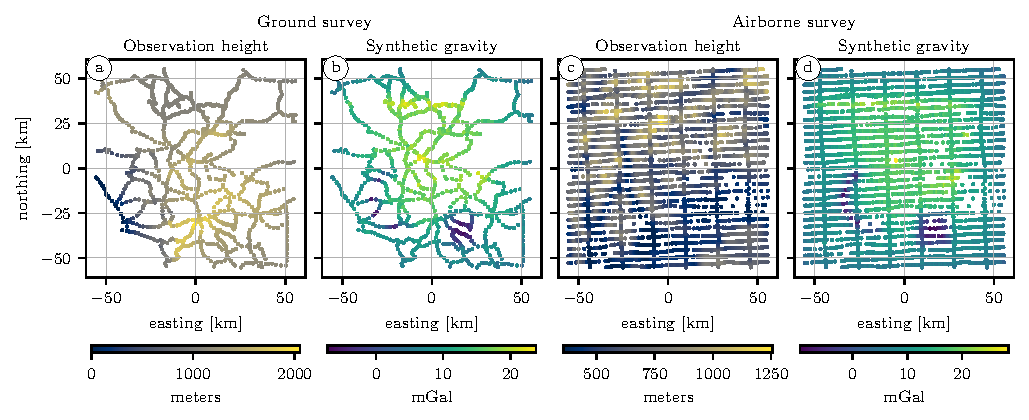
\includegraphics[width=\linewidth]{eql-gradient-boosted/figs/synthetic-survey-layouts.pdf}
    \caption{
        Observation heights and gravity values for the synthetic ground (a-b)
        and airborne (c-d) surveys.
        Heights are given in meters above the zero height plane.
        The synthetic gravity data are contaminated with pseudo-random Gaussian
        noise with zero mean and \SurveyNoise{} standard deviation.
    }
    \label{fig:synthetic-layouts}
\end{figure*}

\begin{figure}[tb!]
    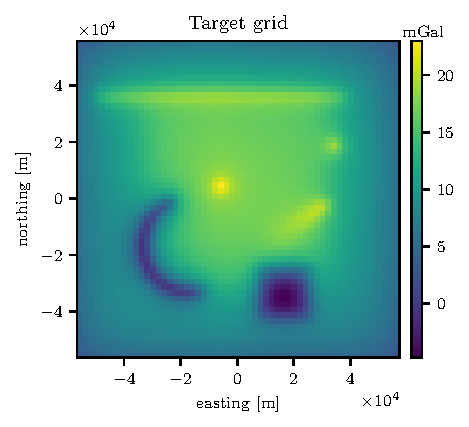
\includegraphics[width=\linewidth]{eql-gradient-boosted/figs/target-grid.pdf}
    \caption{
        Pseudo-color map of the target grid of synthetic gravity data. The grid
        is composed of \TargetEastingSize{}$\times$\TargetNorthingSize{} points
        with a spacing of \TargetSpacing{}. The grid height is \TargetHeight{}
        above the zero height plane.
    }
    \label{fig:synthetic-target}
\end{figure}

We have used synthetic gravity datasets to test the interpolation accuracy of
the difference horizontal and vertical source distribution strategies as well
as the gradient-boosted equivalent sources method.
To generate the data, we created a model of \NPrisms{} right-rectangular
prisms,
distributed in a \ModelEasting{}$\times$\ModelNorthing{} area with depths
varying between \ModelDepth{} and zero.
The density contrast of prisms ranges from \ModelMinDensity{} to
\ModelMaxDensity{}.
The model includes prisms of different shapes, sizes, and depths to create
gravity disturbances with a variety of wavelengths.

We created two synthetic datasets from the model, one simulating a ground
survey and another an airborne acquisition (Fig.~\ref{fig:synthetic-layouts}).
To create the synthetic ground survey, we selected measurement positions from a
portion of a public domain gravity dataset for Southern Africa, available
through the NOAA National Centers for Environmental Information (NCEI).
For the synthetic airborne survey, we used a portion of the Great Britain
Aeromagnetic Survey acquired by Hunting Geology and Geophysics Ltd and Canadian
Aeroservices Ltd between 1955 and 1965 and made publicly available by the
British Geological Survey (BGS).
In both cases, we rescaled the horizontal coordinates of each survey portion to
span an area of \SurveyEasting{}$\times$\SurveyNorthing{}, matching the model
dimensions.
The ground survey contains \GroundSurveyPoints{} observations distributed at
heights between \GroundSurveyMinHeight{} and \GroundSurveyMaxHeight{}
(Fig.~\ref{fig:synthetic-layouts}a).
The airborne survey has \AirborneSurveyPoints{} observations at heights between
\AirborneSurveyMinHeight{} and \AirborneSurveyMaxHeight{}
(Fig.~\ref{fig:synthetic-layouts}c).

The vertical component of the gravitational acceleration generated by the
model was computed  using the method of \citet{nagy2000, nagy2002}
with recent modifications by \citet{fukushima2020},
as implemented in the open-source software Harmonica \citep{harmonica2020}.
We generated a \emph{target grid} of
\TargetEastingSize{}$\times$\TargetNorthingSize{} points with a spacing of
\TargetSpacing{} and located \TargetHeight{} above the zero height plane
(Fig.~\ref{fig:synthetic-target}) to serve as a reference when calculating the
interpolation error.
We then generated synthetic ground (Fig.~\ref{fig:synthetic-layouts}b) and
airborne (Fig.~\ref{fig:synthetic-layouts}d) data to which we added
pseudo-random Gaussian noise with zero mean and \SurveyNoise{} standard
deviation.


\subsection{Source distribution strategies}
\label{sec:synthetic_distributions}

\begin{figure*}[p]
    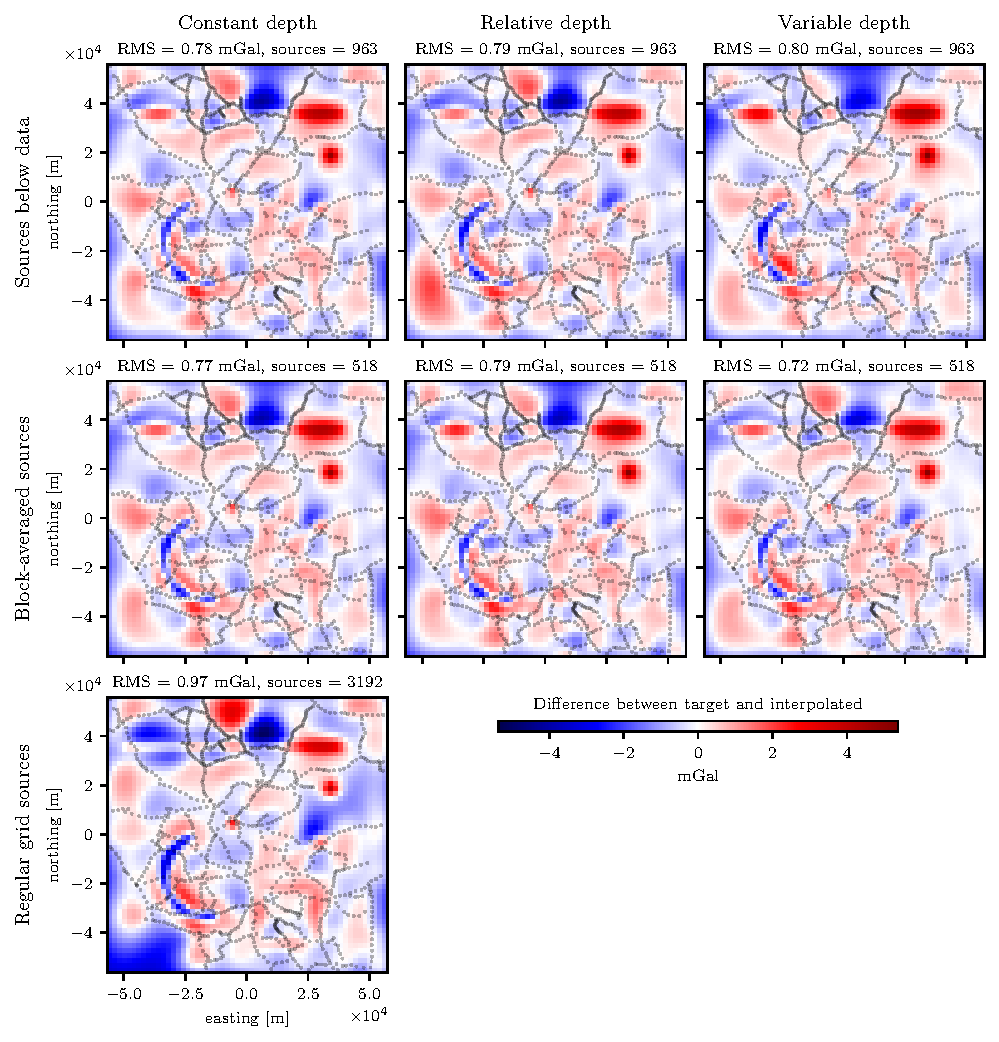
\includegraphics[width=\linewidth]{eql-gradient-boosted/figs/ground_survey_differences.pdf}
    \caption{
        Pseudo-color maps of the differences between the target grid and the
        interpolated synthetic ground survey data produced by each source
        distribution strategy.
        The black dots represent the horizontal location of the synthetic data
        points. The RMS error and total number of equivalent sources is
        reported for each strategy at the top of the respective maps.
    }
    \label{fig:ground-survey-differences}
\end{figure*}

\begin{figure*}[p]
    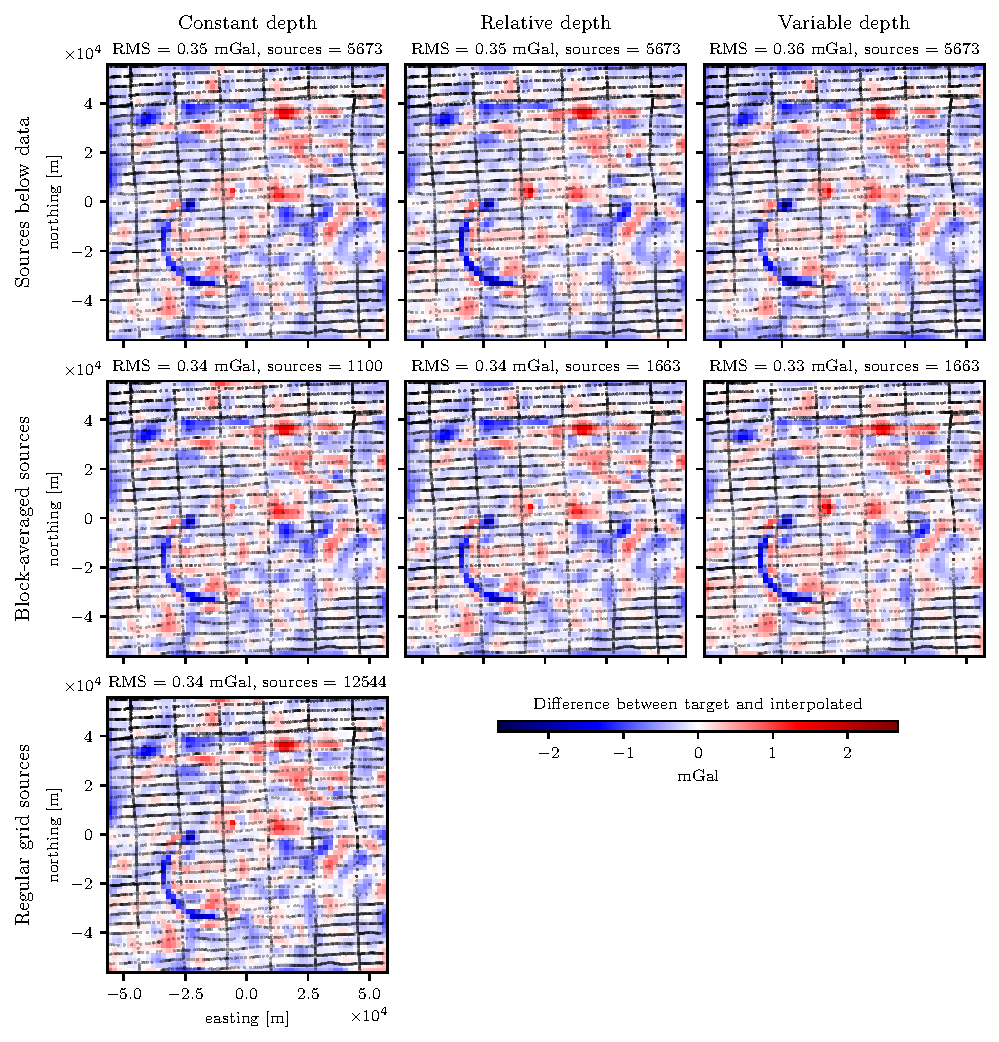
\includegraphics[width=\linewidth]{eql-gradient-boosted/figs/airborne_survey_differences.pdf}
    \caption{
        Pseudo-color maps of the differences between the target grid and the
        interpolated synthetic airborne survey data produced by each source
        distribution strategy.
        The black dots represent the horizontal location of the synthetic data
        points. The RMS error and total number of equivalent sources is
        reported for each strategy at the top of the respective maps.
    }
    \label{fig:airborne-survey-differences}
\end{figure*}

We investigated the effect on interpolation accuracy of different strategies
for distributing the equivalent sources horizontally and vertically.
To do this, we used the damped least-squares solution described in
Section~\ref{sec:eql_inversion} (without gradient boosting) to interpolate the
synthetic datasets (Fig.~\ref{fig:synthetic-layouts}) and compared the results
against the target grid (Fig.~\ref{fig:synthetic-target}).
This process was repeated for each combination of horizontal layout
(\emph{sources below data} and \emph{block-averaged sources}) and depth type
(\emph{constant}, \emph{relative}, and \emph{variable}) and for regular grid
sources with a constant depth, totalling 7 different combinations.

Each source distribution strategy requires certain hyper-parameters to be
chosen in order to build the set of point sources.
For example, using a constant depth needs the definition of the depth and using
block-averaged sources requires the definition of the block size.
The predictive capabilities of the equivalent sources depend on the choice of
these hyper-parameters.
To ensure that our comparisons are fair, we perform an exhaustive search over
combinations of hyper-parameter values (including the damping parameter from
Eq.~\ref{eq:misfit}) to obtain the best prediction that can be achieved by each
source distribution strategy.
Here, the best prediction is defined as the one that minimizes the root
mean-square error (RMS) between interpolated values and the target grid
(Fig.~\ref{fig:synthetic-target}).
The parameter values used in these searches and the one producing the smallest
RMS error are outlined in Tables~\ref{tab:parameters-ground-survey}
and~\ref{tab:parameters-airborne-survey}.

Fig.~\ref{fig:ground-survey-differences}
and~\ref{fig:airborne-survey-differences} show the differences between the
target grid and the best prediction achieved by each source distribution
strategy for the ground and airborne synthetic surveys, respectively.
For the synthetic ground survey, the horizontal layouts produced similar RMS
values of approximately 0.8\mGal{} regardless of the depth type, with the
exception of the regular grid layout which produced a larger RMS of
\BestGroundGridSourcesConstantDepthRms{}\mGal{}.
The differences between the target grid and the interpolated values are larger
in regions of poor data coverage.
Edge effects are present for all strategies but are noticeably smaller for the
combination of block-averaged sources with a variable depth based on the
nearest neighbour distance.
For the synthetic airborne survey, all strategies (including the regular grid)
produced similar RMS errors of approximately 0.3\mGal{}.
The maps of the differences between the target grid and interpolation results
are visually indistinguishable from each other.

%%%%%%%%%%%%%%%%%%%%%%%%%%%%%%%%%%%%%%%%%%%%%%%%%%%%%%%%%%%%%%%%%%%%%%%%%%%%%%%


\subsection{Window size and overlap in gradient boosting}
\label{sec:window_size_and_overlap}

We assessed the trade-offs in interpolation accuracy and computation time of
the gradient-boosted equivalent sources algorithm as a function of the two key
controlling factors: the window size and the amount of overlap between adjacent
windows.
The comparisons were performed against a regular least-squares solution
(Eq.~\ref{eq:least_squares_solution}) using the synthetic airborne data
(Fig.~\ref{fig:synthetic-layouts}c-d).
To avoid biasing the results, we used the same locations of equivalent sources
for both the regular and gradient-boosted interpolations, namely
block-averaged sources with a block size of
\BestAirborneBlockAveragedSourcesRelativeDepthSpacing\m{} and a
relative depth of
\BestAirborneBlockAveragedSourcesRelativeDepthDepth\m{}.

\subsubsection{Window size}
\label{sec:window_size}

The size of the windows controls the size of the Jacobian matrices
$\tilde{\mathbf{A}}_k$ by limiting the number of data points and equivalent
sources used in each step of the gradient-boosting algorithm
(Alg.~\ref{alg:gradient_boosting_window}).
Thus, using smaller windows will reduce the total amount of computer memory
required to estimate the source coefficients.
Nevertheless, smaller windows may produce less accurate interpolations by
failing to achieve the global minimum of the goal function in
Eq.~\ref{eq:misfit}.
The window size might also impact the computation time in non-intuitive ways
since smaller windows generate smaller least-squares problems but also require
more gradient-boosting iterations.

We calculated the interpolation RMS error (between the interpolated grid and
the target grid in Fig.~\ref{fig:synthetic-target}) and computation time for a
fixed window overlap of 50\% and several window sizes.
To avoid any biases introduced by the shuffling of windows, the calculations
were repeated using different seeds for the pseudo-random number generator used
in the shuffling.
Fig.~\ref{fig:gradient-boosted-comparison}a shows the RMS error and
Fig.~\ref{fig:gradient-boosted-comparison}c shows the computation time
required for estimating the source coefficients, both as functions of
the window size.

\begin{figure*}[tb!]
    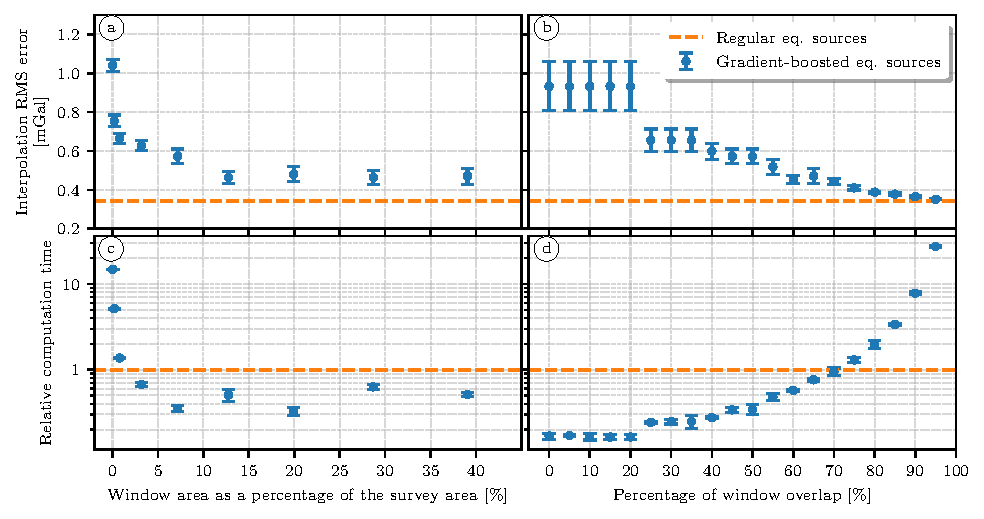
\includegraphics[width=\linewidth]{eql-gradient-boosted/figs/gradient-boosted-comparisons.pdf}
    \caption{
        Interpolation RMS error (a-b) and relative computation time (c-d) for
        regular least-squares equivalent sources (orange dashed lines) and
        gradient-boosted equivalent sources (blue dots and error bars).
        Window overlap is given as a percentage of the window size (an overlap
        of 50\% means that two adjacent windows share an area half of the size
        of the entire window).
        For gradient-boosting, the RMS errors and computation times are the
        means (error bars are 1 standard deviation) of results using different
        seeds for the pseudo-random number generator.
        Computation time is the ratio between the time required to estimate the
        source coefficients for the gradient-boosted and the regular equivalent
        sources.
}
    \label{fig:gradient-boosted-comparison}
\end{figure*}

These results show that the interpolation error for gradient-boosting is
generally larger than the error for regular equivalent sources.
The error decreases asymptotically to within $\sim 40\%$ of the regular
equivalent sources for windows with an area greater than $\sim 10\%$ of the
survey area.
The computation time similarly decreases with window size, with the
gradient-boosting being generally faster than the regular equivalent sources
for windows with an area greater than $\sim 5\%$ of the survey area.
As the window size increases, both RMS error and computation time appear to
stabilize to nearly constant levels.

\subsubsection{Window overlap}

The amount of overlap between adjacent windows plays an important role in the
performance of the gradient-boosted equivalent sources.
It controls the number of iterations and how many times a particular source is
used in the least-squares fitting process.
The experiments in the previous section showed that 50\% overlap was
sufficient to achieve acceptable interpolation accuracy.
However, we studied separately the impacts of the amount of window overlap on
both accuracy and computation time.

We performed a similar experiment to the one in section~\ref{sec:window_size}
but this time kept the window size fixed to \BoostOverlappingWindowSize{} and
varied the amount of overlap from 0\% to 95\% with a step size of 5\%.
All other experimental procedures remained unchanged.
Fig.~\ref{fig:gradient-boosted-comparison}b shows the RMS error and
Fig.~\ref{fig:gradient-boosted-comparison}d shows the computation time
required for estimating the source coefficients, both as functions of
the window overlap.

Our results show that the interpolation RMS error decreases with the amount of
overlap, reaching the same accuracy as the regular equivalent sources at
approximately 90\% overlap.
On the other hand, the computation time increases with the amount of overlap,
becoming larger than that of the regular equivalent sources for overlaps
greater than 70\%.
This is expected since increasing the overlap adds iterations to the gradient
boosting algorithm without decreasing the individual least-squares problem
sizes to compensate.


\subsection{
    Interpolation with gradient boosting
}
\label{sec:gb_interpolation}

Finally, we applied the gradient-boosted equivalent sources to interpolate the
synthetic airborne survey (Fig.~\ref{fig:synthetic-layouts}).
As previously, we used the block-averaged sources layout with a block size of
\EqlBoostAirborneSpacing{}.
Based on the results from section \ref{sec:window_size_and_overlap}, we adopted
a window overlap of 50\% and a window size of \EqlBoostAirborneWindowSize{}.

We estimated the relative depth of the sources and the damping parameter by
comparing the predictions against the values of the target grid.
The search explored \emph{depth} values between \EqlBoostAirborneMinDepth{} and
\EqlBoostAirborneMaxDepth{} and \emph{damping} values between
\EqlBoostAirborneMinDamping{} and \EqlBoostAirborneMaxDamping{} by steps of one
order of magnitude.
The most accurate predictions achieved a RMS error of
\EqlBoostAirborneRmsScore{} with a depth of \EqlBoostAirborneDepth{} and
a damping of \EqlBoostAirborneDamping{}.
It is worth noting that the RMS error achieved by the gradient-boosted
equivalent sources is comparable to the ones obtained by the regular equivalent
sources in Section \ref{sec:synthetic_distributions}.
To highlight the importance of randomizing the order of windows in the
gradient-boosting iterations, we preformed the interpolation once more using
the same values of \emph{damping} and \emph{depth} but this time iterating over
windows in sequential order (South to North, West to East).

\begin{figure}[tb!]
    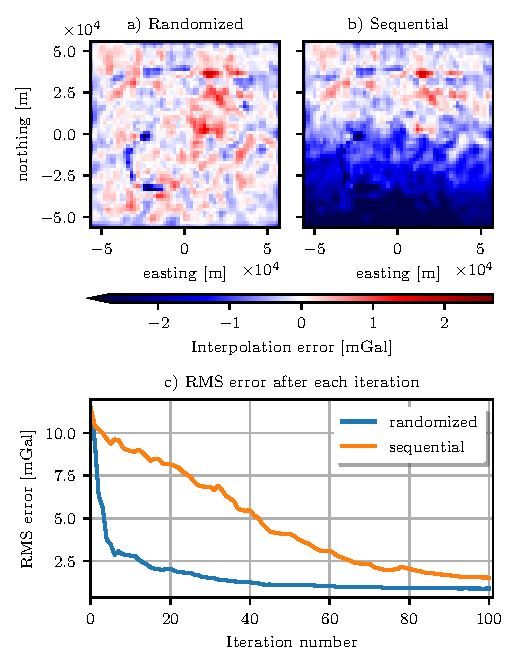
\includegraphics[width=\linewidth]{eql-gradient-boosted/figs/eql-boost-airborne.pdf}
    \caption{
        Interpolation error for gradient-boosted equivalent sources using
        randomized (a) and sequential (b) window order.
        (a and b)~Pseudo-color maps of the differences between the target grid
        and the interpolated synthetic airborne survey data.
        The color scale has been cropped to the same range as
        Fig.~\ref{fig:airborne-survey-differences}.
        (c)~Root-mean squared error after each iteration of the
        gradient-boosting algorithm.
}
\label{fig:eql-boost-airborne}
\end{figure}

Figs.~\ref{fig:eql-boost-airborne}a-b show the differences between the target
grid and the interpolation results for windows in randomized and sequential
order, respectively.
The differences for randomized windows resemble those for regular least-squares
equivalent sources seen in Figs.~\ref{fig:ground-survey-differences} and
\ref{fig:airborne-survey-differences}.
On the other hand, the differences for sequential windows show a clear
trend of large negative differences in the South decreasing towards the North.
This trend is correlated with the order in which windows are executed, with
differences decreasing in absolute value towards the end of the algorithm.
Fig.~\ref{fig:eql-boost-airborne}c shows the RMS error of the fitting process
after each iteration for both window orders, clearly indicating that
a randomized window order leads to faster convergence of the algorithm.


%%%%%%%%%%%%%%%%%%%%%%%%%%%%%%%%%%%%%%%%%%%%%%%%%%%%%%%%%%%%%%%%%%%%%%%%%%%%%%%

\section{Gridding gravity data from Australia}

\begin{figure*}[p]
    \includegraphics[width=\linewidth]{eql-gradient-boosted/figs/australia.png}
    \caption{
      Pseudo-color maps of observed (a and c) and
      interpolated (b and d) gravity disturbance of Australia.
      The observed values in a and c are plotted as colored circles.
      The red rectangle marks the boundaries of the highlight maps in c
      and d.
      Observations are part of a compilation by \citet{wynne2018} of
      over 1.7 million ground gravity measurements.
      Interpolated values were obtained through gradient-boosted equivalent
      sources and calculated on a regular grid at \AustraliaEqlGridHeight{}
      over the WGS84 ellipsoid.
    }
    \label{fig:australia}
\end{figure*}

This section will demonstrate how gradient-boosted equivalent sources can be
used to interpolate large datasets onto regular grids at uniform height.
For this purpose, we selected an open-access compilation of ground gravity
surveys over Australia made by \citet{wynne2018} and filtered and referenced to
the WGS84 ellipsoid by \citet{australia_compilation}.
It contains over 1.7 million data points and covers most of the Australian
territory at variable point spacings.
Our goal is to create a 1~arc-minute resolution grid of gravity disturbances at
a constant geometric height of \AustraliaEqlGridHeight{} (the largest height of
observations).

We computed the gravity disturbance by removing the normal gravity of
the WGS84 ellipsoid from the observed gravity data (Fig.~\ref{fig:australia}).
Here, normal gravity was computed at each observation point through the
closed-form formula of \citet{ligotze2001} using the Boule software
\citep{boule2020}.
Finally, we converted the observations to planar Cartesian coordinates by
applying a Mercator projection.

We start the interpolation process by defining a set of block-averaged sources
using a block size of 1.8\km{}, resulting in a total of
\AustraliaEqlNSources{}~point sources.
The block size was chosen to match the desired resolution of the final grid
(1~arc-minute is approximately 1.8\km{} at the equator).
Based on the results obtained in Section~\ref{sec:synthetic_distributions}, we
have chosen to use the \emph{relative depth} strategy.
The window overlap was once again fixed at 50\%.
To determine the size of the windows, we calculated the amount of computer memory
needed to store the largest Jacobian matrix for different values of window size
(Fig.~\ref{fig:australia-memory-cv-error}a).
We have chosen a size of \AustraliaEqlWindowSize{} in order to limit the
amount of memory needed to under 16~Gigabytes.

\begin{figure}[tbh!]
    \makeatletter%
    \if@twocolumn%
        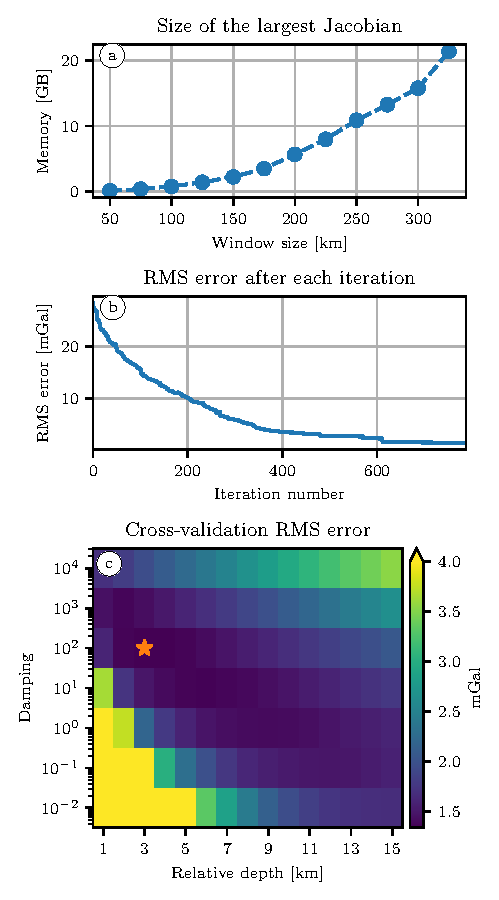
\includegraphics[width=\linewidth]{eql-gradient-boosted/figs/australia-memory-cv-error.pdf}
    \else% \@twocolumnfalse
        \centering
        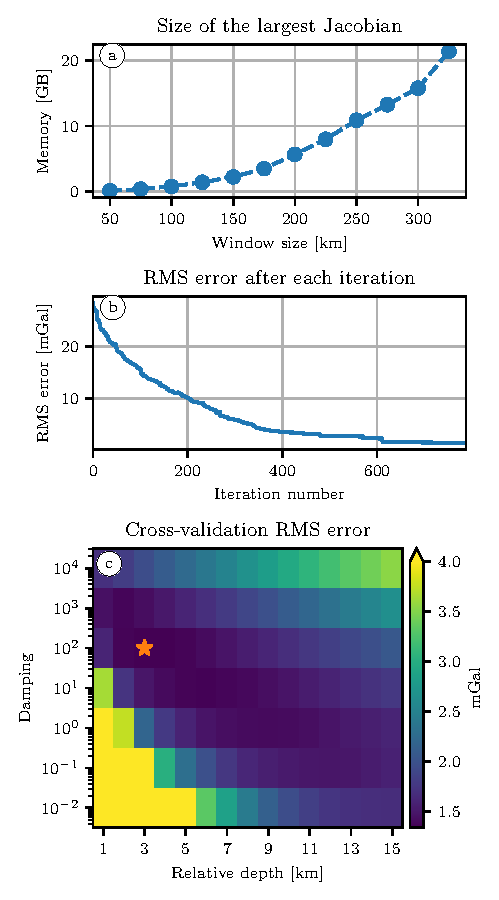
\includegraphics[width=0.6\linewidth]{eql-gradient-boosted/figs/australia-memory-cv-error.pdf}
    \fi
    \makeatother
    \caption{
        (a) Amount of computer memory needed to store the largest Jacobian
        matrix for different window sizes. Our implementation uses double
        precision floating point numbers (64 bits) for the Jacobian.
        (b) Root-mean square error against the observed data after each
        iteration of the gradient-boosting algorithm.
        (c) K-Fold cross-validation root-mean square errors obtained for each
        pair of damping and depth parameters. The orange star highlights the
        minimum.
    }
    \label{fig:australia-memory-cv-error}
\end{figure}

We determined the depth of the sources and the damping parameter by applying
K-Fold cross-validation through the scikit-learn library \citep{sklearn2011}.
The method randomly divides the original data into $k$ sets (folds), fits the
model using only data from $k - 1$ folds, and validates the model by comparing
its predictions against the one remaining fold.
This process is carried out once for each one of the $k$ folds, leading to
an estimated mean cross-validation RMS error for the model.
To speed up the computation, we only performed the cross-validation on a subset
of the data corresponding to an area of
\AustraliaSmallAreaEastingSize{}$\times$\AustraliaSmallAreaNorthingSize{}
containing \AustraliaSmallAreaNPoints{} points.
We ran the cross-validation repeatedly for combinations of \emph{depth},
ranging from \AustraliaDepthMin{} to \AustraliaDepthMax{},
and \emph{damping}, from \AustraliaDampingMin{} to \AustraliaDampingMax{} in
steps of one order of magnitude.
Figure \ref{fig:australia-memory-cv-error}c shows the resulting
cross-validation RMS errors and highlights the minimum value of
\AustraliaEqlRmsScore{}, which corresponds to a relative depth of
\AustraliaEqlDepth{} and a damping equal to \AustraliaEqlDamping{}.

Finally, we proceeded to estimate the source coefficients using the entire
dataset and the parameters previously determined.
The estimated source coefficients were then used to predict the values of the
gravity disturbance on a regular grid of
\AustraliaEqlGridNLongitude{}$\times$\AustraliaEqlGridNLatitude{} points at
\AustraliaEqlGridHeight{} above the ellipsoid.
On a modest workstation with 16 cores and 16~Gigabytes of RAM,
estimating the \AustraliaEqlNSources{} coefficients with gradient-boosting took
$\sim 1.3$~hours and the prediction step took $\sim 18$~minutes.

Fig.~\ref{fig:australia} shows the original data distribution and the
interpolated grid.
Grid points that are further than 50\km{} from the nearest data point are
masked to avoid unrealistic extrapolations.
Fig.~\ref{fig:australia-memory-cv-error}b shows the RMS error against the
observed data after each iteration of the algorithm.
Fig.~\ref{fig:australia-residuals} shows the difference between the observed
and predicted gravity disturbances.
The inset figure shows a histogram of these residuals, which are approximately
normally distributed around zero.

\begin{figure}[tb!]
    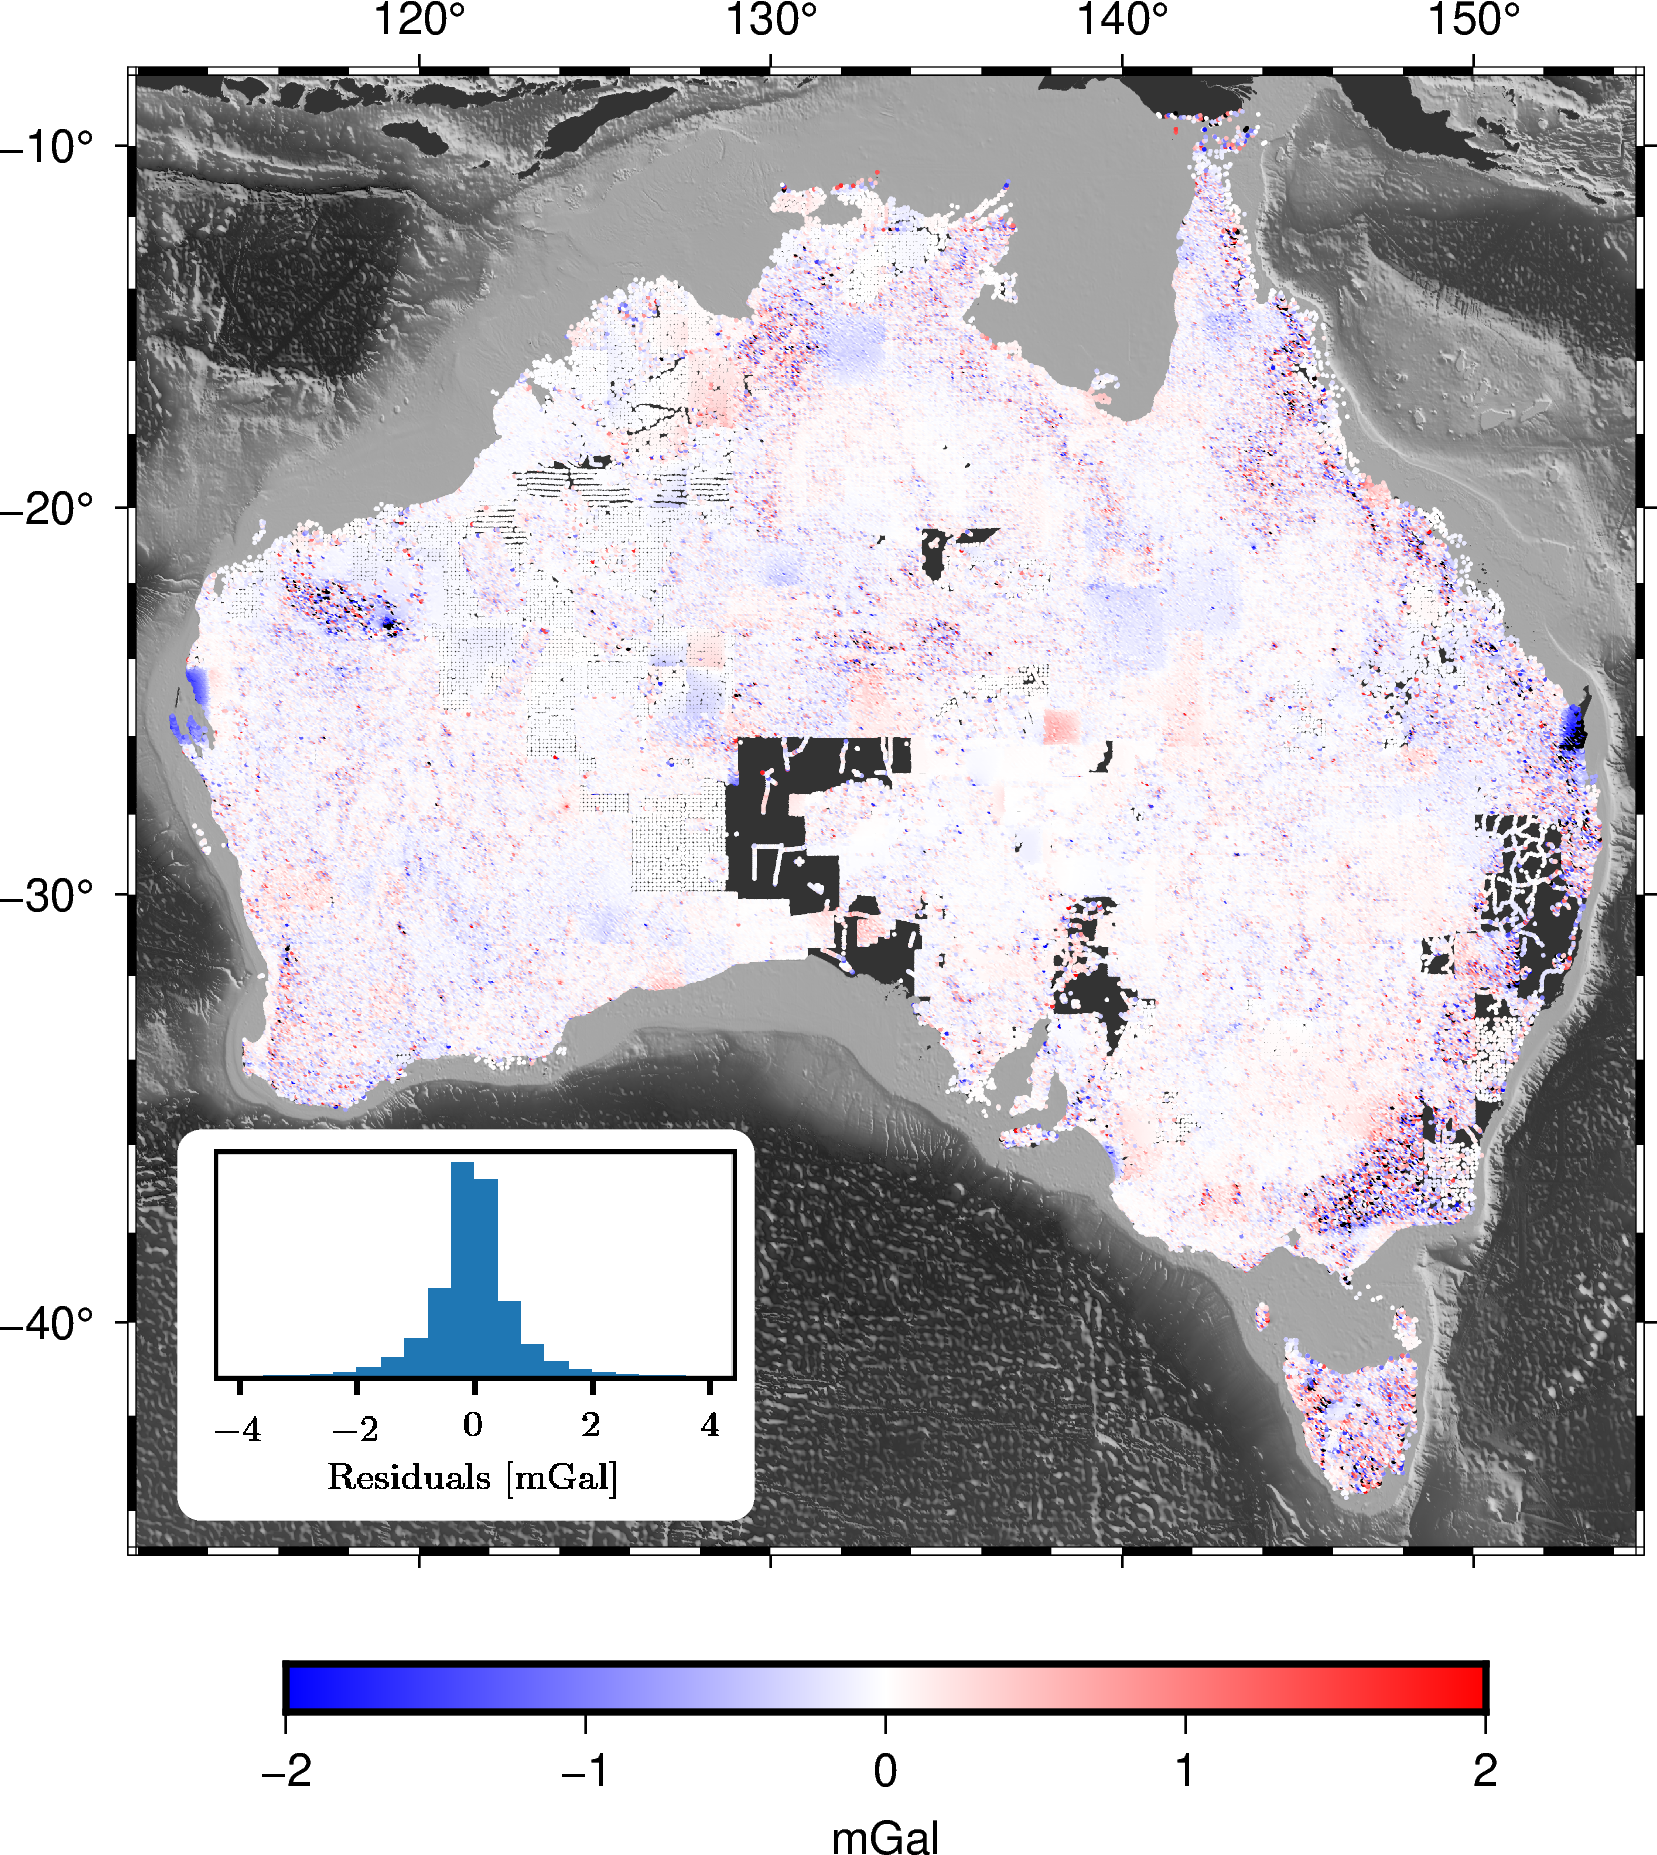
\includegraphics[width=\linewidth]{eql-gradient-boosted/figs/australia-residuals.png}
    \caption{
        Residuals. Differences between the gravity disturbance data from
        Australia and the predicted values by the estimated equivalent sources
        on the same observation points. The color map has been truncated to
        improve the visualization around the largest portion of residual
        values. The inset plot shows a histogram of the residuals.
    }
    \label{fig:australia-residuals}
\end{figure}


%%%%%%%%%%%%%%%%%%%%%%%%%%%%%%%%%%%%%%%%%%%%%%%%%%%%%%%%%%%%%%%%%%%%%%%%%%%%%%%

\section{Discussion}

\subsection{Location of sources}

The results of our tests on synthetic data
(Figs.~\ref{fig:ground-survey-differences}
and~\ref{fig:airborne-survey-differences}) show that there are no significant
differences in interpolation accuracy between source distribution strategies,
both in terms of the interpolation RMS errors and from visual inspection of the
difference maps.
Therefore, we conclude that all source distribution strategies are able to
produce comparable interpolations.
Nevertheless, the \emph{block-averaged sources} strategy makes use of fewer
sources when compared with other strategies, which reduces the computational
load of estimating the sources coefficients and forward modelling.
To ensure that the interpolation is able to reproduce the high frequencies in
the data, the block size used in the averaging should be chosen to match the
desired grid resolution.

The choice of source depth strategy does not appear to significantly impact the
interpolation RMS error.
In the particular case of a sparse ground survey with block-averaged sources,
the use of a variable depth visibly reduced edge effects and artifacts in areas
of poor data coverage.
At a first glance, the choice of a depth strategy would not seem to impact
the computation time.
However, when searching for the set of hyper-parameters that produce the most
accurate interpolation (e.g., through cross-validation), one must solve the
inverse problem once for every possible combination of parameters.
A depth strategy like the \emph{variable depth} requires a higher number of
hyper-parameters (depth shift $\Delta z$, depth factor $\alpha$, and the number
of nearest neighbours $k$ from Eq.~\ref{eq:variable_depth}) than other
strategies which only require a single parameter.
Having more parameters means increasing the dimensions of the parameter space
and thus increasing the number of possible combinations.
Thus, we recommend using a \emph{constant depth} or a \emph{relative depth}
when processing large datasets in order to minimize computation time.

\subsection{Gradient boosting}

From Fig.~\ref{fig:gradient-boosted-comparison}a
and~\ref{fig:gradient-boosted-comparison}c, we can see that the
gradient-boosted equivalent sources produce slightly less accurate
interpolation results but are able to achieve smaller computation times than
regular equivalent sources.
The reduction of the accuracy might be due to the gradient boosting algorithm
failing to converge to the global minimum of the goal function.
As the windows increase in size, interpolation error decreases because more data
points are included into the least-squares fitting of the source coefficients.
At the same time, the fitting process becomes faster because of a reduction in
the number of iterations.
Our results indicate that it is desirable to maximize the window size,
which can be done up to the point that the Jacobian matrices still fit within
the available computer memory.

The results shown in Figs.~\ref{fig:gradient-boosted-comparison}b
and~\ref{fig:gradient-boosted-comparison}d indicate that using
window overlap values between 40\% and 70\% strike a balance between
accuracy and computation time.
This corroborates our initial choice of 50\% overlap, which is good enough for
producing accurate predictions in reasonable times.

Finally, the results in Fig.~\ref{fig:eql-boost-airborne} highlight the
importance of randomizing the order in which the overlapping windows are
iterated.
Running the gradient boosting algorithm sequentially produces less accurate
predictions and decreases the convergence rate of the method.

\subsection{Australia gravity data}

The application of the gradient-boosted equivalent sources to the Australian
gravity dataset demonstrates that the method is able to interpolate and
upward-continue large datasets in a reasonable amount of time using only modest
computational resources.
The resulting grid (Fig.~\ref{fig:australia}) preserves the high resolution of
the original data while avoiding aliasing artifacts due to the block averaging
of the source locations.
Some parts of the grid are smoother and have lower amplitudes than the original
data (e.g., some southwestern parts), which is expected from the upward
continuation that was performed to have the grid at a constant height.
From the cross-validation analysis on a subset of the data, we estimate that
the interpolation error is approximately \AustraliaEqlRmsScore{}.

The largest residuals in Fig.~\ref{fig:australia-residuals} are located in
regions with high-amplitude short-wavelength features in the observed data.
This is expected since the method involves some degree of smoothing because of
the use of damping and the source depths.
There are also low-amplitude long-wavelength residual signals that seem to
coincide with some of the windows of the gradient-boosting method.
A possible cause of these features is inability of the equivalent-sources
within a window to adequately fit the long-wavelength components of the data.
We note, however, that all of these long-wavelength residuals are smaller than
1\mGal{} in amplitude and do not represent a significant source of errors.

The elongated valley around the minimum of the cross-validation RMS errors
(Fig.~\ref{fig:australia-memory-cv-error}c) shows that there is ambiguity in
the choice of damping and source depths.
One could choose a large damping with a small depth or a small damping with a
large depth to achieve roughly the same interpolation result.
This is expected since both parameters control the smoothness of the
interpolation.

%%%%%%%%%%%%%%%%%%%%%%%%%%%%%%%%%%%%%%%%%%%%%%%%%%%%%%%%%%%%%%%%%%%%%%%%%%%%%%%

\section{Conclusions}

The equivalent source technique has been proven to be well suited for
interpolating gravity disturbances and magnetic anomalies.
The two main reasons that make it to stand out from other 2D interpolation
methods is the fact that the equivalent sources take into account the height of
the observations and that the interpolated values will always be harmonic
functions.
The main challenge of using equivalent sources in practice is the high
computational load of estimating the coefficients of the equivalent sources,
specially the computer memory needed to store the Jacobian matrix.

We present two strategies that could be simultaneously applied to interpolate
datasets with millions of points on modest hardware:
block-averaging source locations, which reduces the number of equivalent
sources needed for the interpolation,
and the gradient-boosted equivalent source algorithm, which breaks down the
inverse problem into smaller sets of equivalent sources defined by overlapping
windows.
Both methods were tested against synthetic datasets in order to compare their
accuracy and how they perform in terms of computational efficiency.

Our results show that the block-averaged sources reduce the computational
load needed to estimate source coefficients in comparison to two traditional
strategies (placing sources below data points or on regular grids).
We also show that this reduction of the number of sources does not affect
the accuracy of the predictions.
The use of block-averaged sources may also prevent aliasing of the interpolated
values, specially when the observations are unevenly sampled (e.g., airborne
and shipborne surveys).
Special attention must be payed when choosing the size of the blocks for
averaging.
As a thumb rule, we recommend choosing a size approximately equal to
the resolution of the regular grid where the values will be interpolated.

Tests that compared strategies for the vertical location of the
sources showed that any one of the three strategies tested
(\emph{constant depth}, \emph{relative depth} and \emph{variable depth})
produces comparable accuracy of interpolation.
Nevertheless, we are more prone to recommending either the \emph{constant
depth} or the \emph{relative depth} for most applications because they involve
less hyper-parameters that would need to be configured before the actual
interpolation.

Gradient-boosted equivalent sources were shown to heavily reduce the computer
memory needed to estimate source coefficients, making it possible to
interpolate large datasets with millions of points that would otherwise produce
Jacobian matrices larger than the available memory.
The interpolations obtained though this new method achieve close to the same
accuracy than the regular equivalent sources, while reducing the computation
time by approximately a factor of three.
We also show that an overlap of 50\% between adjacent windows achieves a good
compromise between accuracy and computation time.
The size of the overlapping windows should be chosen as the maximum value
possible that creates Jacobian matrices that still fit into computer memory.
Moreover, randomizing the order in which the windows are iterated increases the
convergence rate of the algorithm and is essential to producing accurate
predictions.

The gradient-boosting method can be used in conjunction with any horizontal
source layout, depth strategy, or source type (e.g., point sources, prisms,
tesseroids) because it does not rely on assumptions about the sources.
Future research should investigate the application of gradient boosting to
other equivalent source methods.

%%%%%%%%%%%%%%%%%%%%%%%%%%%%%%%%%%%%%%%%%%%%%%%%%%%%%%%%%%%%%%%%%%%%%%%%%%%%%%%

\section*{Data and code availability}

The Python source code used to produce all results and figures presented here
is available at
\url{https://doi.org/10.6084/m9.figshare.13604360} and
\url{https://github.com/compgeolab/eql-gradient-boosted}
under the BSD 3-clause open-source license.

The gradient-boosted equivalent sources implementation is based on the
equivalent source code in the Harmonica library \citep{harmonica2020}.
Other software used in this study includes:
Pooch \citep{pooch2020} for downloading and caching datasets,
Verde \citep{verde2018} for block reductions and coordinate manipulations,
Boule \citep{boule2020} for normal gravity calculations,
xarray \citep{xarray2017} and Numpy \citep{numpy} for handling
multidimensional arrays and numerical computations,
Numba \citep{numba2015} for just-in-time compilation and parallelization,
scikit-learn \citep{sklearn2011} for cross-validation,
Matplotlib \citep{Hunter2007} and PyGMT \citep{pygmt2020} for generating
the figures and maps,
and the Jupyter notebook programming environment \citep{jupyter2016}.
Harmonica, Boule, Pooch, and Verde are part of the Fatiando a Terra project
\citep{Uieda2013}.

All datasets used are open-access and publicly available.
The synthetic surveys were generated using
a public domain gravity dataset for Southern Africa distributed by the
NOAA NCEI (\url{https://www.ngdc.noaa.gov/mgg/gravity/gravity.html})
and the Great Britain Aeromagnetic
Survey distributed by the
British Geological Survey (BGS) under an Open Government License
(\url{https://www.bgs.ac.uk/products/geophysics/aeromagneticRegional.html}).
The shaded relief in Fig.~\ref{fig:australia} is the SRTM15+ dataset by
\citet{tozer2019}.
The Australian ground gravity
data is based on a compilation distributed by Geoscience Australia under a
Creative Commons Attribution 4.0 International Licence \citep{wynne2018}  which
was filtered and referenced to the WGS84 ellipsoid by
\citet{australia_compilation} and is distributed under the same license
(\url{https://doi.org/10.6084/m9.figshare.13643837}).


%%%%%%%%%%%%%%%%%%%%%%%%%%%%%%%%%%%%%%%%%%%%%%%%%%%%%%%%%%%%%%%%%%%%%%%%%%%%%%%

\section*{Acknowledgements}

We are indebted to the developers and maintainers of the open-source software
without which this work would not have been possible.
We would also like to thank Editor Frederik Simons, Assistant Editor Fern
Storey, and two anonymous reviewers for their constructive comments.
S.R. Soler is supported by a scholarship from CONICET, Argentina.
This work contains British Geological Survey materials ©~UKRI.
S.R. Soler and L. Uieda jointly developed the initial idea, analysed the
results, and wrote the paper. S.R. Soler produced all results and developed the
software implementation with the assistance of L. Uieda.

\endgroup

%==============================================================================
\chapter{Dual-layer magnetic equivalent sources}

%==============================================================================
\chapter{Magnetic microscopy inversion}

%==============================================================================
\chapter{Iterative magnetic microscopy inversion}

%==============================================================================
\chapter{Euler inversion}

\begingroup
% Used to set information about the paper that is used in multiple files
%%%%%%%%%%%%%%%%%%%%%%%%%%%%%%%%%%%%%%%%%%%%%%%%%%%%%%%%%%%%%%%%%%%%%%%%%%%%%%%

% Set variables with the title, authors, etc.
\newcommand{\Title}{Euler inversion: Locating sources of potential-field data through inversion of Euler's homogeneity equation}
\newcommand{\TitleShort}{Euler inversion}

\newcommand{\Year}{2025}
\newcommand{\PreprintOn}{2024/12/19}
\newcommand{\SubmittedOn}{2024/12/20}
\newcommand{\RevisionAOn}{2025/02/28}
\newcommand{\PublishedOn}{2025/03/26}

\newcommand{\Authors}{%
  Leonardo Uieda\textsuperscript{1},
  Gelson Ferreira Souza-Junior\textsuperscript{1},
  India Uppal\textsuperscript{2},
  Vanderlei Coelho Oliveira Jr.\textsuperscript{3}
}
\newcommand{\Affiliations}{%
  \textsuperscript{1} Universidade de São Paulo, Brazil;
  \textsuperscript{2} University of Liverpool, UK;
  \textsuperscript{3} Observatório Nacional, Brazil;
}

\newcommand{\Journal}{Geophysical Journal International}
\newcommand{\JournalDOI}{10.1093/gji/ggaf114}
\newcommand{\PreprintDOI}{10.31223/X5T41M}
\newcommand{\ArchiveDOI}{10.6084/m9.figshare.26384140}
\newcommand{\GitHubRepository}{compgeolab/euler-inversion}
\newcommand{\SWHeritageID}{swh:1:snp:b0d1f8fdbf57f87e0ce56d5dda0f360c4a314d9d}
\newcommand{\SWHeritageURL}{https://archive.softwareheritage.org/\SWHeritageID;origin=https://github.com/\GitHubRepository}

\newcommand{\RioNSources}{\num{300}}
\newcommand{\RioWindowSize}{\qty{12000}{\m}}
\newcommand{\RioWindowStep}{\qty{2400}{\m}}
\newcommand{\RioWeightsF}{\num{1}}
\newcommand{\RioWeightsE}{\num{0.1}}
\newcommand{\RioWeightsN}{\num{0.1}}
\newcommand{\RioWeightsU}{\num{0.05}}
\newcommand{\RioPercentile}{\num{99.5}}
\newcommand{\RioSIMin}{1}
\newcommand{\RioSIMax}{3}\newcommand{\RioNData}{\num{50882}}
\newcommand{\RioDerivSpacing}{\qty{1}{\m}}
\newcommand{\RioEQSDepth}{\qty{1000}{\m}}
\newcommand{\RioEQSDamping}{\num{10}}
\newcommand{\RioEQSBlock}{\qty{100}{\m}}
\newcommand{\RioEQSWindow}{\qty{22313}{\m}}\newcommand{\SynInterfDykesDistMax}{\qty{9000}{\m}}
\newcommand{\SynInterfDykesDistMin}{\qty{1000}{\m}}
\newcommand{\SynInterfDykesTrueEast}{\qty{7000}{\m}}
\newcommand{\SynInterfDykesTrueNorth}{\qty{4500}{\m}}
\newcommand{\SynInterfDykesTrueUp}{\qty{0}{\m}}
\newcommand{\SynInterfDykesTrueBase}{\qty{100}{\nano\tesla}}
\newcommand{\SynInterfDykesInterfEastMax}{\qty{6000}{\m}}
\newcommand{\SynInterfDykesInterfEastMin}{\qty{-2000}{\m}}
\newcommand{\SynInterfDykesInterfNorth}{\qty{4500}{\m}}
\newcommand{\SynInterfDykesInterfUp}{\qty{300}{\m}}
\newcommand{\SynInterfDykesNModels}{33}
\newcommand{\SynInterfDykesInt}{\qty{2e+01}{\ampere\per\meter}}
\newcommand{\SynInterfDykesDec}{\qty{20}{\degree}}
\newcommand{\SynInterfDykesInc}{\qty{-30}{\degree}}
\newcommand{\SynInterfDykesHeight}{\qty{400}{\m}}
\newcommand{\SynInterfDykesSpacing}{\qty{150}{\m}}\newcommand{\SynInterfTrueEast}{\qty{7000}{\m}}
\newcommand{\SynInterfTrueNorth}{\qty{4000}{\m}}
\newcommand{\SynInterfTrueUp}{\qty{-3000}{\m}}
\newcommand{\SynInterfTrueBase}{\qty{100}{\nano\tesla}}
\newcommand{\SynInterfInterfEastMax}{\qty{5000}{\m}}
\newcommand{\SynInterfInterfEastMin}{\qty{-1000}{\m}}
\newcommand{\SynInterfInterfNorth}{\qty{5000}{\m}}
\newcommand{\SynInterfInterfUp}{\qty{-1500}{\m}}
\newcommand{\SynInterfNModels}{31}
\newcommand{\SynInterfInt}{\qty{5e+11}{\ampere\per\meter}}
\newcommand{\SynInterfDec}{\qty{-10}{\degree}}
\newcommand{\SynInterfInc}{\qty{-30}{\degree}}
\newcommand{\SynInterfHeight}{\qty{400}{\m}}
\newcommand{\SynInterfSpacing}{\qty{200}{\m}}\newcommand{\SynNoiseWeightsF}{1}
\newcommand{\SynNoiseWeightsE}{0.1}
\newcommand{\SynNoiseWeightsN}{0.1}
\newcommand{\SynNoiseWeightsU}{0.025}
\newcommand{\SynNoiseTrueEast}{\qty{15000}{\m}}
\newcommand{\SynNoiseTrueNorth}{\qty{11000}{\m}}
\newcommand{\SynNoiseTrueUp}{\qty{-5000}{\m}}
\newcommand{\SynNoiseTrueBase}{\qty{100}{\nano\tesla}}
\newcommand{\SynNoiseInt}{\qty{2e+12}{\ampere\per\meter}}
\newcommand{\SynNoiseDec}{\qty{15}{\degree}}
\newcommand{\SynNoiseInc}{\qty{-30}{\degree}}
\newcommand{\SynNoiseMin}{\qty{0}{\nano\tesla}}
\newcommand{\SynNoiseMax}{\qty{40}{\nano\tesla}}
\newcommand{\SynNoiseStep}{\qty{0.2}{\nano\tesla}}
\newcommand{\SynNoisePlotted}{0, 10, 25, and \qty{40}{\nano\tesla}}
\newcommand{\SynNoiseHeight}{\qty{800}{\m}}
\newcommand{\SynNoiseSpacing}{\qty{500}{\m}}
\newcommand{\SynNoiseErrUEI}{\qty{4628}{\m}}
\newcommand{\SynNoiseErrUED}{\qty{4252}{\m}}
\newcommand{\SynNoiseErrUEIW}{\qty{2128}{\m}}
\newcommand{\SynNoiseErrNEI}{\qty{81}{\m}}
\newcommand{\SynNoiseErrNED}{\qty{449}{\m}}
\newcommand{\SynNoiseErrNEIW}{\qty{125}{\m}}
\newcommand{\SynNoiseErrEEI}{\qty{947}{\m}}
\newcommand{\SynNoiseErrEED}{\qty{1275}{\m}}
\newcommand{\SynNoiseErrEEIW}{\qty{482}{\m}}
\newcommand{\SynNoiseErrBEI}{\qty{10}{\nano\tesla}}
\newcommand{\SynNoiseErrBED}{\qty{4}{\nano\tesla}}
\newcommand{\SynNoiseErrBEIW}{\qty{9}{\nano\tesla}}\newcommand{\DefaultWeightsF}{1}
\newcommand{\DefaultWeightsE}{0.1}
\newcommand{\DefaultWeightsN}{0.1}
\newcommand{\DefaultWeightsU}{0.025}
\newcommand{\SynProofTrueEast}{\qty{15000}{\m}}
\newcommand{\SynProofTrueNorth}{\qty{12000}{\m}}
\newcommand{\SynProofTrueUp}{\qty{-3000}{\m}}
\newcommand{\SynProofTrueBase}{\qty{100}{\nano\tesla}}
\newcommand{\SynProofInt}{\qty{5e+11}{\ampere\per\meter}}
\newcommand{\SynProofDec}{\qty{15}{\degree}}
\newcommand{\SynProofInc}{\qty{-30}{\degree}}
\newcommand{\SynProofNoise}{\qty{10}{\nano\tesla}}
\newcommand{\SynProofHeight}{\qty{800}{\m}}
\newcommand{\SynProofSpacing}{\qty{300}{\m}}
\newcommand{\SynProofEstEast}{\qty{15045}{\m}}
\newcommand{\SynProofEstNorth}{\qty{12028}{\m}}
\newcommand{\SynProofEstUp}{\qty{-2663}{\m}}
\newcommand{\SynProofEstBase}{\qty{93}{\nano\tesla}}
\newcommand{\SynProofEDEast}{\qty{14626}{\m}}
\newcommand{\SynProofEDNorth}{\qty{11865}{\m}}
\newcommand{\SynProofEDUp}{\qty{-1553}{\m}}
\newcommand{\SynProofEDBase}{\qty{94}{\nano\tesla}}
\newcommand{\SynProofNIter}{6}\newcommand{\DefaultSIMin}{0}
\newcommand{\DefaultSIMax}{3}
\newcommand{\SynSITrueEast}{\qty{15000}{\m}}
\newcommand{\SynSITrueNorth}{\qty{10000}{\m}}
\newcommand{\SynSITrueUp}{\qty{0}{\m}}
\newcommand{\SynSITrueBase}{\qty{300}{\nano\tesla}}
\newcommand{\SynSIDec}{\qty{-20}{\degree}}
\newcommand{\SynSIInc}{\qty{35}{\degree}}
\newcommand{\SynSINoise}{\qty{15}{\nano\tesla}}
\newcommand{\SynSIHeight}{\qty{1000}{\m}}
\newcommand{\SynSISpacing}{\qty{300}{\m}}\newcommand{\SynWinDec}{\qty{-20}{\degree}}
\newcommand{\SynWinInc}{\qty{-30}{\degree}}
\newcommand{\SynWinNoise}{\qty{50}{\nano\tesla}}
\newcommand{\SynWinBase}{\qty{1000}{\nano\tesla}}
\newcommand{\SynWinHeight}{\qty{1000}{\m}}
\newcommand{\SynWinSpacing}{\qty{500}{\m}}
\newcommand{\SynWinWindowSize}{\qty{10000}{\m}}
\newcommand{\SynWinWindowStep}{\qty{5000}{\m}}
\newcommand{\SynWinNSources}{10}
\newcommand{\SynWinKeepED}{0.3}
\newcommand{\SynWinKeepFD}{0.35}
\newcommand{\SynWinKeepEI}{0.25}
\newcommand{\SynWinRegionalE}{\qty{0.02}{\nano\tesla\per\meter}}
\newcommand{\SynWinRegionalN}{\qty{-0.03}{\nano\tesla\per\meter}}

\begin{summarybox}
    \noindent
    This chapter was originally published as
    \textbf{``Uieda, L., Souza-Junior, G. F., Uppal, I. and Oliveira Jr., V. C.
    (\Year). \Title{}. \textit{\Journal{}}.
    doi:\href{https://doi.org/\JournalDOI}{\JournalDOI}.''} under the
    terms of the CC-BY license. It is reproduced here under these terms.
\end{summarybox}

\section*{Abstract}
Locating the sources of observed disturbances in potential-field data is a challenging problem due to the non-unique nature of the inverse problem.
The Euler deconvolution method was created to solve this issue, particularly for idealized sources (such as spheres and planar vertical dykes).
Euler deconvolution has become widely used in potential-field methods due, in large part, to its low computational cost and ease of implementation into software.
However, it is widely known that Euler deconvolution suffers from some shortcomings: 1) non-uniqueness of the solution with respect to the depth of the source and the structural index (a parameter that represents the idealised shape of the source); 2) sensitivity to short-wavelength noise in the data derivatives which are used as inputs for the method.
Here, we present a new method called \textit{Euler inversion} which is a reformulation of the inverse problem of Euler's homogeneity equation as an implicit mathematical model rather than a parametric one.
Euler inversion is a constrained, non-linear inverse problem capable of estimating both the model parameters (location of the source and constant base level) and the predicted data (potential field and its derivatives).
We show that Euler inversion is less sensitive than Euler deconvolution to short-wavelength noise and to the presence of interfering sources in the data window.
By also estimating the predicted data, Euler inversion is also able to estimate the best integer structural index
to be used for inversion.
Our results show that the estimated structural index minimizes the data misfit and coincides with those of the simulated sources.
Furthermore, most matrices involved in the method are either sparse or diagonal, making Euler inversion computationally efficient.
Tests on synthetic data and a real aeromagnetic dataset from Rio de Janeiro, Brazil, demonstrate the effectiveness of Euler inversion to delineate sources with variable geometries and correctly estimate their depths.


% \section{Introduction}

Estimating the depths of the sources of measured anomalies is a common
challenge in potential-field geophysics.
One of the most widely used techniques for providing depth estimates is Euler
deconvolution \citep{Thompson1982,Reid1990}.
Its widespread adoption is due, in large part, to its low algorithmic
complexity and fast computation times, both of which are orders of magnitude
smaller than solutions from 3D inverse problems.
As a result, Euler deconvolution is widely available in both commercial and
open-source software \citep{Uieda2013,Uieda2014}.
Unfortunately, this popularity has also led to abuses of the method, as
reported in \citet{Reid2014} and \citet{Reid2014b}.

Euler deconvolution is a method that assumes potential-field data are generated
by idealized sources, such as dikes, dipoles, or pipes.
The geometry of these sources is characterized by the structural index,
a parameter that must be an integer to retain physical significance
\citep{Stavrev2007,Reid2014}.
The technique involves performing a least-squares inversion of Euler's
homogeneity equation multiple times, in a moving window scheme.
Each inversion estimates the base level, a constant shift in the data, and also
the coordinates of a single idealized source potentially present within the
study area.

It is well known that Euler deconvolution suffers from some limitations, of
which we highlight:

\begin{enumerate}

\item \textbf{Separation of reliable and spurious solutions:} The moving window
    scheme adopted in Euler deconvolution generates many estimated positions
    which are considered spurious and must be removed. Most of the spurious
    solutions happen when the moving window either lacks significant
    potential-field anomalies or only contains a truncated anomaly.
    \citet{FitzGerald2004} and \citet{Melo2020} provide overviews of the many
    existing methods that have been developed to remove spurious solutions.

\item \textbf{Sensitivity to high-frequency noise:}
    Random noise in the data is
    usually of high-frequency, which gets amplified in the derivative
    calculations. Since the field derivatives are used in the Jacobian matrix
    of the least-squares inversions, errors in the derivatives will have
    a large impact on the solution. \citet{Pasteka2009}, \citet{Saleh2012}, and
    \citet{Florio2014} recommend using regularised derivatives or other
    smoothing techniques to reduce the noise amplification and obtain more
    reliable solutions. This is also why Euler deconvolution variants that rely
    on higher-order derivatives, like tilt-Euler deconvolution
    \citep{Salem2007,Huang2019} and AN-EUL \citep{Salem2003}, present a larger
    dispersion of estimated positions and are more sensitive to noise in
    general. Methods like finite-difference Euler deconvolution
    \citep{Gerovska2005} and ratio-Euler deconvolution \citep{Huang2022} were
    specifically developed to avoid the use of higher-order derivatives because
    of this noise-sensitivity issue.

\item \textbf{Correlation of the estimated depth and the structural index:}
    \citet{Silva2001} demonstrated that the estimated depth from Euler
    deconvolution is directly correlated with the structural index used. The
    higher the structural index, the larger the estimated depth. This makes it
    very important to know the best integer structural index for the type of
    source being interpreted. Some Euler deconvolution variants have been
    developed that are able to estimate the structural index
    \citep[e.g.,][]{Melo2013,Melo2018,Salem2003,Salem2007,Gerovska2005,Silva2003,Florio2013,Florio2014}.
    However, most of them estimate real-valued structural indices instead of
    integers, are sensitive to noise, and tend to underestimate the structural
    index under realistic noise and signal overlap scenarios.
    Another approach is that of \citet{Mushayandebvu2004}, who exploit the
    ill-conditioning of the Jacobian matrix of Euler deconvolution to detect
    the presence of 2D sources (structural index of one for magnetic data and
    0 for gravity data) in a data window and correctly estimate their
    position and strike.

\end{enumerate}

Euler deconvolution and its variants are also know to struggle with models that
have two or more contact points, like steps which have a top and a bottom.
To solve this problem, methods like MaGSoundFDST method of
\citet{Gerovska2010} were developed based on the similarity transform.
MaGSoundFDST, in particular, is able to estimate structural index, source
locations, and the number of sources, hence side-stepping the problem of
spurious solutions altogether.


We aim to tackle some of these issues by reformulating the inverse problem of
solving Euler's homogeneity equation.
The issue of noise sensitivity can be traced back to the presence of data
derivatives in the Jacobian matrix, which generally contain larger amounts of
noise than the original potential field.
We propose formulating the inverse problem as a non-linear optimisation with
Euler's equation as a constraint.
This is similar to ``total least-squares'' in statistics \citep{VanHuffel1991}
and ``combined adjustment'' in geodesy \citep{Vanicek1986}.
Another advantage of this new formulation is the ability to calculate predicted
data for the potential-field and its three derivatives, which is impossible in
Euler deconvolution and all of its variants.
We call our new method ``Euler inversion''.

%%%%%%%%%%%%%%%%%%%%%%%%%%%%%%%%%%%%%%%%%%%%%%%%%%%%%%%%%%%%%%%%%%%%%%%%%%%%%%%
\section{Methodology}

Starting with \citet{Thompson1982} and \citet{Reid1990}, Euler's equation has
been used to estimate the source positions of gravity and magnetic data.
In this section, we will review the solution of Euler's equation for the source
location $(x_o, y_o, z_o)$ by Euler deconvolution \citep{Reid1990} and then
present a new method, called \textit{Euler inversion}, for solving Euler's
equation using total least-squares.

We start with Euler's homogeneity equation

\begin{equation}
  (x - x_o)\partial_x f + (y - y_o)\partial_y f + (z - z_o)\partial_z f
  + \eta(f - b) = 0
  \ ,
  \label{eq:euler}
\end{equation}

\noindent
in which $f$ is a homogeneous function (in this case, a potential-field),
$\partial_\alpha$ is the derivative operator in the $\alpha$ direction,
$(x, y, z)$ are the coordinates of the observation point,
$(x_o, y_o, z_o)$ are the coordinates of the field source,
$b$ is the base level representing a constant shift in the field,
and $\eta$ is the structural index, which is related to the nature of the
source and how its potential-field values decay with distance
\citep{Ruddock1966,Reid2014}.
The coordinate system is defined with $x$ pointing eastward, $y$ pointing northward, and $z$ pointing upward.
Equation~\ref{eq:euler} relates the coordinates of the source with the
potential field and its gradient observed at the point $(x, y, z)$.

Given $N$ observations points in which we have measured $f$ and its gradient
(for a total $4N$ data), we can define the system of $N$ equations and $4$
unknowns

\begin{equation}
  \begin{aligned}
    (x_1-x_o)\partial_x f_1 + (y_1-y_o)\partial_y f_1 + (z_1-z_o)\partial_z f_1 + \eta(f_1-b) &= 0
    \\
    (x_2-x_o)\partial_x f_2 + (y_2-y_o)\partial_y f_2 + (z_2-z_o)\partial_z f_2 + \eta(f_2-b) &= 0
    \\
    \vdots
    \\
    (x_N-x_o)\partial_x f_N + (y_N-y_o)\partial_y f_N + (z_N-z_o)\partial_z f_N + \eta(f_N-b) &= 0
  \end{aligned}
  \ .
  \label{eq:euler-system}
\end{equation}

\noindent
Both Euler deconvolution and Euler inversion aim to solve the equation system
above to estimate the parameter vector

\begin{equation}
  \mathbf{p} = \begin{bmatrix}x_o & y_o & z_o & b \end{bmatrix}^T.
  \label{eq:p}
\end{equation}


\subsection{Euler deconvolution}

Euler deconvolution starts by rearranging Equation~\ref{eq:euler-system} to
place the parameters on the left-hand side and all other terms on the
right-hand side. This is an attempt to form a \textit{parametric model} which
results in the equation system

\begin{equation}
  \begin{aligned}
  -x_o\partial_x f_1 - y_o\partial_y f_1 - z_o\partial_z f_1 - \eta b &= -x_1\partial_x f_1 - y_1\partial_y f_1 - z_1\partial_z f_1 - \eta f_1
  \\
  -x_o\partial_x f_2 - y_o\partial_y f_2 - z_o\partial_z f_2 - \eta b &= -x_2\partial_x f_2 - y_2\partial_y f_2 - z_2\partial_z f_2 - \eta f_2
  \\
  \vdots
  \\
  -x_o\partial_x f_N - y_o\partial_y f_N - z_o\partial_z f_N - \eta b &= -x_N\partial_x f_N - y_N\partial_y f_N - z_N\partial_z f_N - \eta f_N
  \end{aligned}
  \ ,
\end{equation}

\noindent
which can be written in matrix form as

\begin{equation}
  \underbrace{
    \begin{bmatrix}
      -\partial_x f_1 & -\partial_y f_1 & -\partial_z f_1 & -\eta \\
      -\partial_x f_2 & -\partial_y f_2 & -\partial_z f_2 & -\eta \\
      \vdots & \vdots & \vdots & \vdots \\
      -\partial_x f_N & -\partial_y f_N & -\partial_z f_N & -\eta
    \end{bmatrix}
  }_{\mathbf{A}}
  \underbrace{
    \begin{bmatrix}
      x_o \\ y_o \\ z_o \\ b
    \end{bmatrix}
  }_{\mathbf{p}}
  =
  \underbrace{
    \begin{bmatrix}
      -x_1\partial_x f_1 - y_1\partial_y f_1 - z_1\partial_z f_1 - \eta f_1 \\
      -x_2\partial_x f_2 - y_2\partial_y f_2 - z_2\partial_z f_2 - \eta f_2 \\
      \vdots \\
      -x_N\partial_x f_N - y_N\partial_y f_N - z_N\partial_z f_N - \eta f_N \\
    \end{bmatrix}
  }_{\mathbf{c}}
  \ ,
  \label{eq:deconv-system}
\end{equation}

\noindent
in which $\mathbf{A}$ is the Jacobian matrix of Euler's equation
(Equation~\ref{eq:euler}) concerning the parameters
(Equations~\ref{eq:p})
and $\mathbf{c}$ is a \textit{pseudo-data vector}.

The solution proposed by \citet{Thompson1982} and \citet{Reid1990} is a
least-squares estimate of $\mathbf{p}$

\begin{equation}
  \mathbf{p} = \left(\mathbf{A}^T\mathbf{A}\right)^{-1}
  \mathbf{A}^T\mathbf{c}
  \ .
  \label{eq:deconv-p}
\end{equation}

\noindent
The covariance matrix of the parameters $\mathbf{C}_p$ is obtained through
standard error propagation assuming that the only variable with uncertainty
is the pseudo-data vector $\mathbf{c}$

\begin{equation}
  \mathbf{C}_p = \hat{\sigma}_0^2 \left(\mathbf{A}^T\mathbf{A}\right)^{-1}
  \ ,
  \label{eq:deconv-cov}
\end{equation}

\noindent
in which
${\hat{\sigma}_0^2} = \|\mathbf{c} - \mathbf{A}\mathbf{p}\|^2 / (N - 4)$
is the reduced chi-squared statistic and an estimate of the variance factor of
$\mathbf{c}$.

The solution in Equation~\ref{eq:deconv-p} above is valid only if the
contents of the Jacobian matrix $\mathbf{A}$ are assumed to be error-free.
As can be seen from Equation~\ref{eq:deconv-system}, the Jacobian contains the
derivatives of $f$, which are often computed numerically by finite-differences
or Fourier transforms and are known to amplify the high-frequency random noise
in the data.
This presents a problem, particularly for the estimation of $z_o$, which has
been widely explored in the literature
\citep{Silva2001,Melo2020,Pasteka2009,Florio2014}.


\subsection{Euler inversion: Formulation}

Euler inversion starts by assigning the potential-field $f$ to a $N \times 1$
vector

\begin{equation}
  \mathbf{f} =
  \begin{bmatrix}
    f_1 & f_2 & \cdots & f_N
  \end{bmatrix}^T.
\end{equation}

\noindent
We can then define a $4N \times 1$ \textit{data vector} which contains all of
the values of $f$ and its gradient

\begin{equation}
  \mathbf{d} =
  \begin{bmatrix}
    \mathbf{f}^T
    & \mathbf{\nabla}_x\mathbf{f}^T
    & \mathbf{\nabla}_y\mathbf{f}^T
    & \mathbf{\nabla}_z\mathbf{f}^T
  \end{bmatrix}^T.
  \label{eq:d}
\end{equation}

\noindent
in which $\mathbf{\nabla}_\alpha$ is the gradient operator in the $\alpha$
dimension.

Next, we formulate the $N \times 4$ equation system
from Euler's equation
(Equation~\ref{eq:euler-system})
as a non-linear function of both parameters and data

\begin{equation}
  \mathbf{e}(\mathbf{p}, \mathbf{d}) = \mathbf{0}
  \ ,
  \label{eq:e}
\end{equation}

\noindent
which is known in geodesy as an \textit{implicit mathematical model}
\citep{Vanicek1986}.

We then wish to solve the following constrained optimisation problem with
non-linear equality constraints to estimate both the parameters and the
predicted data simultaneously

\begin{equation}
  \begin{aligned}
    \min_{\mathbf{p}, \mathbf{d}} \quad &
      \phi(\mathbf{d}) =
      \left[\mathbf{d}^o - \mathbf{d}\right]^T \mathbf{W}
      \left[\mathbf{d}^o - \mathbf{d}\right]
    \\
    \textrm{subject to} \quad &
      \mathbf{e}(\mathbf{p}, \mathbf{d}) = \mathbf{0}
    \ ,
  \end{aligned}
  \label{eq:constrained}
\end{equation}

\noindent
in which $\mathbf{d}^o$ is the \textit{observed data vector} which contains all
of the $4N$ observations of $f$ and its gradient,
$\mathbf{d}$ is the \textit{predicted data vector} from Equation~\ref{eq:d},
and $\mathbf{W}$ is a $4N \times 4N$ diagonal weight matrix.
The first $N$ terms of the diagonal of $\mathbf{W}$ are the weights for the
potential field observations and the following $3N$ terms are the weights of
x-, y-, and z-derivatives of the potential field, in order.
In practice, the weight matrix is usually diagonal because covariances of
observations are seldom available.
The weights can be used to reduce the importance of each datum in the
fitting process, allowing for mitigation of outliers or data components that
have higher levels of noise.

The constrained problem in Equation~\ref{eq:constrained} can be transformed
into an unconstrained problem by using the Lagrangian

\begin{equation}
  \Lagr(\mathbf{p}, \mathbf{d}, \boldsymbol{\lambda}) =
    \left[\mathbf{d}^o - \mathbf{d}\right]^T \mathbf{W}
    \left[\mathbf{d}^o - \mathbf{d}\right]
    +
    2 \boldsymbol{\lambda}^T \mathbf{e}
  \ ,
  \label{eq:lagrangian}
\end{equation}

\noindent
in which $\boldsymbol{\lambda}$ is an $N \times 1$ vector of Lagrange
multipliers.
The non-linear Lagrangian is minimised through Newton's method
\citep{Aster2019}.
We start with initial estimates $\mathbf{p}_0$ and $\mathbf{d}_0$ and then
iteratively apply corrections $\mathbf{\Delta p}_k$ and $\mathbf{\Delta d}_k$
until convergence is achieved.
To calculate the corrections, we introduce a new variable $\mathbf{u} =
[\mathbf{d}^T\  \boldsymbol{\lambda}^T \ \mathbf{p}^T]^T$, expand the
Lagrangian $\Lagr(\mathbf{u})$ (Equation~\ref{eq:lagrangian}) in a Taylor
series around point $\mathbf{u}_k$, and disregard terms of order higher than
two

\begin{equation}
  \Lagr(\mathbf{u}) \approx
  \Gamma(\mathbf{u}) =
  \Lagr(\mathbf{u}_k)
    + \mathbf{\Delta u}_k^T \mathbf{\nabla}\Lagr(\mathbf{u}_k)
    + \dfrac{1}{2}\mathbf{\Delta u}_k^T\mathbf{H}_k\mathbf{\Delta u}_k
  \ ,
  \label{eq:taylor}
\end{equation}

\noindent
in which $\mathbf{\nabla}$ is the gradient operator and $\mathbf{H}_k$ is the
Hessian matrix of $\Lagr$ evaluated at $\mathbf{u}_k$.
Equation~\ref{eq:taylor} is a quadratic function of $\mathbf{\Delta u}_k$ and
we can obtain its minimum by taking its gradient and equating it to the null
vector

\begin{equation}
  \begin{gathered}
    \mathbf{\nabla}\Gamma(\mathbf{\Delta u}_k) =
      \mathbf{\nabla}\Lagr(\mathbf{u_k})
      + \mathbf{H}_k\mathbf{\Delta u}_k
      = \mathbf{0}
    \ ,
    \\
    \mathbf{H}_k\mathbf{\Delta u}_k = -\mathbf{\nabla}\Lagr(\mathbf{u_k})
    \ .
  \end{gathered}
\end{equation}

\noindent
The equation above is the \textit{system of normal equations}, which can also
be written in terms of $\mathbf{p}$, $\boldsymbol{\lambda}$, and $\mathbf{d}$

\begin{equation}
  \underbrace{
    \begin{bmatrix}
      \mathbf{H}^{dd}_k & \mathbf{H}^{d\lambda}_k & \mathbf{H}^{dp}_k \\
      \mathbf{H}^{\lambda d}_k & \mathbf{H}^{\lambda\lambda}_k & \mathbf{H}^{\lambda p}_k \\
      \mathbf{H}^{pd}_k & \mathbf{H}^{p\lambda}_k & \mathbf{H}^{pp}_k
    \end{bmatrix}
  }_{\text{Hessian of }\Lagr}
  \underbrace{
    \begin{bmatrix}
      \mathbf{\Delta d}_k \\
      \boldsymbol{\Delta\lambda}_k \\
      \mathbf{\Delta p}_k
    \end{bmatrix}
  }_{\mathbf{\Delta u}_k}
  = -
  \underbrace{
    \begin{bmatrix}
      \mathbf{\nabla}_d\Lagr(\mathbf{p}_k,\mathbf{d}_k,\boldsymbol{\lambda}_k) \\
      \mathbf{\nabla}_\lambda\Lagr(\mathbf{p}_k,\mathbf{d}_k,\boldsymbol{\lambda}_k) \\
      \mathbf{\nabla}_p\Lagr(\mathbf{p}_k,\mathbf{d}_k,\boldsymbol{\lambda}_k)
    \end{bmatrix}
  }_{\text{gradient of }\Lagr}
  \ ,
\end{equation}

\noindent
in which $\mathbf{\nabla}_\alpha$ is the gradient operator with respect to
variable $\alpha$ and
$\mathbf{H}_k^{\alpha\beta}$ is the Hessian matrix of $\Lagr$ with respect to
variables $\alpha$ and $\beta$, evaluated at $\mathbf{u}_k$.
Since the order of derivation can be swapped in the Hessian matrices and the
Hessian of $\Lagr$ is symmetric, the above equation can be simplified to

\begin{equation}
    \begin{bmatrix}
      \mathbf{H}^{dd}_k & \mathbf{H}^{d\lambda}_k & \mathbf{H}^{dp}_k \\
      {\mathbf{H}^{d\lambda}_k}^T & \mathbf{H}^{\lambda\lambda}_k & \mathbf{H}^{\lambda p}_k \\
      {\mathbf{H}^{dp}_k}^T & {\mathbf{H}^{\lambda p}_k}^T & \mathbf{H}^{pp}_k
    \end{bmatrix}
  \begin{bmatrix}
    \mathbf{\Delta d}_k \\
    \boldsymbol{\Delta\lambda}_k \\
    \mathbf{\Delta p}_k
  \end{bmatrix}
  = -
    \begin{bmatrix}
      \mathbf{\nabla}_d\Lagr(\mathbf{p}_k,\mathbf{d}_k,\boldsymbol{\lambda}_k) \\
      \mathbf{\nabla}_\lambda\Lagr(\mathbf{p}_k,\mathbf{d}_k,\boldsymbol{\lambda}_k) \\
      \mathbf{\nabla}_p\Lagr(\mathbf{p}_k,\mathbf{d}_k,\boldsymbol{\lambda}_k)
    \end{bmatrix}
  \ .
  \label{eq:newton}
\end{equation}

Now, we must derive the three gradient vectors and six Hessian matrices in
Equation~\ref{eq:newton}.
We will start with the gradient vectors.

\begin{equation}
  \begin{aligned}
    \mathbf{\nabla}_d\Lagr(\mathbf{p}_k,\mathbf{d}_k,\boldsymbol{\lambda}_k) &=
      2\left(-\mathbf{W}\left[\mathbf{d}^o - \mathbf{d}_k\right]
      + \mathbf{B}_k^T\boldsymbol{\lambda}_k\right)
    \ ,
    \\
    \mathbf{\nabla}_\lambda\Lagr(\mathbf{p}_k,\mathbf{d}_k,\boldsymbol{\lambda}_k) &=
      2\mathbf{e}_k
    \ ,
    \\
    \mathbf{\nabla}_p\Lagr(\mathbf{p}_k,\mathbf{d}_k,\boldsymbol{\lambda}_k) &=
      2\mathbf{A}_k^T\boldsymbol{\lambda}_k
    \ ,
  \end{aligned}
  \label{eq:grad}
\end{equation}

\noindent
in which $\mathbf{e}_k = \mathbf{e}(\mathbf{p}_k,\mathbf{d}_k)$
(Equation~\ref{eq:e}), $\mathbf{A}_k$ is the $N \times 4$ \textit{parameter
Jacobian} matrix of Euler's equation (Equation~\ref{eq:deconv-system})
evaluated on $(\mathbf{p}_k,\mathbf{d}_k)$, and $\mathbf{B}_k$ is the $N \times
4N$ \textit{data Jacobian} of Euler's equation, also evaluated on
$(\mathbf{p}_k,\mathbf{d}_k)$.
The data Jacobian $\mathbf{B}_k$ contains the first derivatives of Euler's
equation (Equation~\ref{eq:euler})
with respect to the data vector $\mathbf{d}$ (Equation~\ref{eq:d}).
It is composed of four diagonal matrices

\begin{equation}
  \mathbf{B}_k =
  \begin{bmatrix}
    \mathbf{B}^f_k &
    \mathbf{B}^x_k &
    \mathbf{B}^y_k &
    \mathbf{B}^z_k
  \end{bmatrix}
  \ .
  \label{eq:B}
\end{equation}

\noindent
The diagonal elements of each of the four matrices are

\begin{equation}
  \begin{aligned}
    {B^f_k}_{ii} &= \eta \ , &
    {B^x_k}_{ii} &= x_i - {x_o}_k \ , &
    {B^y_k}_{ii} &= y_i - {y_o}_k \ , &
    {B^z_k}_{ii} &= z_i - {z_o}_k \ .
  \end{aligned}
\end{equation}

The Hessian matrices are calculated using a Gauss-Newton approximation
disregarding second-order derivatives. The six independent Hessians are given
by

\begin{equation}
  \begin{aligned}
    \mathbf{H}^{dd}_k &\approx 2\mathbf{W} \ , &
    \mathbf{H}^{\lambda\lambda}_k &= \mathbf{0} \ , &
    \mathbf{H}^{pp}_k &\approx \mathbf{0} \ ,
    \\
    \mathbf{H}^{d\lambda}_k &= 2\mathbf{B}^T \ , &
    \mathbf{H}^{\lambda p}_k &= 2\mathbf{A} \ , &
    \mathbf{H}^{dp}_k &\approx \mathbf{0} \ .
  \end{aligned}
  \label{eq:hess}
\end{equation}

\noindent
Substituting the gradients (Equation~\ref{eq:grad}) and Hessians
(Equation~\ref{eq:hess}) into the system of normal equations of Newton's method
(Equation~\ref{eq:newton}) we arrive at

\begin{equation}
    \begin{bmatrix}
      \mathbf{W} & \mathbf{B}_k^T & \mathbf{0} \\
      \mathbf{B}_k & \mathbf{0} & \mathbf{A}_k \\
      \mathbf{0} & \mathbf{A}_k^T & \mathbf{0}
    \end{bmatrix}
  \begin{bmatrix}
    \mathbf{\Delta d}_k \\
    \boldsymbol{\Delta\lambda}_k \\
    \mathbf{\Delta p}_k
  \end{bmatrix}
  = -
    \begin{bmatrix}
      -\mathbf{W}\left[\mathbf{d}^o - \mathbf{d}_k\right] + \mathbf{B}_k^T\boldsymbol{\lambda}_k
      \\
      \mathbf{e}_k
      \\
      \mathbf{A}_k^T\boldsymbol{\lambda}_k
    \end{bmatrix}
  \ .
  \label{eq:normal}
\end{equation}

Since the data weight matrix $\mathbf{W}$ is diagonal and invertible, we can
use the following identity to eliminate one equation from the equation system
above \citep{WellsKrakiwsky1971}

\begin{equation}
    \begin{bmatrix}
      \mathbf{C} & \mathbf{D} \\
      \mathbf{E} & \mathbf{F}
    \end{bmatrix}
    \begin{bmatrix}
      \mathbf{g} \\
      \mathbf{h}
    \end{bmatrix}
    +
    \begin{bmatrix}
      \mathbf{t}
      \\
      \mathbf{v}
    \end{bmatrix}
    =
    \begin{bmatrix}
      \mathbf{0}
      \\
      \mathbf{0}
    \end{bmatrix}
    \ \Rightarrow \
    \left[\mathbf{F} - \mathbf{E}\mathbf{C}^{-1}\mathbf{D}\right]\mathbf{h}
    + \mathbf{v} - \mathbf{E}\mathbf{C}^{-1}\mathbf{t} = \mathbf{0}
  \ .
  \label{eq:identity}
\end{equation}

Applying the identity above to Equation~\ref{eq:normal} with
$\mathbf{g} = \mathbf{\Delta d}_k$ and
$\mathbf{h} = \left[\boldsymbol{\Delta\lambda}_k^T \quad \mathbf{\Delta p}_k^T\right]^T$
leads to

\begin{equation}
  \begin{bmatrix}
    -\mathbf{Q}_k & \mathbf{A}_k \\
    \mathbf{A}_k^T & \mathbf{0}
  \end{bmatrix}
  \begin{bmatrix}
    \boldsymbol{\Delta\lambda}_k \\
    \mathbf{\Delta p}_k
  \end{bmatrix}
  +
  \begin{bmatrix}
    \mathbf{e}_k + \mathbf{B}_k\mathbf{r}_k
    - \mathbf{Q}_k \boldsymbol{\lambda}_k
    \\
    \mathbf{A}_k^T\boldsymbol{\lambda}_k
  \end{bmatrix}
  =
  \begin{bmatrix}
    \mathbf{0}
    \\
    \mathbf{0}
  \end{bmatrix}
  \label{eq:normal2}
  \ .
\end{equation}

\noindent
in which $\mathbf{Q}_k = \mathbf{B}_k\mathbf{W}^{-1}\mathbf{B}_k^T$ and
$\mathbf{r}_k = \left[\mathbf{d}^o - \mathbf{d}_k\right]$ is the residual
vector.
Applying the identity in Equation~\ref{eq:identity} once more to the equation
system above leads to a solution for the parameter correction vector

\begin{equation}
  \mathbf{\Delta p}_k =
  -\left[\mathbf{A}_k^T\mathbf{Q}_k^{-1}\mathbf{A}_k\right]^{-1}
  \mathbf{A}_k^T\mathbf{Q}_k^{-1}
  \left[\mathbf{B}_k\mathbf{r}_k + \mathbf{e}_k\right]
  \ .
  \label{eq:deltap}
\end{equation}

We can obtain an expression for $\boldsymbol{\Delta\lambda}_k$ as a function of
$\mathbf{\Delta p}_k$ from Equation~\ref{eq:normal2}, which results in

\begin{equation}
  \boldsymbol{\Delta\lambda}_k =
  \mathbf{Q}_k^{-1}
  \left[\mathbf{A}_k^T\mathbf{\Delta p}_k + \mathbf{B}_k\mathbf{r}_k + \mathbf{e}_k\right]
  -\boldsymbol{\lambda}_k
  \ .
  \label{eq:deltalambda}
\end{equation}

\noindent
Finally, we can substitute the expression above into the first equation of the
system of normal equations (Equation~\ref{eq:normal}) to obtain the data
correction as a function of $\mathbf{\Delta p}_k$

\begin{equation}
  \mathbf{\Delta d}_k =
  \mathbf{r}_k -
  \mathbf{W}^{-1}\mathbf{B}_k^T\mathbf{Q}_k^{-1}
  \left[\mathbf{A}_k^T\mathbf{\Delta p}_k + \mathbf{B}_k\mathbf{r}_k + \mathbf{e}_k\right]
  \ .
  \label{eq:deltad}
\end{equation}

\noindent
It is worth mentioning that the Lagrange multipliers
$\boldsymbol{\lambda}_k$ and their corrections
$\boldsymbol{\Delta\lambda}_k$ are not explicitly calculated during the
optimization.
They are a mathematical tool for enforcing the equality constraints and have no
evident interpretation.

The covariance matrix of $\mathbf{p}$ is used to rank and filter solutions
during the moving window procedure.
It can be estimated by propagating uncertainties from the observed data
$\mathbf{d}^o$ to the
parameter correction vector (Equation~\ref{eq:deltap}) and, hence, to the
parameter vector \citep{WellsKrakiwsky1971}.
The propagation requires the observed data covariance matrix $\mathbf{C}_d$,
which can be approximated by
$\mathbf{C}_d = \hat{\sigma}_0^2\mathbf{W}^{-1}$.
Recalling that matrix $\mathbf{Q}$ is diagonal,
the parameter covariance matrix is estimated at the last iteration of the
Gauss-Newton method (iteration $L$) as

\begin{equation}
  \begin{aligned}
    \mathbf{C}_{p} &=
      \left[\mathbf{A}_L^T\mathbf{Q}_L^{-1}\mathbf{A}_L\right]^{-1}
      \mathbf{A}_L^T\mathbf{Q}_L^{-1}\mathbf{B}_L
      \mathbf{C}_d
      \mathbf{B}_L^T\mathbf{Q}_L^{-1}\mathbf{A}_L
      \left[\mathbf{A}_L^T\mathbf{Q}_L^{-1}\mathbf{A}_L\right]^{-1}
    \ ,
    \\
    &= \hat{\sigma}_0^2 \left[\mathbf{A}_L^T\mathbf{Q}_L^{-1}\mathbf{A}_L\right]^{-1}
    \ ,
  \end{aligned}
  \label{eq:cov}
\end{equation}

\noindent
in which
$\hat{\sigma}^2_0 = \|\mathbf{d}^o - \mathbf{d}_L\|^2 / (4N - 4)$ is the
reduced chi-squared statistic of the Euler inversion and an estimate of the
variance factor of the observed data $\mathbf{d}^o$.



\subsection{Euler inversion: Practical implementation}

\subsubsection{Initial estimates and convergence}

Unlike a traditional Gauss-Newton inversion of a parametric model, the Euler
inversion procedure estimates corrections to both the parameter vector
$\mathbf{p}$ and the predicted data vector $\mathbf{d}$ at each iteration.
Hence, the optimisation requires initial values for both the parameters and the
predicted data.
The initial value of the parameters is taken as the solution of
traditional Euler deconvolution
$\mathbf{p}_0 = \left[\mathbf{A}^T\mathbf{A}\right]^{-1}\mathbf{A}^T\mathbf{c}$
(Equation~\ref{eq:deconv-p}).
The initial value for the predicted data should be close to the observed data.
We found that in practice a reasonably fast convergence is achieved by
assigning $\mathbf{d}_0 = 0.9\ \mathbf{d}^o$.

Convergence of the solution cannot be directly evaluated by the value of the Lagrangian
(Equation~\ref{eq:lagrangian}) because values $\boldsymbol{\lambda}$ are
not calculated.
Instead, we specify a \textit{merit function} $\Merit$ which combines the data
misfit as well as the adherence to the constraints

\begin{equation}
  \Merit_k(\mathbf{p}_k, \mathbf{d}_k) =
  \sqrt{\mathbf{r}_k^T\mathbf{W}\mathbf{r}_k}
  + \nu\sqrt{\mathbf{e}_k^T\mathbf{e}_k}
  \ .
  \label{eq:merit}
\end{equation}

\noindent
in which $\sqrt{\mathbf{r}_k^T\mathbf{W}\mathbf{r}_k}$ is the
\textit{weighted root-mean-squared error} (WRMSE) and
$\nu$ is a trade-off parameter that balances fitting the data and strict adherence
to the constraints.
In practice, we have found that a value of $\nu=0.1$ works well in all of our
synthetic data tests and our field data application.
The merit function is evaluated at every iteration.
The non-linear optimisation stops when a given maximum number of iterations is
reached, the merit function increases, or when the change in its value drops
below a given threshold.

An outline of the entire Euler inversion procedure is given in
Algorithm~\ref{alg:ei}.
Notice that Equations~\ref{eq:deltap} and \ref{eq:deltad} for calculating
$\mathbf{\Delta p}_k$ and $\mathbf{\Delta d}_k$ do not depend on
$\boldsymbol{\lambda}_k$ or $\boldsymbol{\Delta\lambda}_k$.
Thus, Equation~\ref{eq:deltalambda} does not need to be calculated in practice.

\begin{algorithm}[!htb]
  \setstretch{1.5}
  Set
  $\mathbf{p}_0 = \left[\mathbf{A}^T\mathbf{A}\right]^{-1}\mathbf{A}^T\mathbf{c}$
  and $\mathbf{d}_0 = 0.9\ \mathbf{d}^o$
  \;
  Evaluate $\Merit_0(\mathbf{p}_0, \mathbf{d}_0)$
  \;
  \For{ $k = 0$ \KwTo $L - 1$ }{
    Calculate the parameter correction $\mathbf{\Delta p}_k$ using
    Equation~\ref{eq:deltap}
    \;
    Calculate the predicted data correction $\mathbf{\Delta d}_k$ using
    Equation~\ref{eq:deltad}
    \;
    Update $\mathbf{p}_{k+1} = \mathbf{p}_k + \mathbf{\Delta p}_k$
    and $\mathbf{d}_{k+1} = \mathbf{d}_k + \mathbf{\Delta d}_k$
    \;
    Evaluate $\Merit_{k+1}(\mathbf{p}_{k+1}, \mathbf{d}_{k+1})$
    \;
    \If{ $\Merit_{k+1} > \Merit_k$ }{
      Undo the previous update of $\mathbf{p}$ and $\mathbf{d}$
      \;
      Exit
      \;
    }
    \If{ $|\Merit_{k+1} - \Merit_k| / \Merit_k < \delta$ }{
      Exit
      \;
    }
  }
  Calculate the $\hat{\sigma}_0^2$ using the last residuals $\mathbf{r}_L$
  \;
  Calculate $\mathbf{C}_p$ using Equation~\ref{eq:cov}
  \;
  \BlankLine
  \setstretch{1}
  \caption{The Euler inversion Gauss-Newton optimization method.}
  \label{alg:ei}
\end{algorithm}

\subsubsection{Structural index estimation}

An advantage of Euler inversion over Euler deconvolution is its ability to obtain
predicted values of the potential field and its gradient.
In Section~\ref{sec:si}, we demonstrate that the \textit{weighted root-mean-squared error}

\begin{equation}
    \text{WRMSE} = \sqrt{\left[\mathbf{d}^o - \mathbf{d}_L\right]^T\mathbf{W}\left[\mathbf{d}^o - \mathbf{d}_L\right]} \ ,
    \label{eq:wrmse}
\end{equation}

\noindent
of the predicted data at the $L$-th iteration $\mathbf{d}_L$
appears to be smallest when the correct structural index $\eta$ is used.
Given this observation, we can estimate the optimal value of $\eta$ by running
the Euler inversion in a given data window for different values of $\eta$ and
choosing the one that produces the smallest WRMSE.
This procedure is summarised in Algorithm~\ref{alg:si}.
In all of our synthetic data tests, we used the range $\eta_{min}
= \DefaultSIMin$ and $\eta_{max} = \DefaultSIMax$.

\begin{algorithm}[!htb]
  \setstretch{1.5}
  \For{ $\eta = \eta_{min}$ \KwTo $\eta_{max}$ }{
    Run Algorithm~\ref{alg:ei} to estimate $\mathbf{p}_{\eta}$ and $\mathbf{d}_{\eta}$
    \;
    Calculate the $\text{WRMSE}(\eta) = \sqrt{\left[\mathbf{d}^o - \mathbf{d}_\eta\right]^T\mathbf{W}\left[\mathbf{d}^o - \mathbf{d}_\eta\right]}$
    for the estimated $\mathbf{d}_{\eta}$
    \;
  }
  Choose optimal $\eta = \underset{\eta}{\text{argmin}}\ \text{WRMSE}(\eta)$ and the corresponding
  $\mathbf{p}_{\eta}$ and $\mathbf{d}_{\eta}$
  \;
  \BlankLine
  \setstretch{1}
  \caption{Structural index estimation through Euler inversion.}
  \label{alg:si}
\end{algorithm}

\subsubsection{Moving window procedure}

For cases with multiple sources in a given dataset, we adopt a moving window
procedure similar to the classic Euler deconvolution.
We divide the data region into $M$ overlapping windows.
For each window, we run Algorithm~\ref{alg:si} to obtain an estimate of the
parameters and the structural index $\eta$.
This procedure leads to spurious solutions, much like standard Euler
deconvolution, in cases where there are no sources inside windows or when
sources are heavily truncated.
To filter out spurious sources, we rank the solutions for each structural index
separately by the variance of the $z_o$ estimate, which can obtained by
selecting the corresponding element from the covariance matrix $\mathbf{C}_p$
(Equation~\ref{eq:cov}),
and keep only a given percentage of those with the smallest variance.
This procedure is summarised in Algorithm~\ref{alg:window}.

\begin{algorithm}[!htb]
  \setstretch{1.5}
  Divide the data region into $M$ overlapping windows with a defined degree of
  overlap
  \;
  Define a ratio $0 < \gamma \le 1$ of estimates to keep
  \;
  \For{ $l = 1$ \KwTo $M$ }{
    Run Algorithm~\ref{alg:si} on the data from window $l$ to estimate $\mathbf{p}$, $\mathbf{d}$, $\mathbf{C}_p$, and $\eta$
    \;
  }
  \For{ $\eta = \eta_{min}$ \KwTo $\eta_{max}$ }{
    Sort the $M_\eta$ solutions which produced an estimated SI equal to $\eta$
    by the estimated variance of $z_o$ in increasing order
    \;
    Keep the first $\gamma M_\eta$ solutions and discard the remainder
    \;
  }
  \BlankLine
  \setstretch{1}
  \caption{Moving window procedure for Euler inversion.}
  \label{alg:window}
\end{algorithm}


\subsubsection{Choice of data weights}

The data weight matrix $\mathbf{W}$ (Equation~\ref{eq:constrained}) can be used
to assign different weights to different observations.
This matrix should be diagonal, with each diagonal element corresponding to the
weights of the corresponding datum.
Weights should be normalized to the range $[0, 1]$.
Assigning a weight smaller than 1 to a datum will result in a larger residual
for that datum at the end of the inversion procedure.
Hence, weights can be used to mitigate outliers in the data by assigning
a small weight to them.
Different weights can also be assigned to the potential field and its
derivatives.
Assigning a weight smaller than 1 to the derivatives will cause the inversion
to prioritize fitting the observed potential field instead of the, often
noisier, derivatives.

In practice, data weights can be calculated based on known data uncertainties
or determined by trial and error.
We have found that the following weights work well in most of the applications
we have undertaken: \DefaultWeightsF{} for the total-field anomaly,
\DefaultWeightsE{} for the east-derivative, \DefaultWeightsN{} for the
north-derivative, and \DefaultWeightsU{} for the upward-derivative.
The decrease in weight for the derivatives helps mitigate the effect of
high-frequency noise, which is amplified by the numerical derivation, on the
inversion estimate.

%%%%%%%%%%%%%%%%%%%%%%%%%%%%%%%%%%%%%%%%%%%%%%%%%%%%%%%%%%%%%%%%%%%%%%%%%%%%%%%
\section{Results}

In this section, we demonstrate the effectiveness and limitations of the Euler
inversion method by applying it to a series of synthetic datasets and to real
aeromagnetic data from Rio de Janeiro, Brazil.
The applications are organised as follows:

\begin{enumerate}
    \item \textbf{Method demonstration:} This test uses a single data window
        and a single dipolar source. Its aim is to demonstrate the convergence
        of the Euler inversion method and its ability to correctly estimate
        the source position when the structural index is known, even in the
        presence of random noise.
    \item \textbf{Effect of structural index choice:} This test uses several
        different sources, each in a separate data window, and runs the Euler
        inversion method on each with different values of the structural index
        $\eta$. Its aim is to determine the effect of the choice of $\eta$ on
        the estimated coordinates and the weighted root-mean-squared error
        (Equation~\ref{eq:merit}).
    \item \textbf{Effect of random noise:} This test uses a single dipolar
        source and a single data window with data contaminated with increasing
        levels of pseudo-random noise. Its aim is to investigate the effect of
        random high-frequency noise on the Euler inversion estimated source
        coordinates, base level, and structural index.
    \item \textbf{Effect of interfering sources:} This test uses models
        composed of two sources at increasing distances from each other. The
        test is performed for two dipolar sources and also two dykes. Its aim
        is to investigate the effect of interfering sources inside the data
        window on the Euler inversion, Euler deconvolution, and
        finite-difference Euler deconvolution results. We use a single data
        window so that we can understand what happens at each step of the
        moving window procedure.
    \item \textbf{Moving window procedure with multiple sources:} This test
        combines several sources and uses the moving window procedure from
        Algorithm~\ref{alg:window}. Its aim is to show how the Euler inversion
        method behaves on a more complex dataset and provide a comparison with
        standard Euler deconvolution and finite-difference Euler deconvolution.
    \item \textbf{Aeromagnetic data from Rio de Janeiro, Brazil:} This test applies
        the Euler inversion method to a real dataset which contains multiple
        sources. Its aim is to demonstrate the effectiveness of the method
        on a real dataset with realistic levels of noise, signal overlap,
        and geometry of sources.
\end{enumerate}

\noindent
The Python source code used to produce the results presented here, as well as
extra explanation of the models and procedures, can be found in the
supplementary information at \url{https://doi.org/\ArchiveDOI}
\citep{figshare}.


\subsection{Method demonstration}
\label{sec:proof}

\begin{figure}[tb!]
\centering
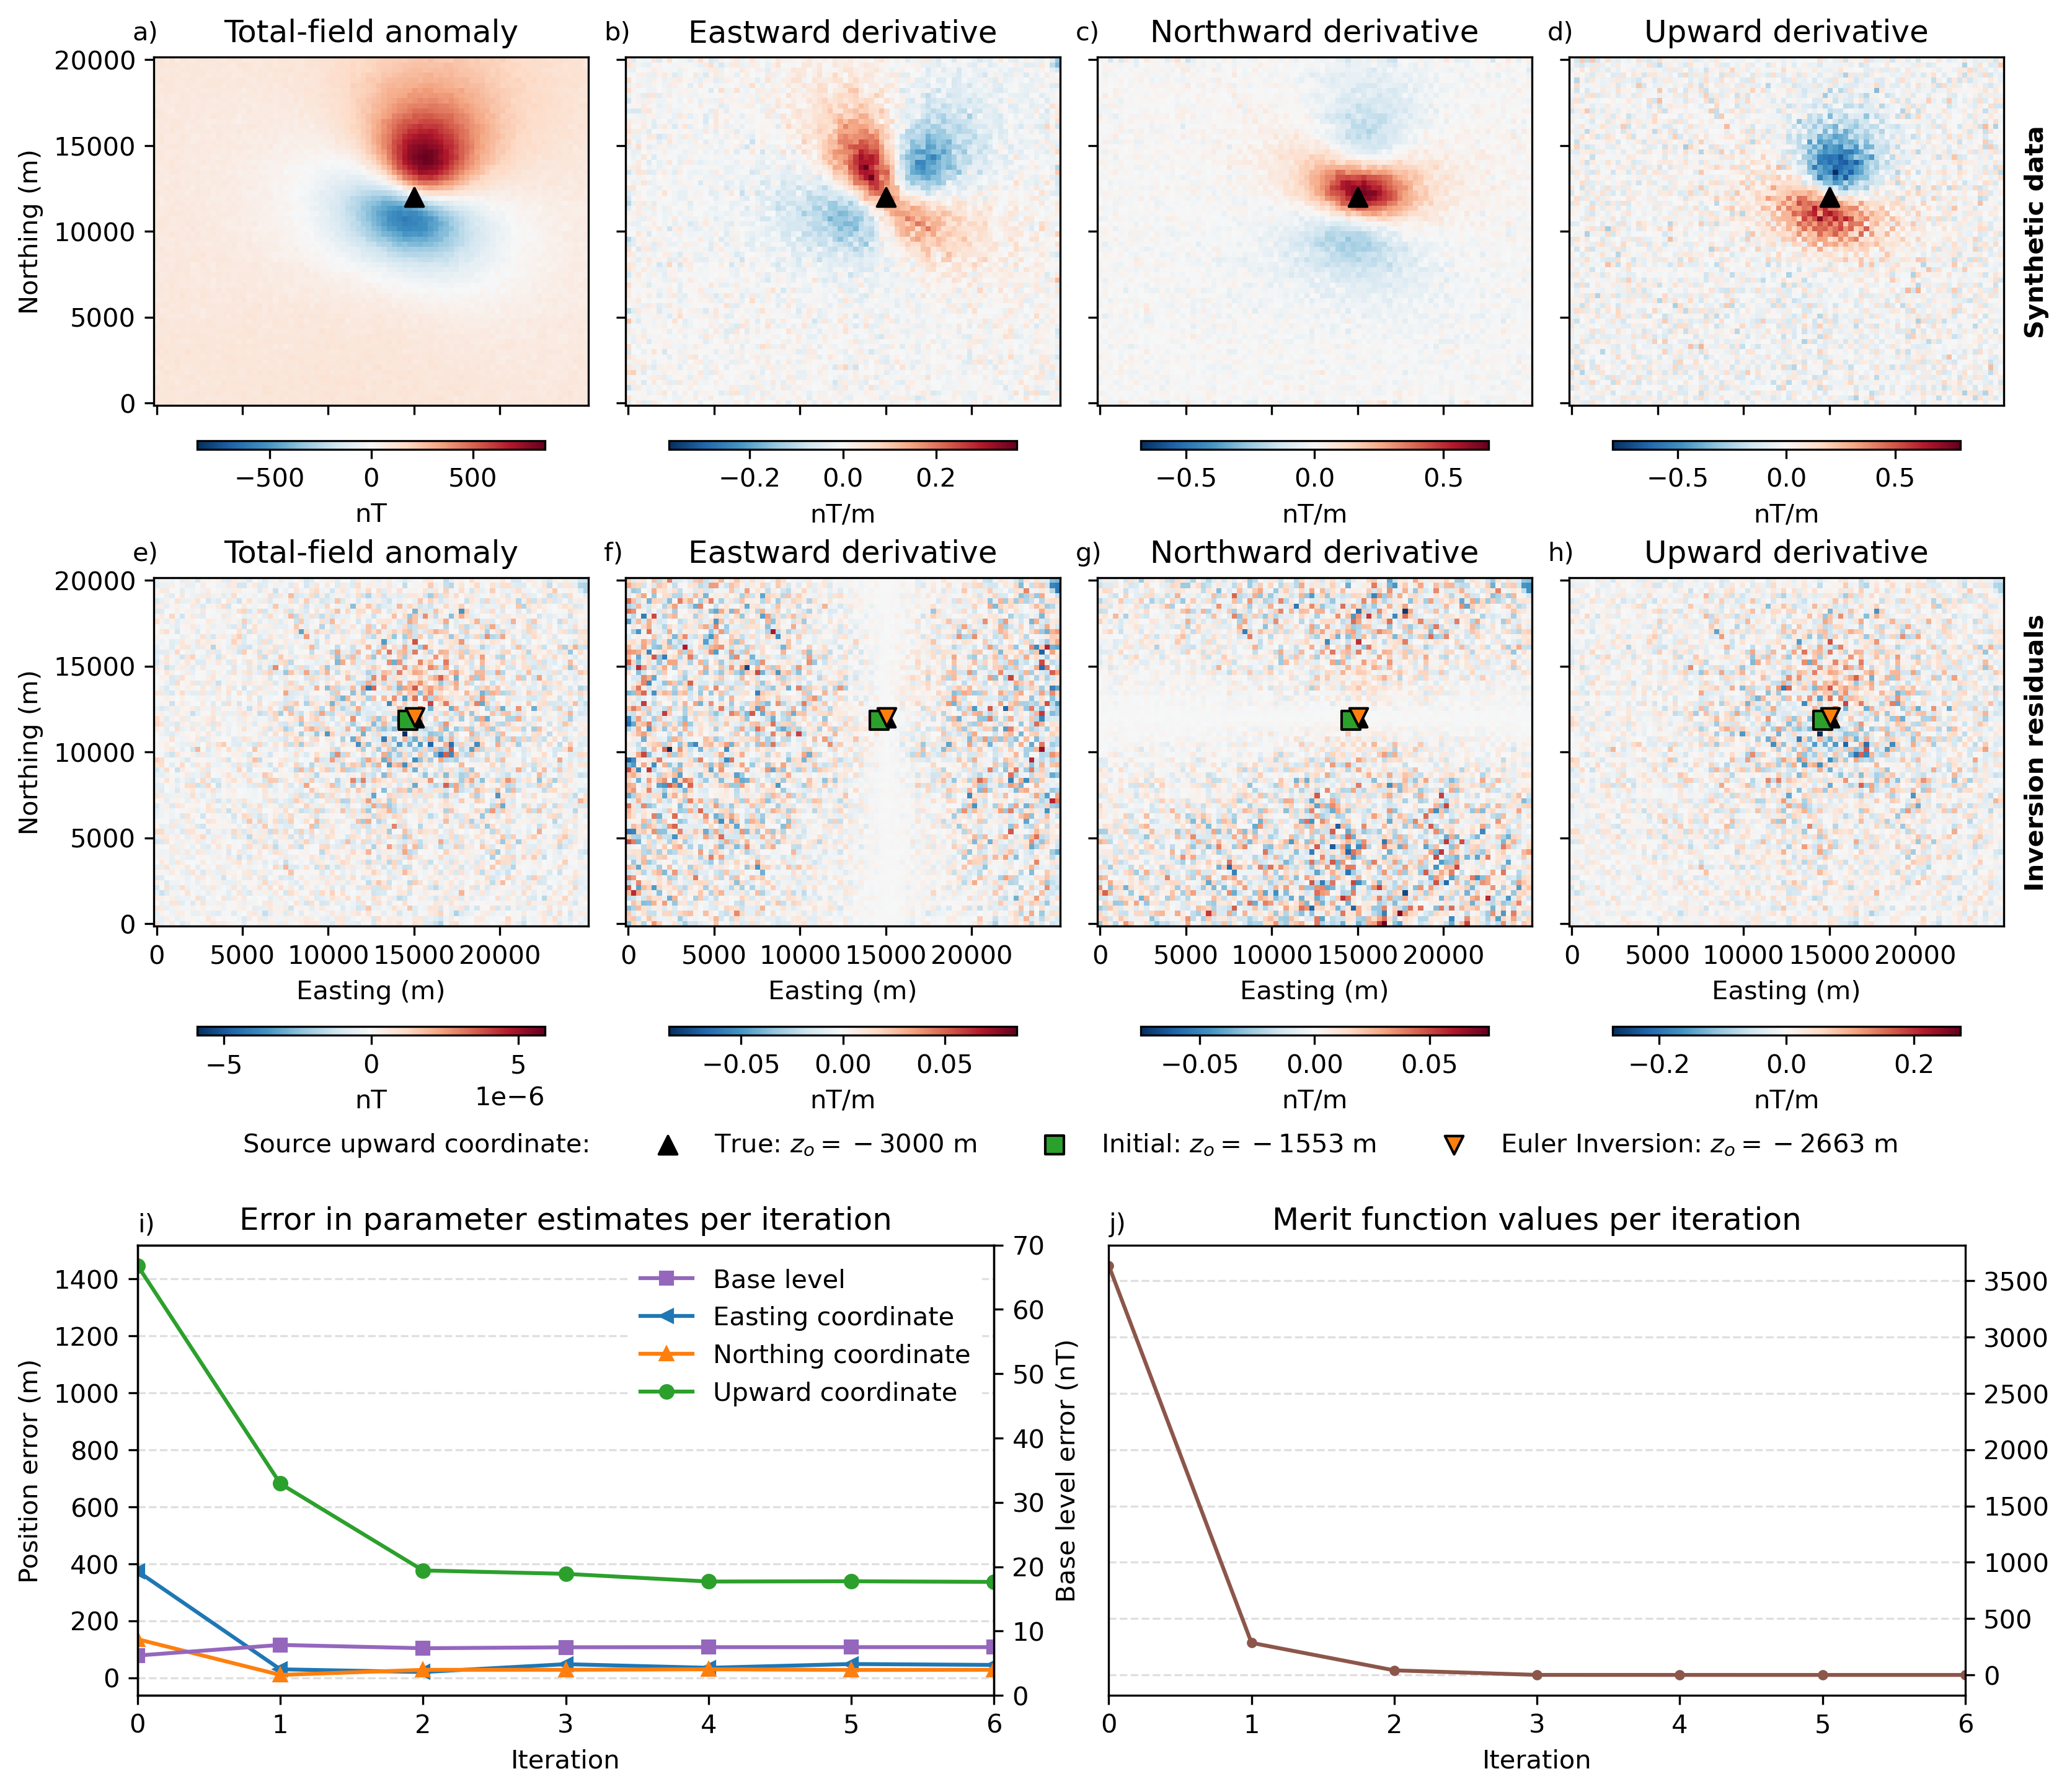
\includegraphics[width=1\linewidth]{euler-inversion/figures/synthetic-proof-of-concept.png}
\caption{
    Data and results from the synthetic data test to demonstrate the performance of the method on a single target.
    a-d) The noise-corrupted synthetic total-field anomaly and its eastward, northward, and upward derivatives, respectively. The position of the dipolar source is marked by the black triangle.
    e-h) The Euler inversion residuals (observed data minus predicted data) for the total-field anomaly and its easting, northing, and upward derivatives, respectively. The black triangle shows the true location of the source, the green square shows the location estimated by Euler deconvolution, and the orange triangle shows the location estimated by Euler inversion.
    i) The error in the estimate of the easting (blue line), northing (orange line), and upward (green line) coordinates of the source and the base level (purple line) as a function of the Gauss-Newton iteration (Algorithm~\ref{alg:ei}).
    j) The value of the merit function $\Merit$ (Equation~\ref{eq:merit}) per Gauss-Newton iteration.
}
\label{fig:proof}
\end{figure}

The main goal of this synthetic data test is to demonstrate the general effectiveness of the Euler inversion method to estimate the position and base level of a single source.
To this end, we created a model composed of a single dipole located at
$(x_o = \SynProofTrueEast, y_o = \SynProofTrueNorth, z_o = \SynProofTrueUp)$
with a dipole moment magnitude of \SynProofInt{}, inclination of \SynProofInc{}, and declination of \SynProofDec{}.
The reference field direction was the same as the dipole moment direction.
The synthetic total-field magnetic anomaly data was calculated on a regular grid
with point spacing of \SynProofSpacing{} at a height of \SynProofHeight{}.
To the data, we added a base level of \SynProofTrueBase{} and
pseudo-random Gaussian noise with \qty{0}{\nano\tesla} mean and \SynProofNoise{} standard deviation.
The eastward and northward derivatives of the total-field anomaly grid were calculated with a central-difference scheme.
The upward derivative was calculated by Fast Fourier Transform (FFT).
The synthetic anomaly and its three derivatives are shown in Figures~\ref{fig:proof}a-d.

The Euler inversion method described in Algorithm~\ref{alg:ei} was applied to the synthetic data.
We chose a fixed structural index of $\eta=3$, which is the correct index for a magnetic dipole.
For data weights, we used \DefaultWeightsF{} for the total-field anomaly, \DefaultWeightsE{} for the east-derivative, \DefaultWeightsN{} for the north-derivative, and \DefaultWeightsU{} for the upward-derivative.
These weights were chosen to counteract the increased effect of noise on the derivatives, particularly the upward derivative which was calculated through FFT.
Figures~\ref{fig:proof}e-h show the inversion residuals after convergence was achieved ($L=\SynProofNIter{}$ iterations) for the total-field anomaly and its eastward, northward, and upward derivatives, respectively.
Also shown are the true source location, the initial source location, and the predicted source location from Euler inversion.
The initial estimate of the source location was $(x_o=\SynProofEDEast,
y_o=\SynProofEDNorth, z_o=\SynProofEDUp)$ and the base level was $b
= \SynProofEDBase$, which are the Euler deconvolution results.
The final Euler inversion prediction of the source location was
$(x_o=\SynProofEstEast, y_o=\SynProofEstNorth, z_o=\SynProofEstUp)$ and the
estimated base level was $b = \SynProofEstBase$, which is an improvement on the
estimated values by Euler deconvolution (Figure~\ref{fig:proof}i).

Figure~\ref{fig:proof}i shows the error in the estimated source coordinates and base level.
We can see from the figure that the error in the $x_o$ (easting) and $y_o$
(northing) coordinates, as well as the base level, do not vary greatly from the
initial solution at iteration 0.
However, the error in the $z_o$ (upward) coordinate drops from over \qty{1400}{\m} to less than \qty{400}{\m} in two iterations.
The merit function (Equation~\ref{eq:merit}) also drops sharply in value by two iterations, as can be seen in Figure~\ref{fig:proof}j, confirming the rapid convergence of the Euler inversion method.


\subsection{Effect of structural index choice}
\label{sec:si}

\begin{figure}[tb!]
\centering
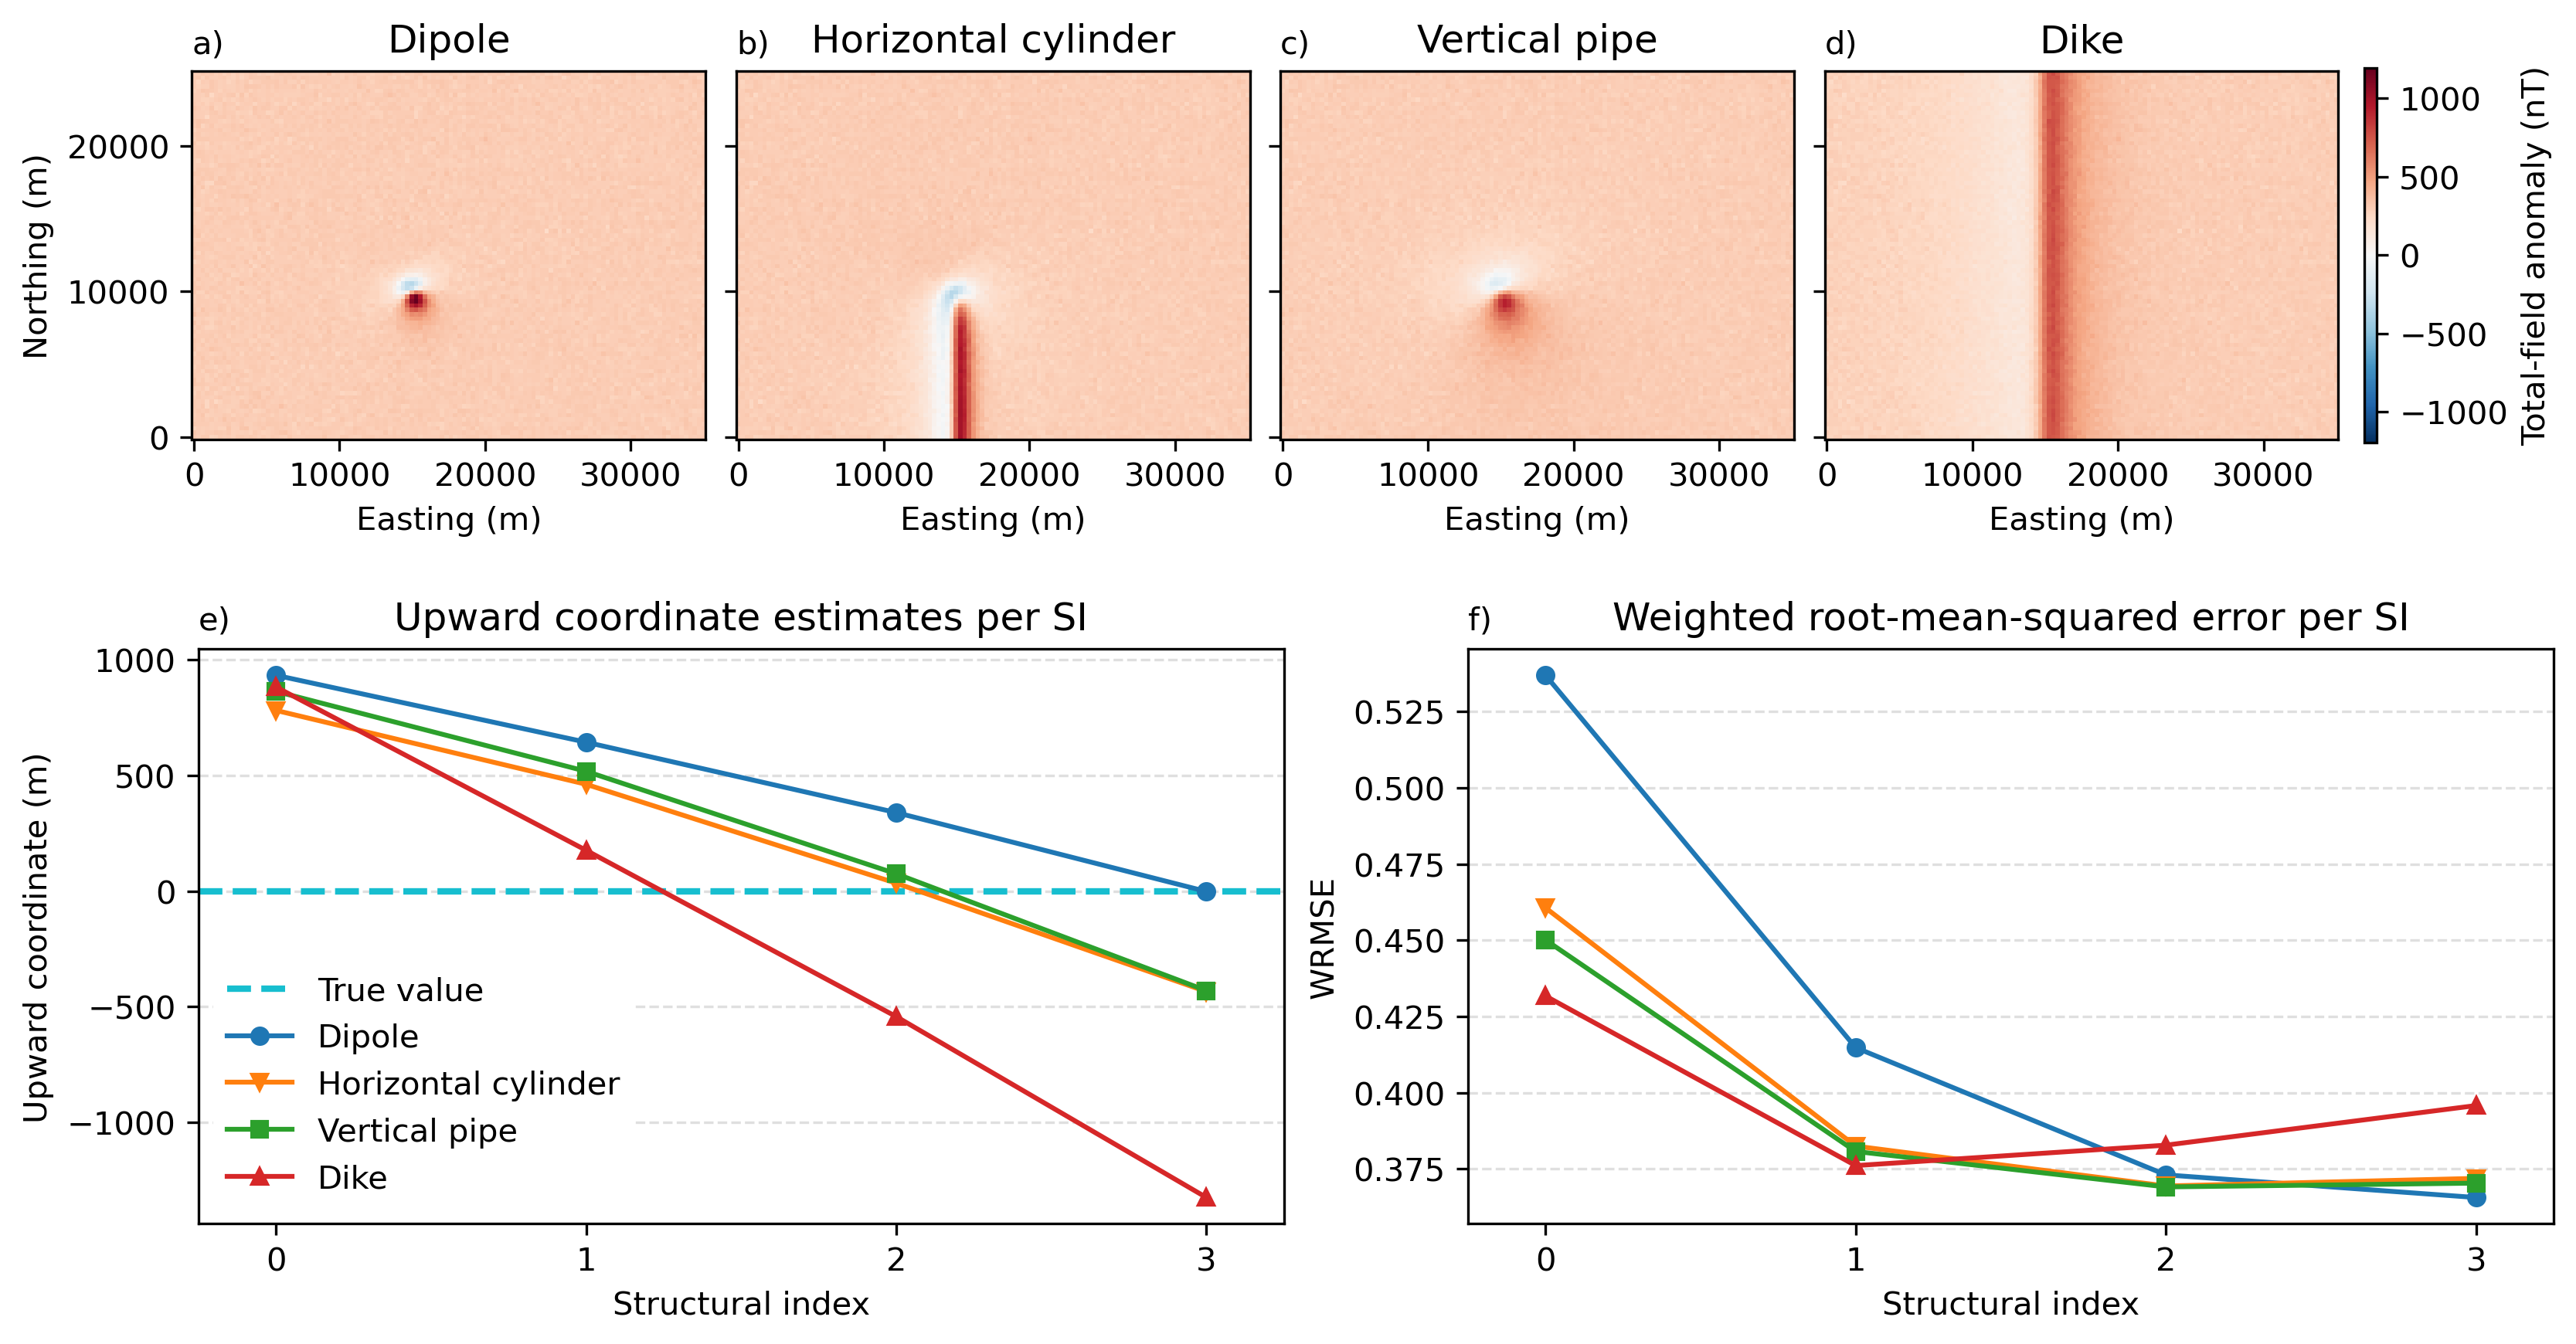
\includegraphics[width=1\linewidth]{euler-inversion/figures/synthetic-structural-index.png}
\caption{
    Data and results from the synthetic data test using different values of structural index $\eta$ for different source types.
    a-d) Noise-corrupted total-field magnetic anomaly data caused by a dipole ($\eta=3$), a horizontal cylinder ($\eta=2$), a vertical pipe ($\eta=2$), and a vertical North-South dyke ($\eta=1$), respectively.
    e) Estimate of the upward source coordinate $z_o$ as a function of structural index for the dipole (blue line), horizontal cylinder (orange line), vertical pipe (green line), and dyke (red line).
    The true upward coordinate of the sources ($z_o = \SynSITrueUp$) is marked by the blue dashed line. Note that the $z_o$ estimate is closest to the true value when the correct structural index for each source type is used.
    f) The weighted root-mean-squared error (WRMSE; Equation~\ref{eq:wrmse}) as a function of structural index for the dipole (blue line), horizontal cylinder (orange line), vertical pipe (green line), and dyke (red line). The WRMSE is minimum for each source type when the correct structural index is used.
}
\label{fig:si}
\end{figure}

In this synthetic data test, we created datasets using four different models: a dipole, a horizontal cylinder composed of a right-rectangular prism stretched in the southward direction, a vertical pipe composed of a right-rectangular prism stretched in the downward direction, and a vertical dyke composed of a right-rectangular prism stretched in the southward, northward, and downward directions.
All models share the same true location of $(x_o=\SynSITrueEast, y_o=\SynSITrueNorth, z_o=\SynSITrueUp)$, base level of \SynSITrueBase, and induced magnetisation with inclination of \SynSIInc{} and declination of \SynSIDec.
The data were generated on a regular grid with spacing of \SynSISpacing, height of \SynSIHeight, and contaminated with pseudo-random Gaussian noise with \qty{0}{\nano\tesla} mean and \SynSINoise{} standard deviation. Figures~\ref{fig:si}a-d show the synthetic noise-corrupted total-field anomaly data.

We ran the Euler inversion method on each data grid four times, each time
changing the structural index between zero, one, two, and three.
Figure~\ref{fig:si}e shows the upward coordinate $z_o$ estimated for each of the four models as a function of the structural index $\eta$.
The Euler inversion estimated $z_o$ correlates with $\eta$, with larger values of the structural index leading to deeper source estimates.
Values closest to the true $z_o=\SynSITrueUp$ are achieved when the correct structural index is used ($\eta=1$ for the dyke, $\eta=2$ for the cylinder and pipe, and $\eta=3$ for the dipole).
Figure~\ref{fig:si}f shows the weighted root-mean-squared error (WRMSE; Equation~\ref{eq:wrmse}) at the final iteration of the Euler inversion method for all four models as a function of structural index.
The WRMSE is a measure of goodness-of-fit between the predicted total-field anomaly and its three derivatives and their observed counterparts.
The WRMSE is minimum for all four models when the correct structural index is used.


\subsection{Effect of random noise}
\label{sec:noise}

\begin{figure}[tb!]
\centering
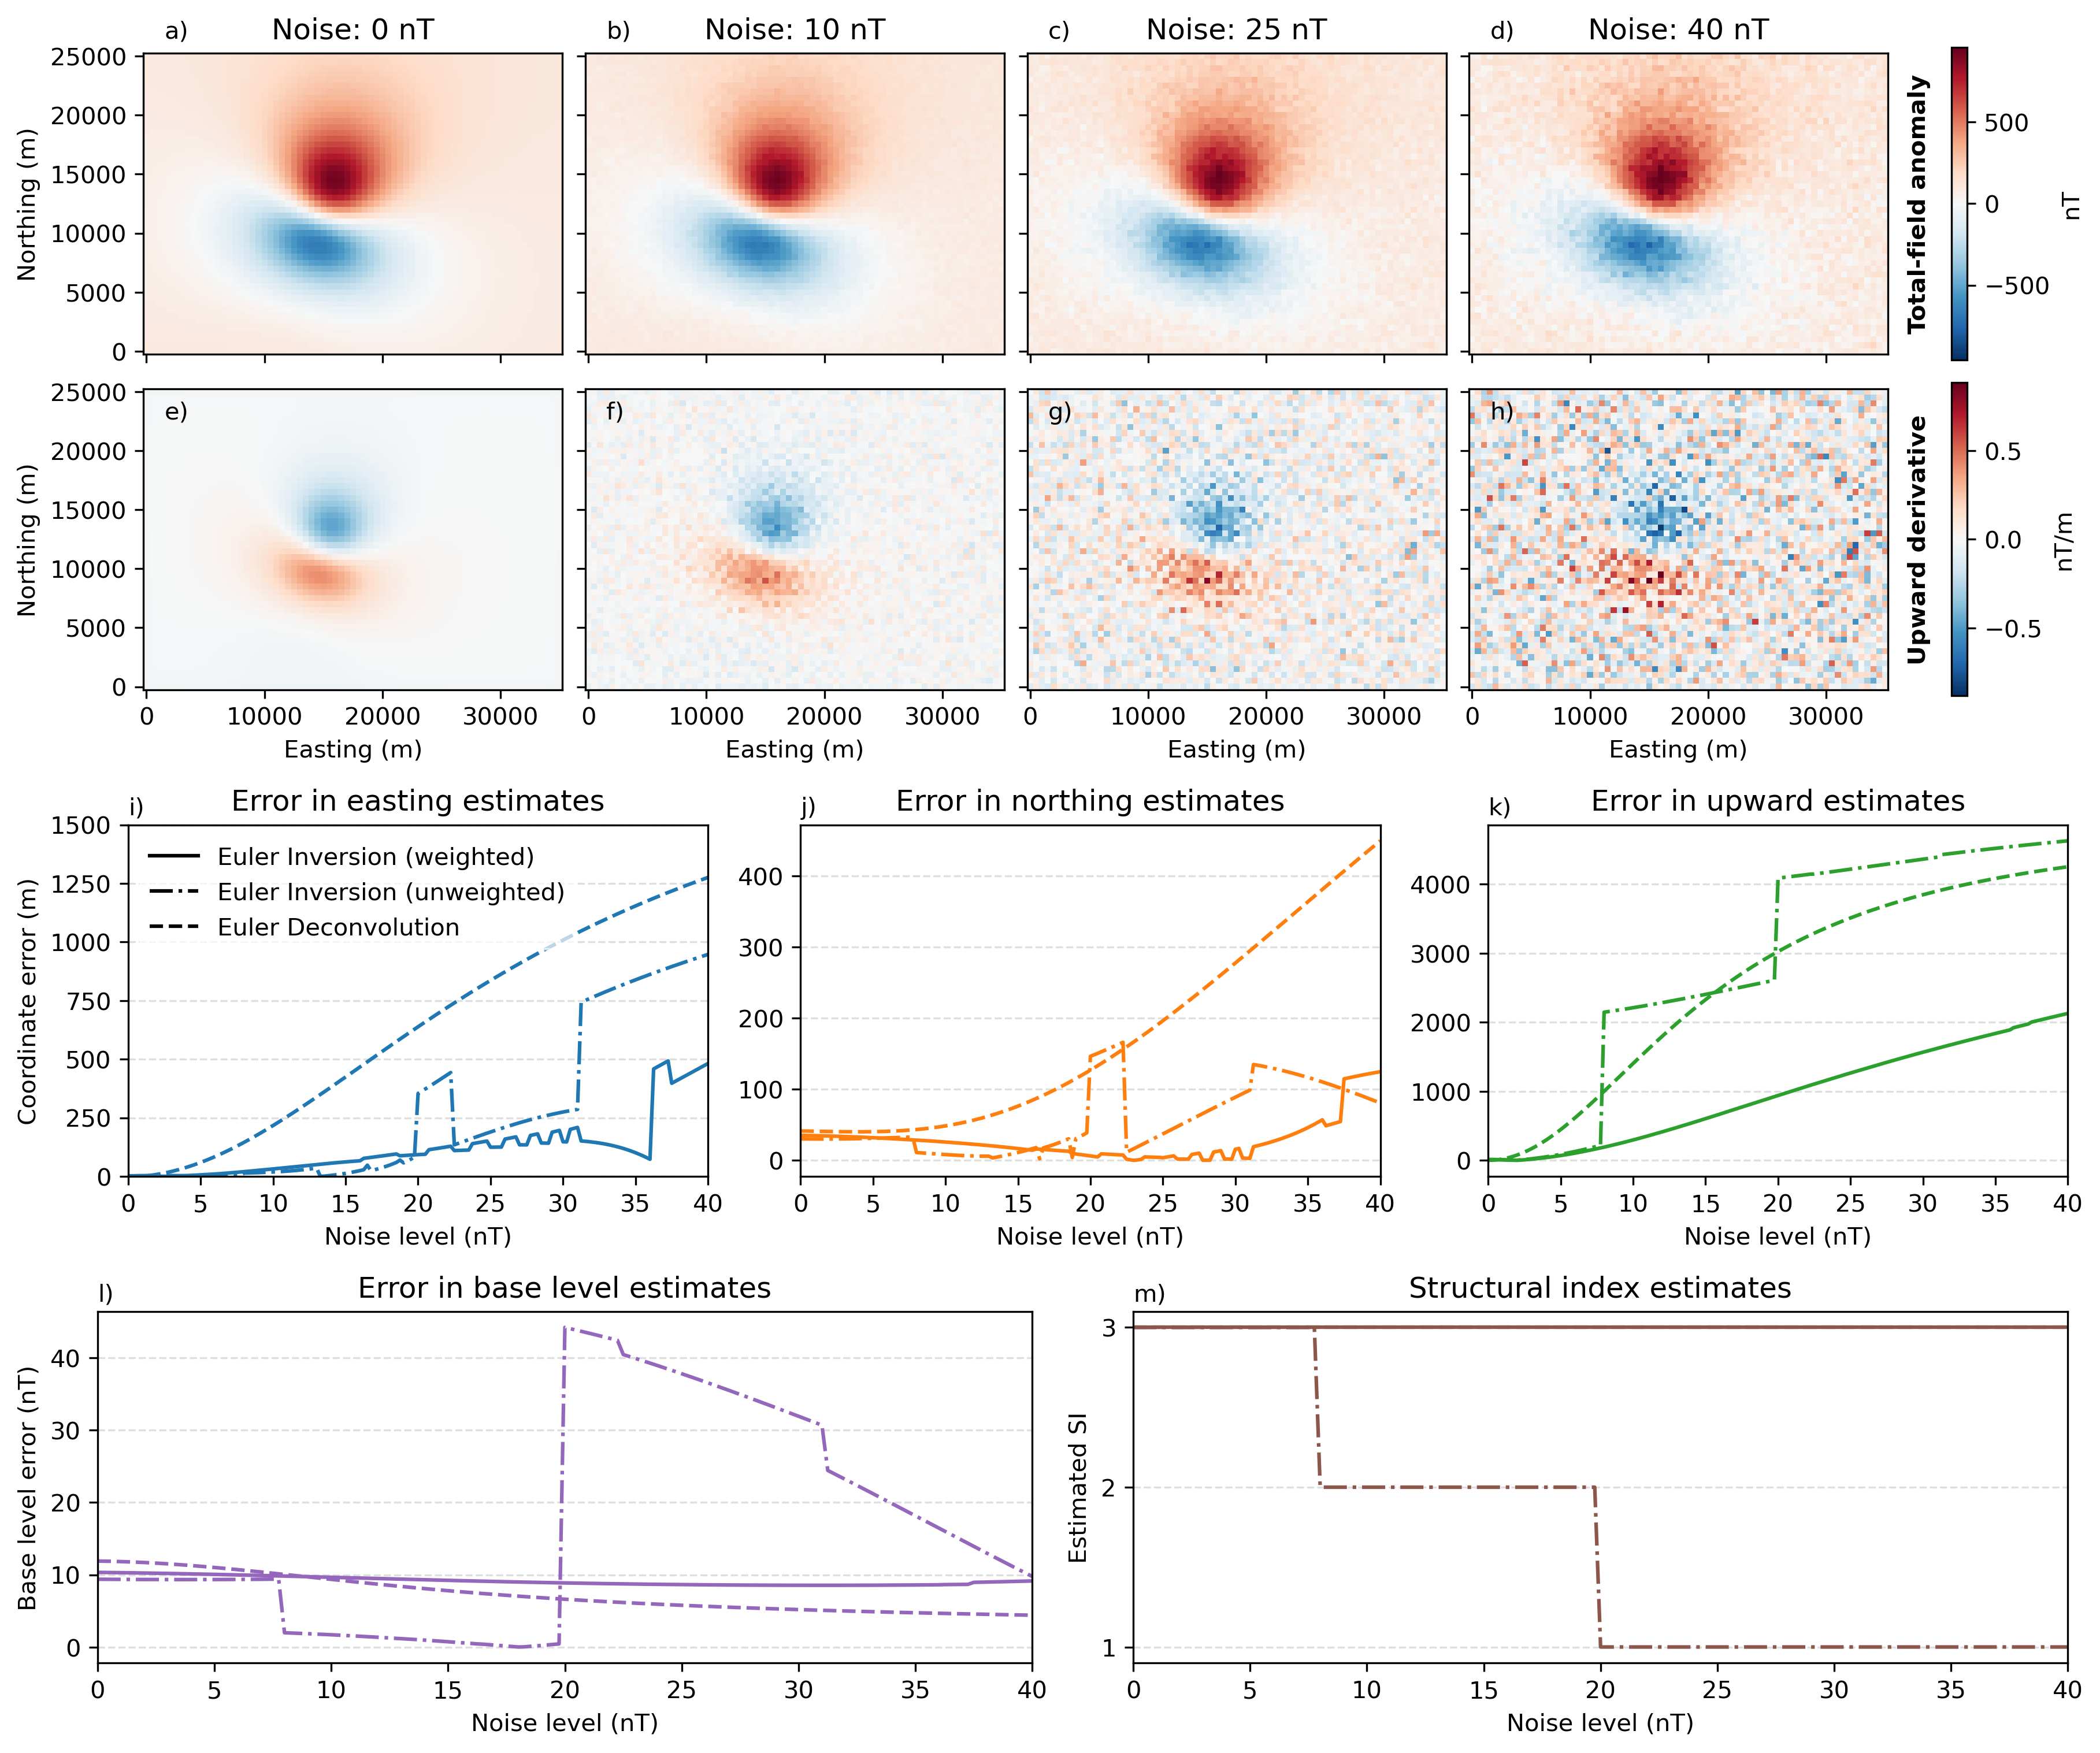
\includegraphics[width=1\linewidth]{euler-inversion/figures/synthetic-noise-levels.png}
\caption{
    Data and results from the synthetic data test used to investigate the effect of high-frequency noise on the Euler inversion results.
    a-d) Noise-corrupted total-field magnetic anomaly of a dipolar source for noise levels \SynNoisePlotted.
    e-h) The upward derivative of the data in a-d, calculated by FFT.
    i-k) Error in the estimated easting, northing, and upward coordinates, respectively.
    l) Error in the estimated base level.
    m) The estimated structural index $\eta$ using Algorithm~\ref{alg:si}.
    The lines in i-m are the results for Euler deconvolution (dashed line), Euler inversion without data weights (dashed-dotted line), and Euler inversion with weights (solid line) \SynNoiseWeightsF{} for the total-field anomaly, \SynNoiseWeightsE{} for the eastward derivative, \SynNoiseWeightsN{} for the northward derivative, and \SynNoiseWeightsU{} for the upward derivative.
}
\label{fig:noise}
\end{figure}

We conducted another experiment to determine the effect of random high-frequency noise on the Euler inversion estimates.
To this end, we created synthetic data from a dipole model located at $(x_o=\SynNoiseTrueEast, y_o=\SynNoiseTrueNorth, z_o=\SynNoiseTrueUp)$ and with a dipole moment magnitude of \SynNoiseInt{}, inclination of \SynNoiseInc, and declination of \SynNoiseDec.
The total-field anomaly data were generated on a regular grid with a spacing of \SynNoiseSpacing{} and a constant height of \SynNoiseHeight.
The reference field direction was the same as the dipole moment direction.
A base level of \SynNoiseTrueBase{} was added to the data.
We generated different datasets by adding pseudo-random Gaussian noise with \qty{0}{\nano\tesla} mean and standard deviations varying from \SynNoiseMin{} to \SynNoiseMax{} with a step of \SynNoiseStep{}.
Figures~\ref{fig:noise}a-d show the synthetic data for noise levels \SynNoisePlotted, while Figures~\ref{fig:noise}e-h show the upward derivative calculated from the total-field anomaly through FFT.

On each dataset, we ran Euler deconvolution (Equation~\ref{eq:deconv-p}), Euler inversion with unit weights, and Euler inversion with weights \SynNoiseWeightsF{} for the total-field anomaly, \SynNoiseWeightsE{} for the eastward derivative, \SynNoiseWeightsN{} for the northward derivative, and \SynNoiseWeightsU{} for the upward derivative.
Both Euler inversion runs used the structural index estimation procedure
(Algorithm~\ref{alg:si} with $\eta_{min}=\DefaultSIMin$ and
$\eta_{max}=\DefaultSIMax$).
Figures~\ref{fig:si}i-l show the error in the estimated easting, northing, and upward coordinates as well as the base level for each of the methods as a function of noise level.
The error in each of three coordinates raises sharply with noise level for Euler deconvolution, particularly for the upward $z_o$ coordinate.
The unweighted Euler inversion results vary less regularly but the present errors are just as large as Euler deconvolution for the upward coordinate.
However, the weighted Euler inversion presented overall smaller errors and a slower growth curve for the upward coordinate error than the other two methods.
The base level error is nearly constant at approximately \qty{10}{\nano\tesla} for Euler deconvolution and the weighted Euler inversion, but varies to as much as \qty{40}{\nano\tesla} for the unweighted Euler inversion.

Figure~\ref{fig:noise}m shows the estimated structural index $\eta$ for the weighted and unweighted Euler inversion as a function of noise level.
The unweighted Euler inversion estimated the wrong structural index $\eta=2$ from approximately noise level \qty{7}{\nano\tesla} and $\eta=1$ from approximately noise level \qty{20}{\nano\tesla}.
These jumps in the estimated structural index appear to correlate with jumps in the base level and $z_o$ coordinate errors.
The weighted Euler inversion was able to estimate the correct structural index ($\eta=3$) for all noise levels tested.


\subsection{Effect of interfering sources}
\label{sec:interf}

\begin{figure}[tb!]
\centering
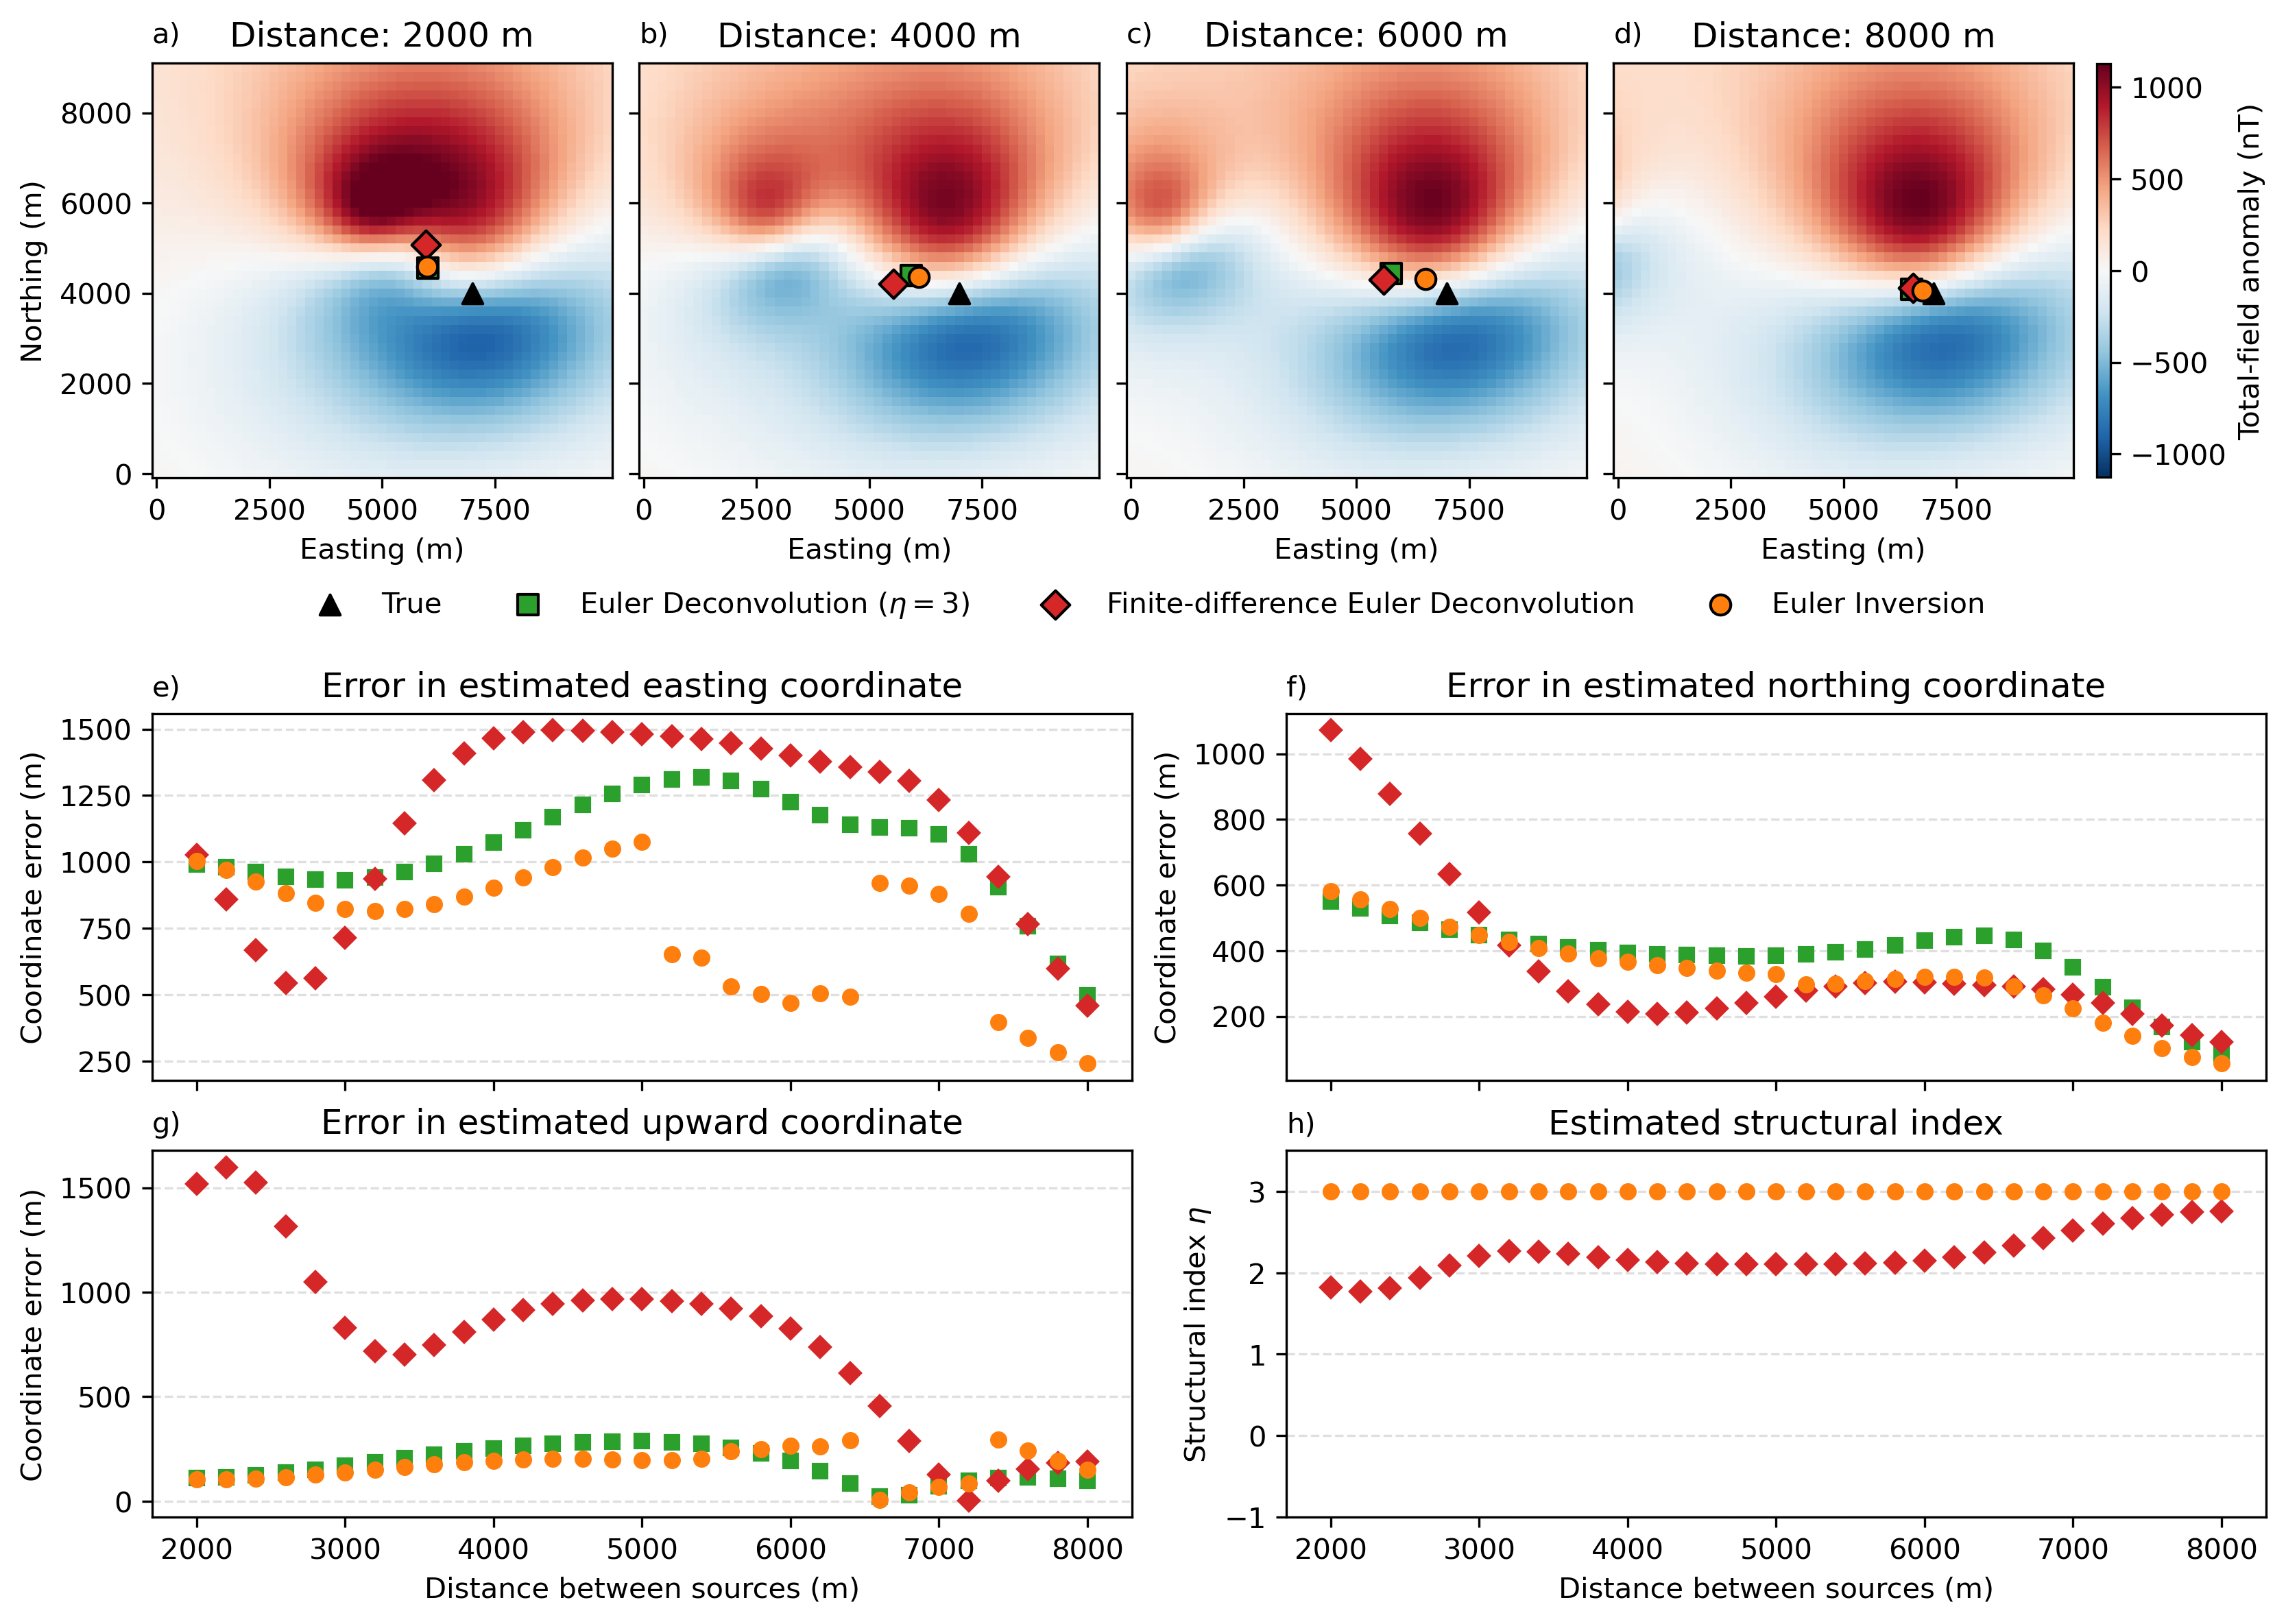
\includegraphics[width=1\linewidth]{euler-inversion/figures/synthetic-interfering-sources.png}
\caption{
    Data and results from the synthetic data test used to investigate the
    effect of interfering dipolar sources inside the data window on the Euler
    inversion results.
    a-d) Total-field magnetic anomaly of four out of the \SynInterfNModels{}
    models, each of which includes the same central dipole and an interfering
    dipolar source at different distances from the main source. Also plotted
    are the estimated positions from Euler deconvolution (green square),
    finite-difference Euler deconvolution (red diamond), and Euler inversion
    (orange circle).
    e-g) The error in the estimated eastward, northward, and upward
    coordinates, respectively, of the source for each of the Euler methods as
    a function of the distance between sources.
    h) The estimated structural index $\eta$ for Euler inversion and
    finite-difference Euler deconvolution as a function of the distance between
    sources.
}
\label{fig:interf}
\end{figure}

\begin{figure}[tb!]
\centering
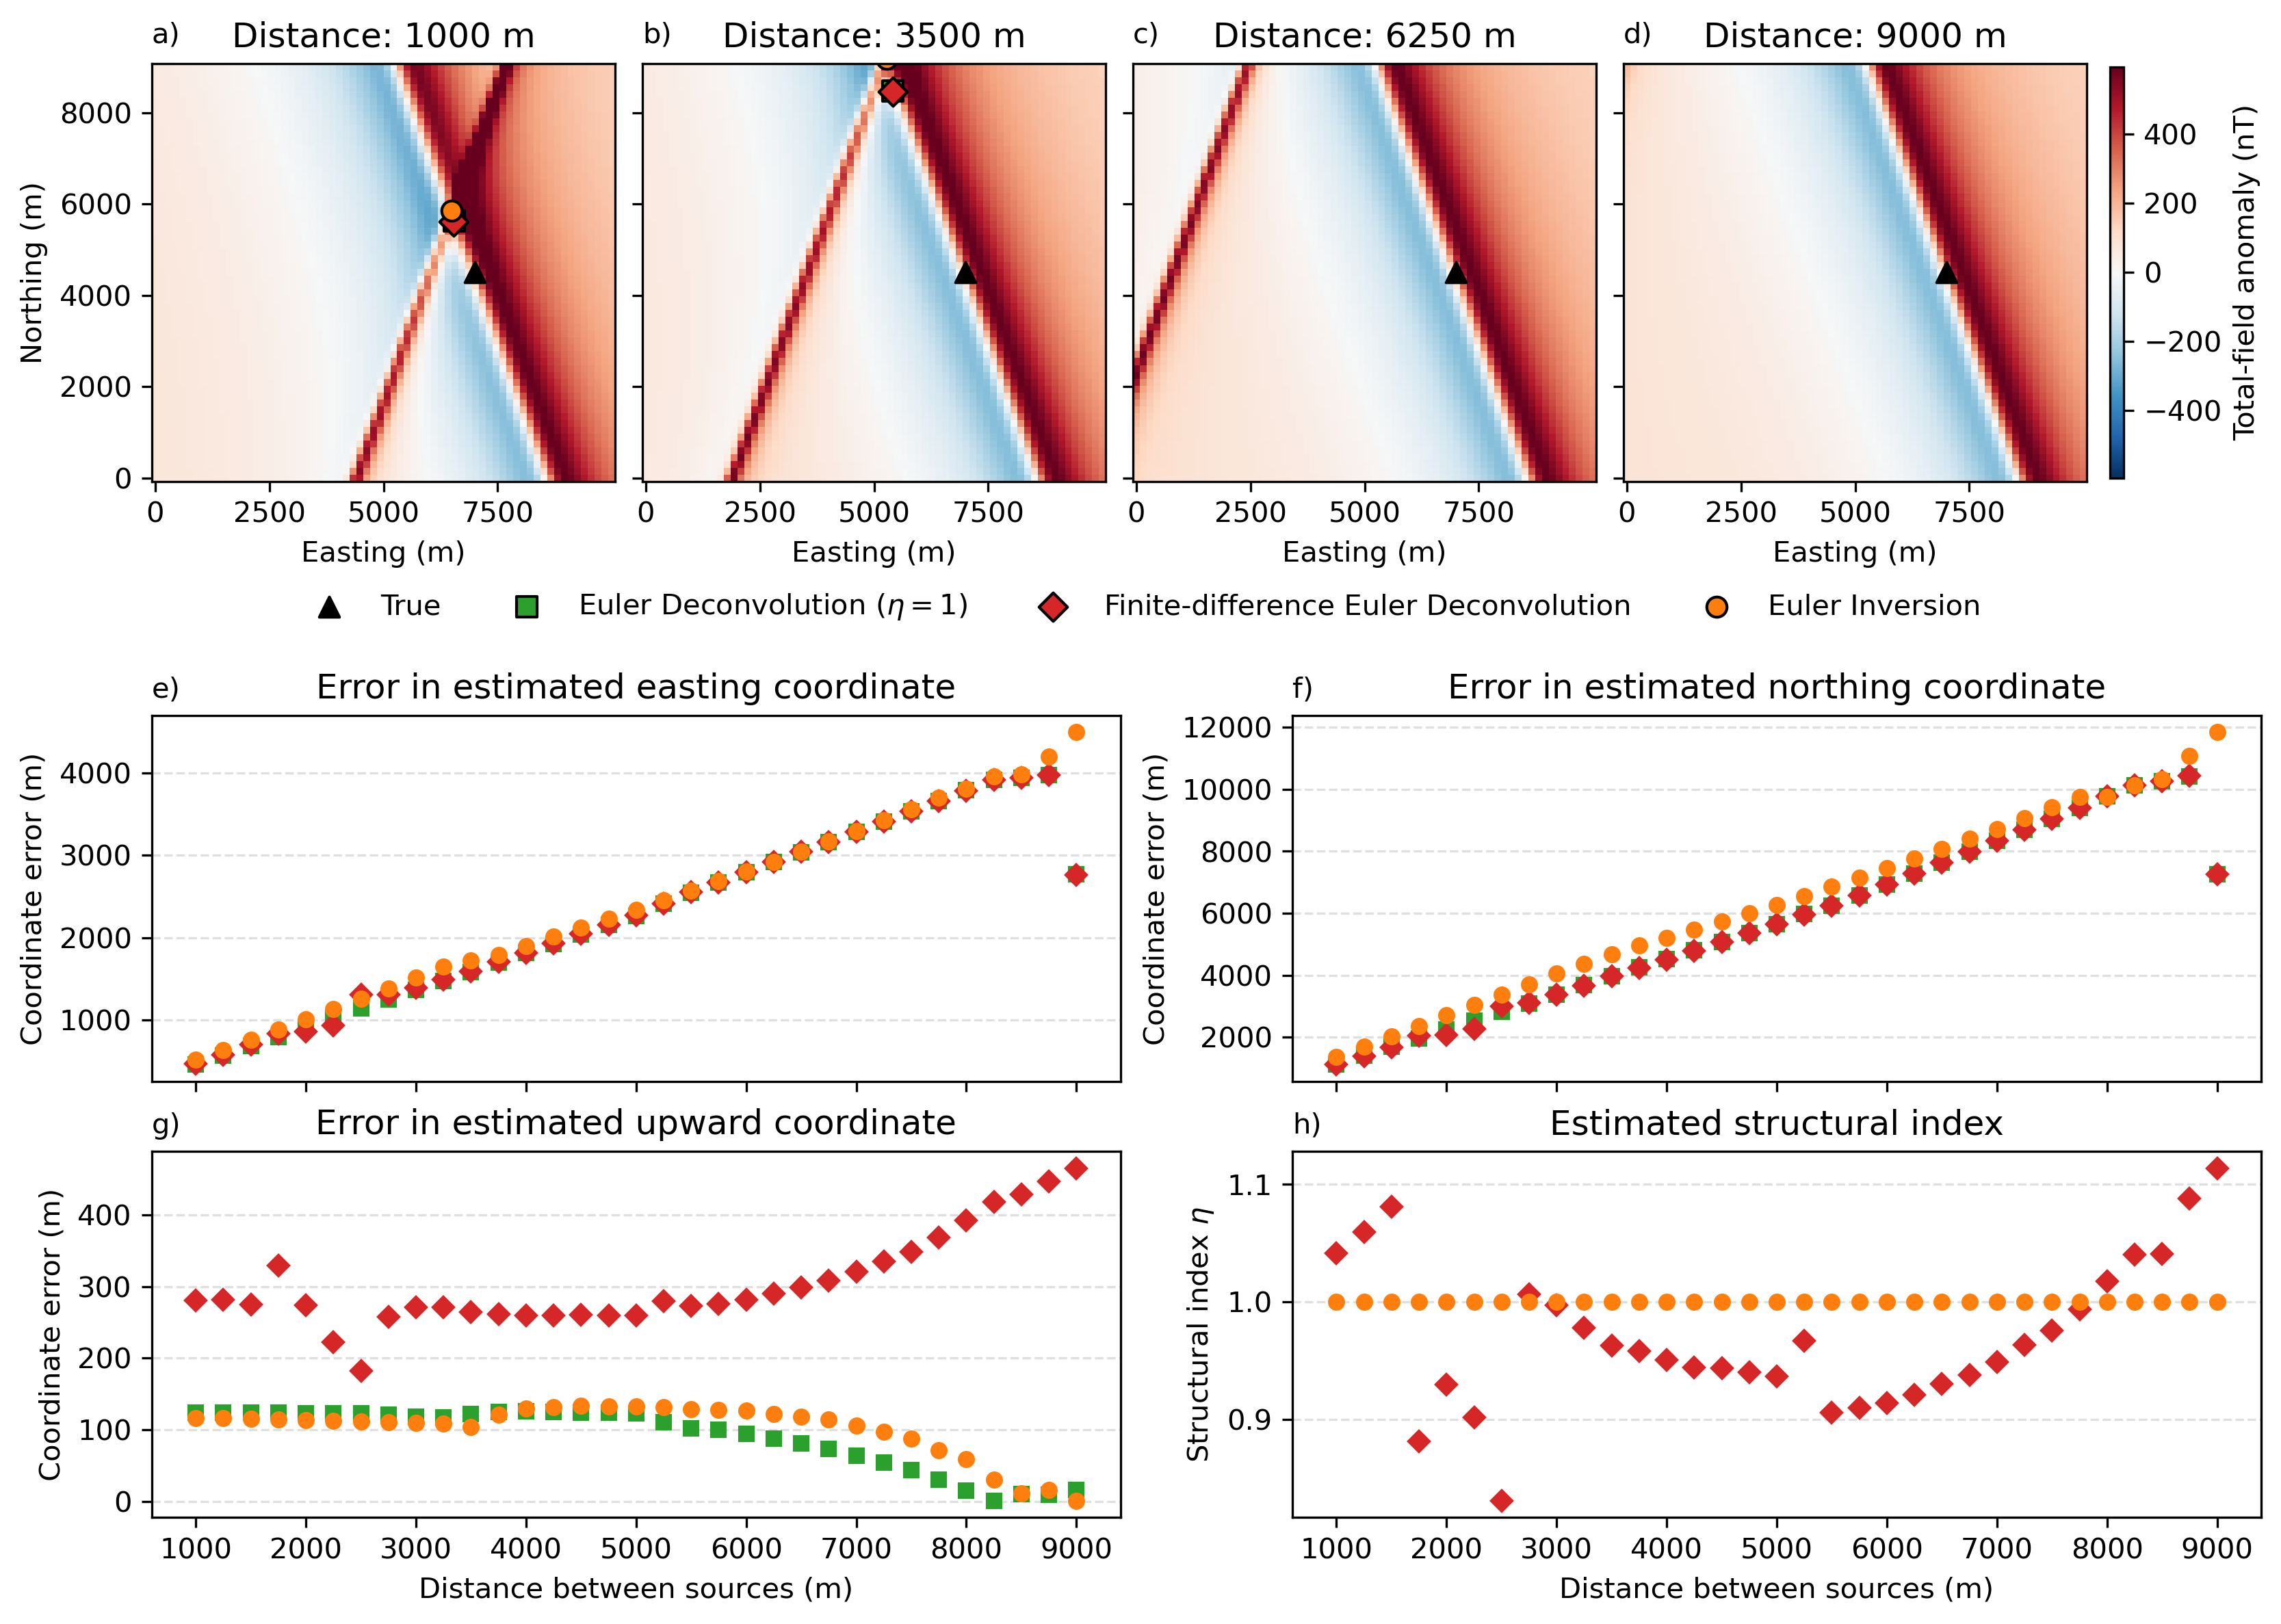
\includegraphics[width=1\linewidth]{euler-inversion/figures/synthetic-interfering-sources-dykes.png}
\caption{
    Data and results from the synthetic data test used to investigate the
    effect of interfering dykes inside the data window on the Euler inversion
    results.
    a-d) Total-field magnetic anomaly of four out of the \SynInterfDykesNModels{}
    models, each of which includes the same dyke to the east and an interfering
    dyke to the west at different distances from the main source. Also plotted
    are the estimated positions from Euler deconvolution (green square),
    finite-difference Euler deconvolution (red diamond), and Euler inversion
    (orange circle).
    In c and d, the three Euler solutions are not visible because they are
    outside the data window.
    e-g) The error in the estimated eastward, northward, and upward
    coordinates, respectively, of the source for each of the Euler methods as
    a function of the distance between sources. The error for the eastward and
    northward coordinates was calculated with respect to the center point of
    the eastern dyke (black triangle).
    h) The estimated structural index $\eta$ for Euler inversion and
    finite-difference Euler deconvolution as a function of the distance between
    sources.
}
\label{fig:interf-dykes}
\end{figure}

Another common issue encountered during the application of Euler-based methods
is the presence of interfering sources within the data window.
To test this effect on Euler inversion, we create two different scenarios, one
with two dipoles and another with two dykes.
In both scenarios, we created several synthetic total-field anomaly datasets
by varying the distance between the two sources.
No noise was added to these synthetic data in order to isolate the effect of
the interfering source from the effect of random noise.
We added to all datasets a base level of \SynInterfTrueBase{}.
On each dataset, we ran Euler deconvolution (Equation~\ref{eq:deconv-p}) with
the correct structural index for the source ($\eta=3$ for the dipoles and
$\eta=1$ for the dykes), the finite-difference Euler deconvolution method of
\citet{Gerovska2005}, and Euler inversion with the structural index estimation
(Algorithm~\ref{alg:si} with $\eta_{min}=\DefaultSIMin$ and
$\eta_{max}=\DefaultSIMax$) and data weights of \DefaultWeightsF{} for the
total-field anomaly, \DefaultWeightsE{} for the eastward derivative,
\DefaultWeightsN{} for the northward derivative, and \DefaultWeightsU{} for the
upward derivative.

The dipole models contain a main dipole located at $(x_o=\SynInterfTrueEast,
y_o=\SynInterfTrueNorth, z_o=\SynInterfTrueUp)$ with a dipole moment amplitude
of \SynInterfInt{}, inclination of \SynInterfInc, and declination of
\SynInterfDec.
The interfering dipole was located at $y_o=\SynInterfInterfNorth$ and
$z_o=\SynInterfInterfUp$, with the $x_o$ coordinate varying from
\SynInterfInterfEastMin{} to \SynInterfInterfEastMax{}.
The reference field direction was the same as the dipole moment direction.
The total-field anomaly data were generated on regular grids with a spacing of
\SynInterfSpacing{} and at a constant height of \SynInterfHeight.
Figures~\ref{fig:interf}a-d show the total-field anomaly of four out of the
\SynInterfNModels{} models.

The error in the estimated eastward, northward, and upward coordinates are
shown in Figures~\ref{fig:interf}e-g.
For the eastward and northward coordinates, the three methods are mostly
compatible, with Euler inversion being slightly closer to the true source for
most distances between sources.
For the upward coordinate, Euler inversion and Euler deconvolution are
roughly equivalent and both have smaller errors than finite-difference Euler
deconvolution for all but the largest distances.
For the structural index estimates (Figure~\ref{fig:interf}h),
finite-difference Euler deconvolution underestimates $\eta$ for all but the
largest distances, while Euler inversion estimates the correct index of
$\eta=3$ for all distances.

The dyke models contain a main dyke at the east with a center point at
$(x_o=\SynInterfDykesTrueEast, y_o=\SynInterfDykesTrueNorth)$ and a top at
$z_o=\SynInterfDykesTrueUp$ with a dipole moment amplitude
of \SynInterfDykesInt{}, inclination of \SynInterfDykesInc, and declination of
\SynInterfDykesDec.
The interfering dyke has a top at $z_o=\SynInterfDykesInterfUp$, with the $x_o$
coordinate varying from
\SynInterfDykesInterfEastMin{} to \SynInterfDykesInterfEastMax{}.
The reference field direction was the same as the dipole moment direction.
The total-field anomaly data were generated on regular grids with a spacing of
\SynInterfDykesSpacing{} and at a constant height of \SynInterfDykesHeight.
Figures~\ref{fig:interf-dykes}a-d show the total-field anomaly of four out of
the \SynInterfDykesNModels{} models.

The error in the estimated eastward, northward, and upward coordinates are
shown in Figures~\ref{fig:interf-dykes}e-g.
The error for the eastward and northward coordinates was calculated with
respect to the center point of the eastern dyke.
For the eastward and northward coordinates, the three methods are mostly
compatible.
When the two dykes intersect, all three methods estimate a horizontal position
at the intersection point.
When they don't intersect, the estimates for all three methods falls outside of
the data window.
This is a well known issue for Euler deconvolution methods because the Hessian
matrix $\mathbf{A}^T\mathbf{A}$ (Equation~\ref{eq:deconv-p}) is ill-conditioned
for 2D sources \citep{Mushayandebvu2004}.
For the upward coordinate, Euler inversion and Euler deconvolution are
roughly equivalent and approach zero at the largest distances.
Both methods have smaller errors than finite-difference Euler deconvolution for
all distances tested.
For the structural index estimates (Figure~\ref{fig:interf-dykes}h),
finite-difference Euler deconvolution estimates incorrect $\eta$ at most
distances, presenting no clear relationship between distance and $\eta$
estimate.
Euler inversion estimates the correct index of $\eta=1$ for all distances.


\subsection{Moving window procedure with multiple sources}
\label{sec:windows}

\begin{figure}[tb!]
\centering
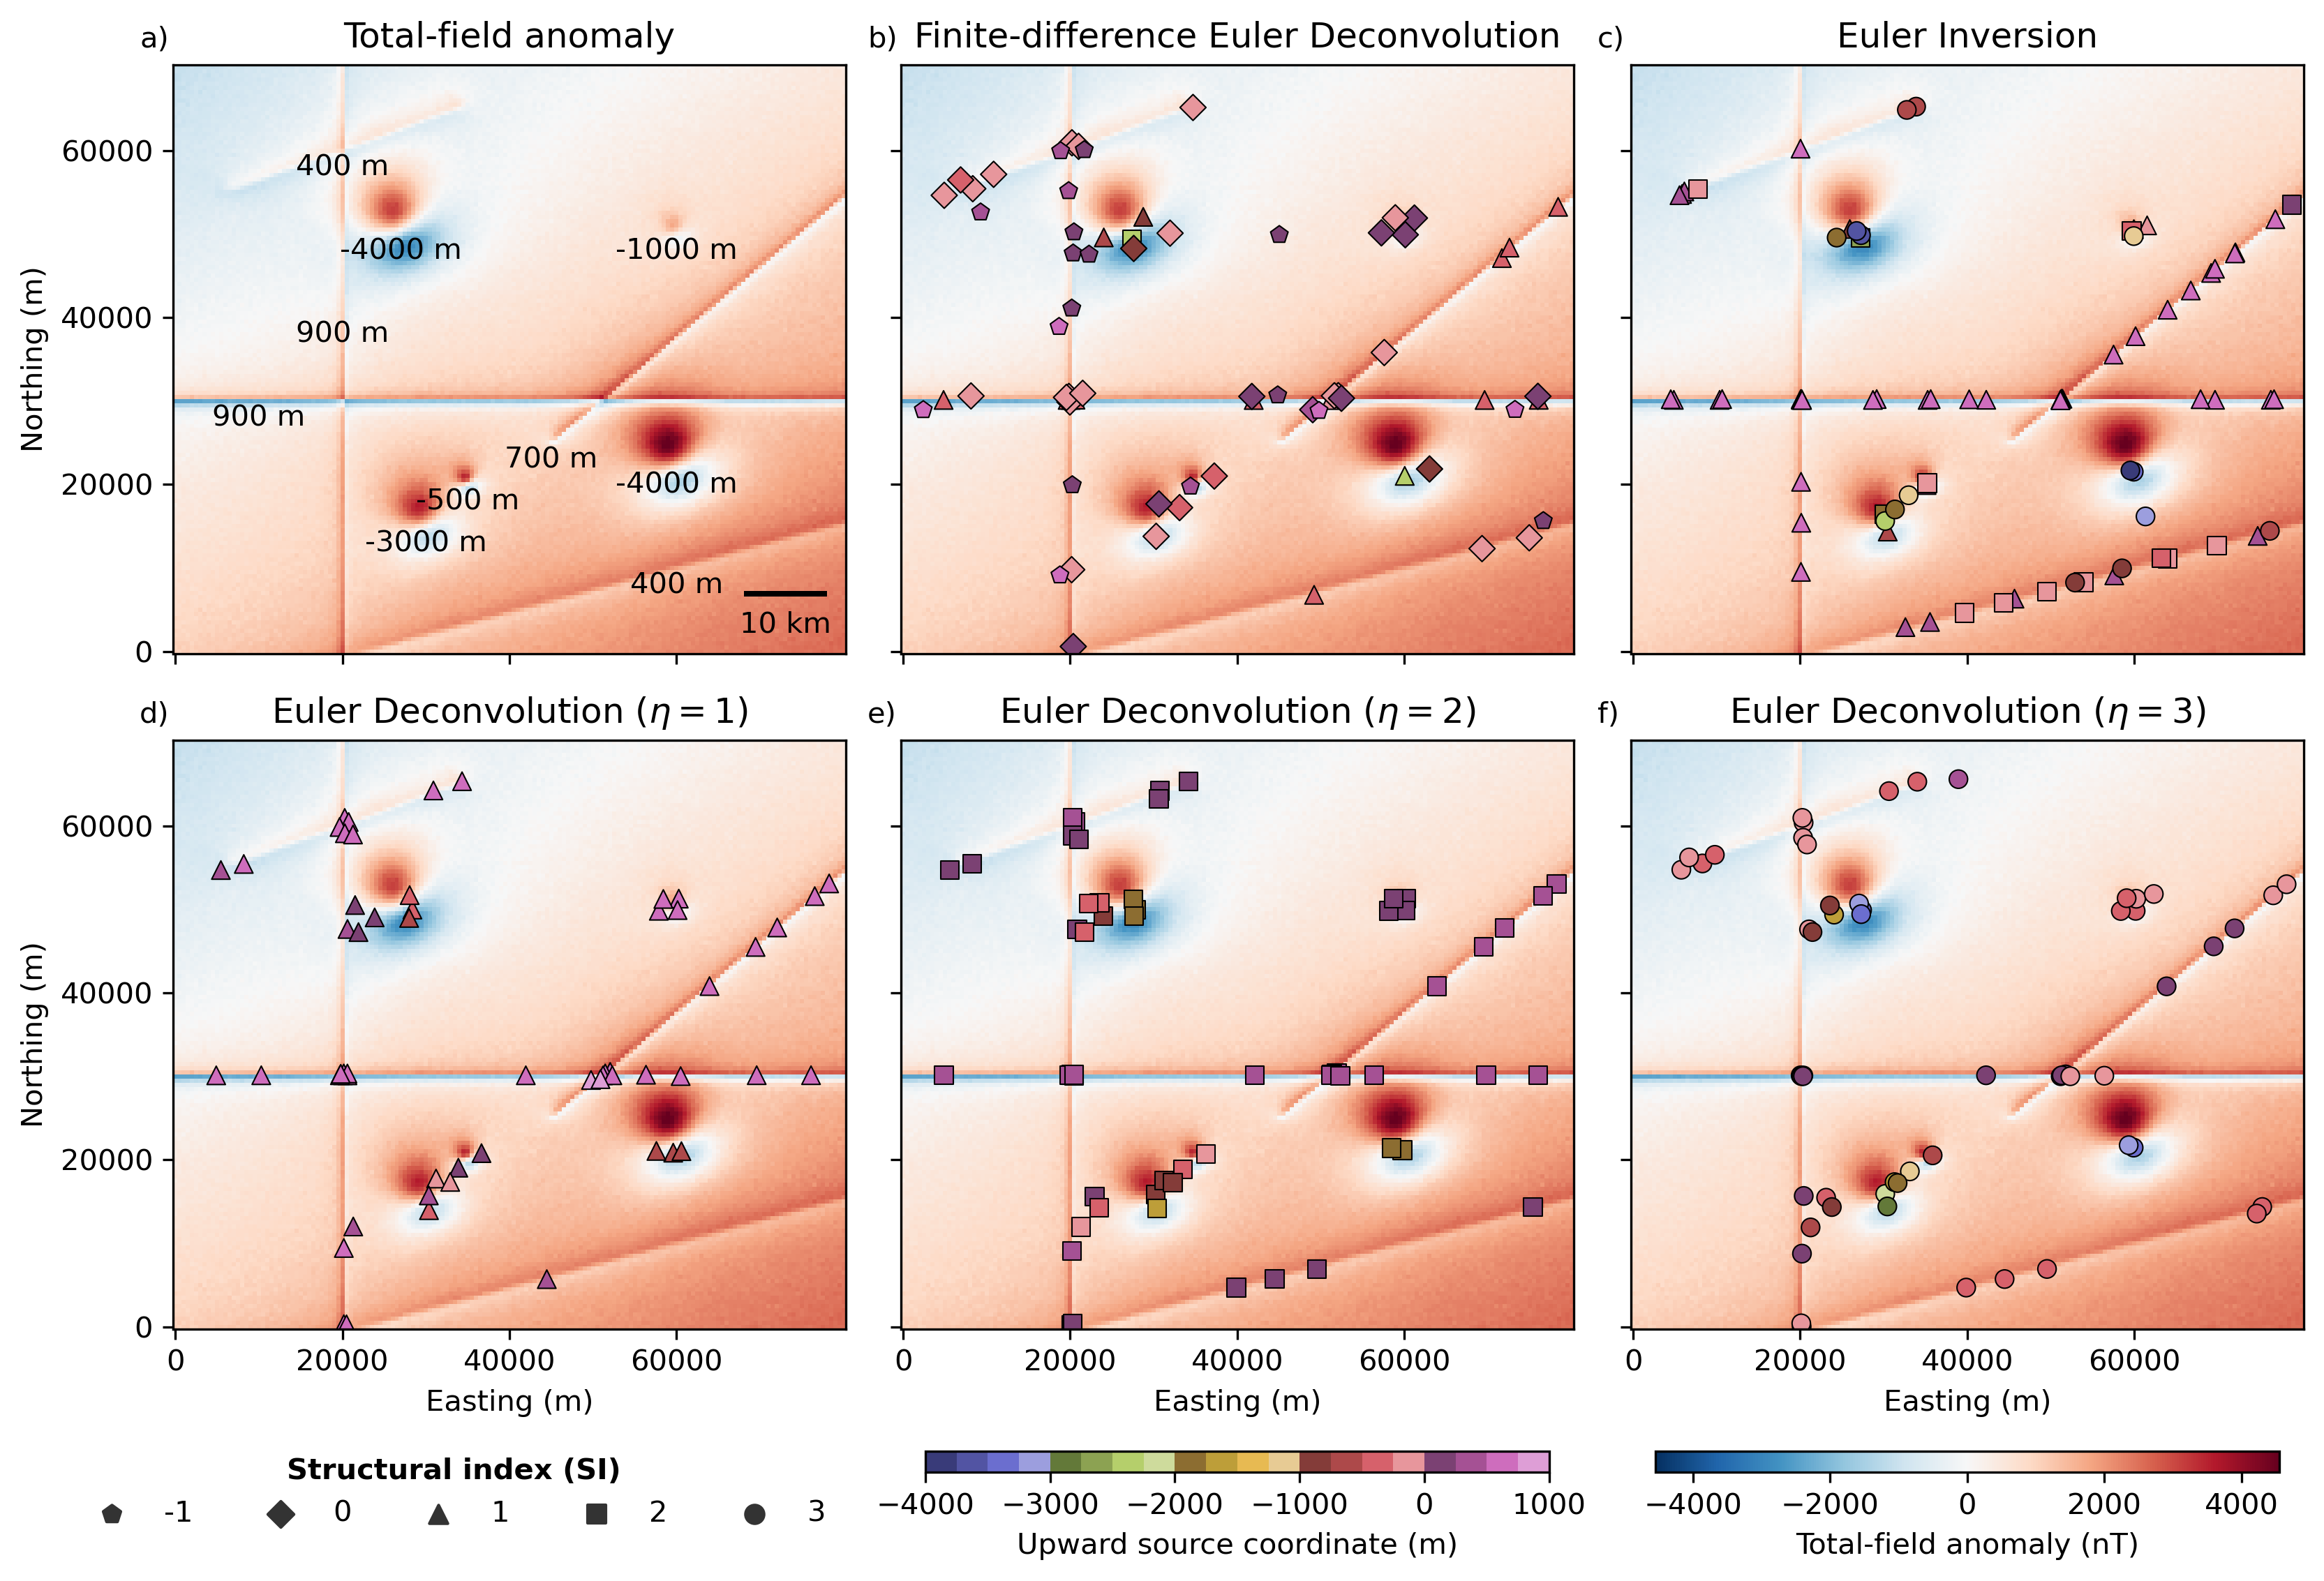
\includegraphics[width=1\linewidth]{euler-inversion/figures/synthetic-windows.png}
\caption{
    Data and results from the synthetic data test using the moving window
    scheme (Algorithm~\ref{alg:window}).
    a) Noise-corrupted total-field magnetic anomaly generated from
    \SynWinNSources{} sources with overlapping signals, including dykes and
    dipoles. The true upward coordinate $z_o$ of each source is shown next to
    their respective anomalies.
    b-f) The estimated source locations from finite-difference Euler
    deconvolution, Euler inversion, Euler deconvolution ($\eta=1$), Euler
    deconvolution ($\eta=2$), and Euler deconvolution ($\eta=3$), respectively.
    The total-field anomaly is shown in the background for reference.
    The structural index of the solutions are represented by pentagons
    ($\eta=-1$),  diamonds ($\eta=0$),  triangles ($\eta=1$),  squares
    ($\eta=2$), and circles ($\eta=3$).
    For finite-difference Euler deconvolution (b), the structural index symbol
    is that of the closest integer to the estimated value.
    The color of each symbol represents the estimated upward coordinate $z_o$.
    The window size used was \SynWinWindowSize{} and the step between windows
    was \SynWinWindowStep{}.
}
\label{fig:windows}
\end{figure}

To simulate a more realistic dataset, we created a model composed of
\SynWinNSources{} sources combining dipoles at various locations and depths and
vertical dykes at various orientations.
All sources had induced magnetisation in the direction of the regional field
with a inclination of \SynWinInc{} and declination of \SynWinDec{}.
The total-field anomaly of the model was calculated on a regular grid with
a spacing of \SynWinSpacing{} and at a constant height of \SynWinHeight{}.
We added to the data a base level of \SynWinBase{}, pseudo-random Gaussian
noise with \qty{0}{\nano\tesla} and \SynWinNoise{} standard deviation, and
a regional field composed of a first-degree polynomial with angular
coefficients of \SynWinRegionalE{} in the eastward and \SynWinRegionalN{} in
the northward directions.
The noise-corrupted total-field anomaly data are shown in
Figure~\ref{fig:windows}a.

To the dataset, we applied the moving window Euler inversion method
(Algorithm~\ref{alg:window} and Algorithm~\ref{alg:si} with
$\eta_{min}=\DefaultSIMin$ and $\eta_{max}=\DefaultSIMax$), the
finite-difference Euler deconvolution method
of \citet{Gerovska2005}, and standard Euler deconvolution (using structural
indices 1, 2, and 3).
Euler inversion was performed with data weights of \DefaultWeightsF{} for the
total-field anomaly, \DefaultWeightsE{} for the eastward derivative,
\DefaultWeightsN{} for the northward derivative, and \DefaultWeightsU{} for the
upward derivative.
All three methods used the same moving window procedure described in
Algorithm~\ref{alg:window} for the sake of comparison.
The windows had a size of \SynWinWindowSize{} and were moved by
\SynWinWindowStep{} at a time.
The ratio of estimates kept to form the final solution was
$\gamma=\SynWinKeepED$ for Euler deconvolution, $\gamma=\SynWinKeepFD$ for
finite-difference Euler deconvolution, and $\gamma=\SynWinKeepEI$ for Euler
inversion.

Figures~\ref{fig:windows}b-f show the estimated source positions and structural
indices for finite-difference Euler deconvolution, Euler inversion, and Euler
deconvolution with structural indices 1, 2, and 3, respectively.
The finite-difference method estimates a non-integer structural index, as
a result Figure~\ref{fig:windows}b shows the closest integer value to the
actual estimated $\eta$.
The finite-difference Euler deconvolution method underestimates the structural
indices of all sources and, therefore, also underestimates their depths.
The finite-difference method solutions are also more scattered than their Euler
deconvolution and Euler inversion counterparts.
The Euler deconvolution results are closer to the correct depths when the
correct structural index is used.
They present larger dispersion than Euler inversion in areas where the signals
of multiple sources overlap.
With the exception of the deeper dykes in the northwest and southeast and the
small dipole with $z_o=\qty{-500}{\m}$, Euler inversion is able to estimate the
correct structural index for most sources.
The upward coordinate estimates for Euler inversion are also closer than Euler
deconvolution to their true values when the correct structural index was
estimated.
Euler inversion notably estimates an incorrect $\eta$ and $z_o$ for smaller
sources when there is a large amount of interference in the anomalies and for
dykes that are deeper and produce a smoother signal.

It is also notable that there are solutions that outline the simulated dykes
for all three methods.
This seems to be in contradiction of the results presented in
Section~\ref{sec:interf} and the theoretical proof in
\citet{Mushayandebvu2004}, which show that the $x_o$ and $y_o$ coordinates
cannot be estimated for 2D sources.
However, these results are widely known in practice where Euler
deconvolution-based methods are routinely used to map dykes and lineaments.
We believe that this is the effect of high-frequency noise.
The derivatives, which appear in the Jacobian matrix
(Equation~\ref{eq:deconv-system}), will contain this high-frequency noise as
well which is not 2D in nature.
This in turn causes the Hessian matrix (Equation~\ref{eq:deconv-p}) to not be
singular in practice.


\subsection{Aeromagnetic data from Rio de Janeiro}
\label{sec:rio}

\begin{figure}[tb!]
\centering
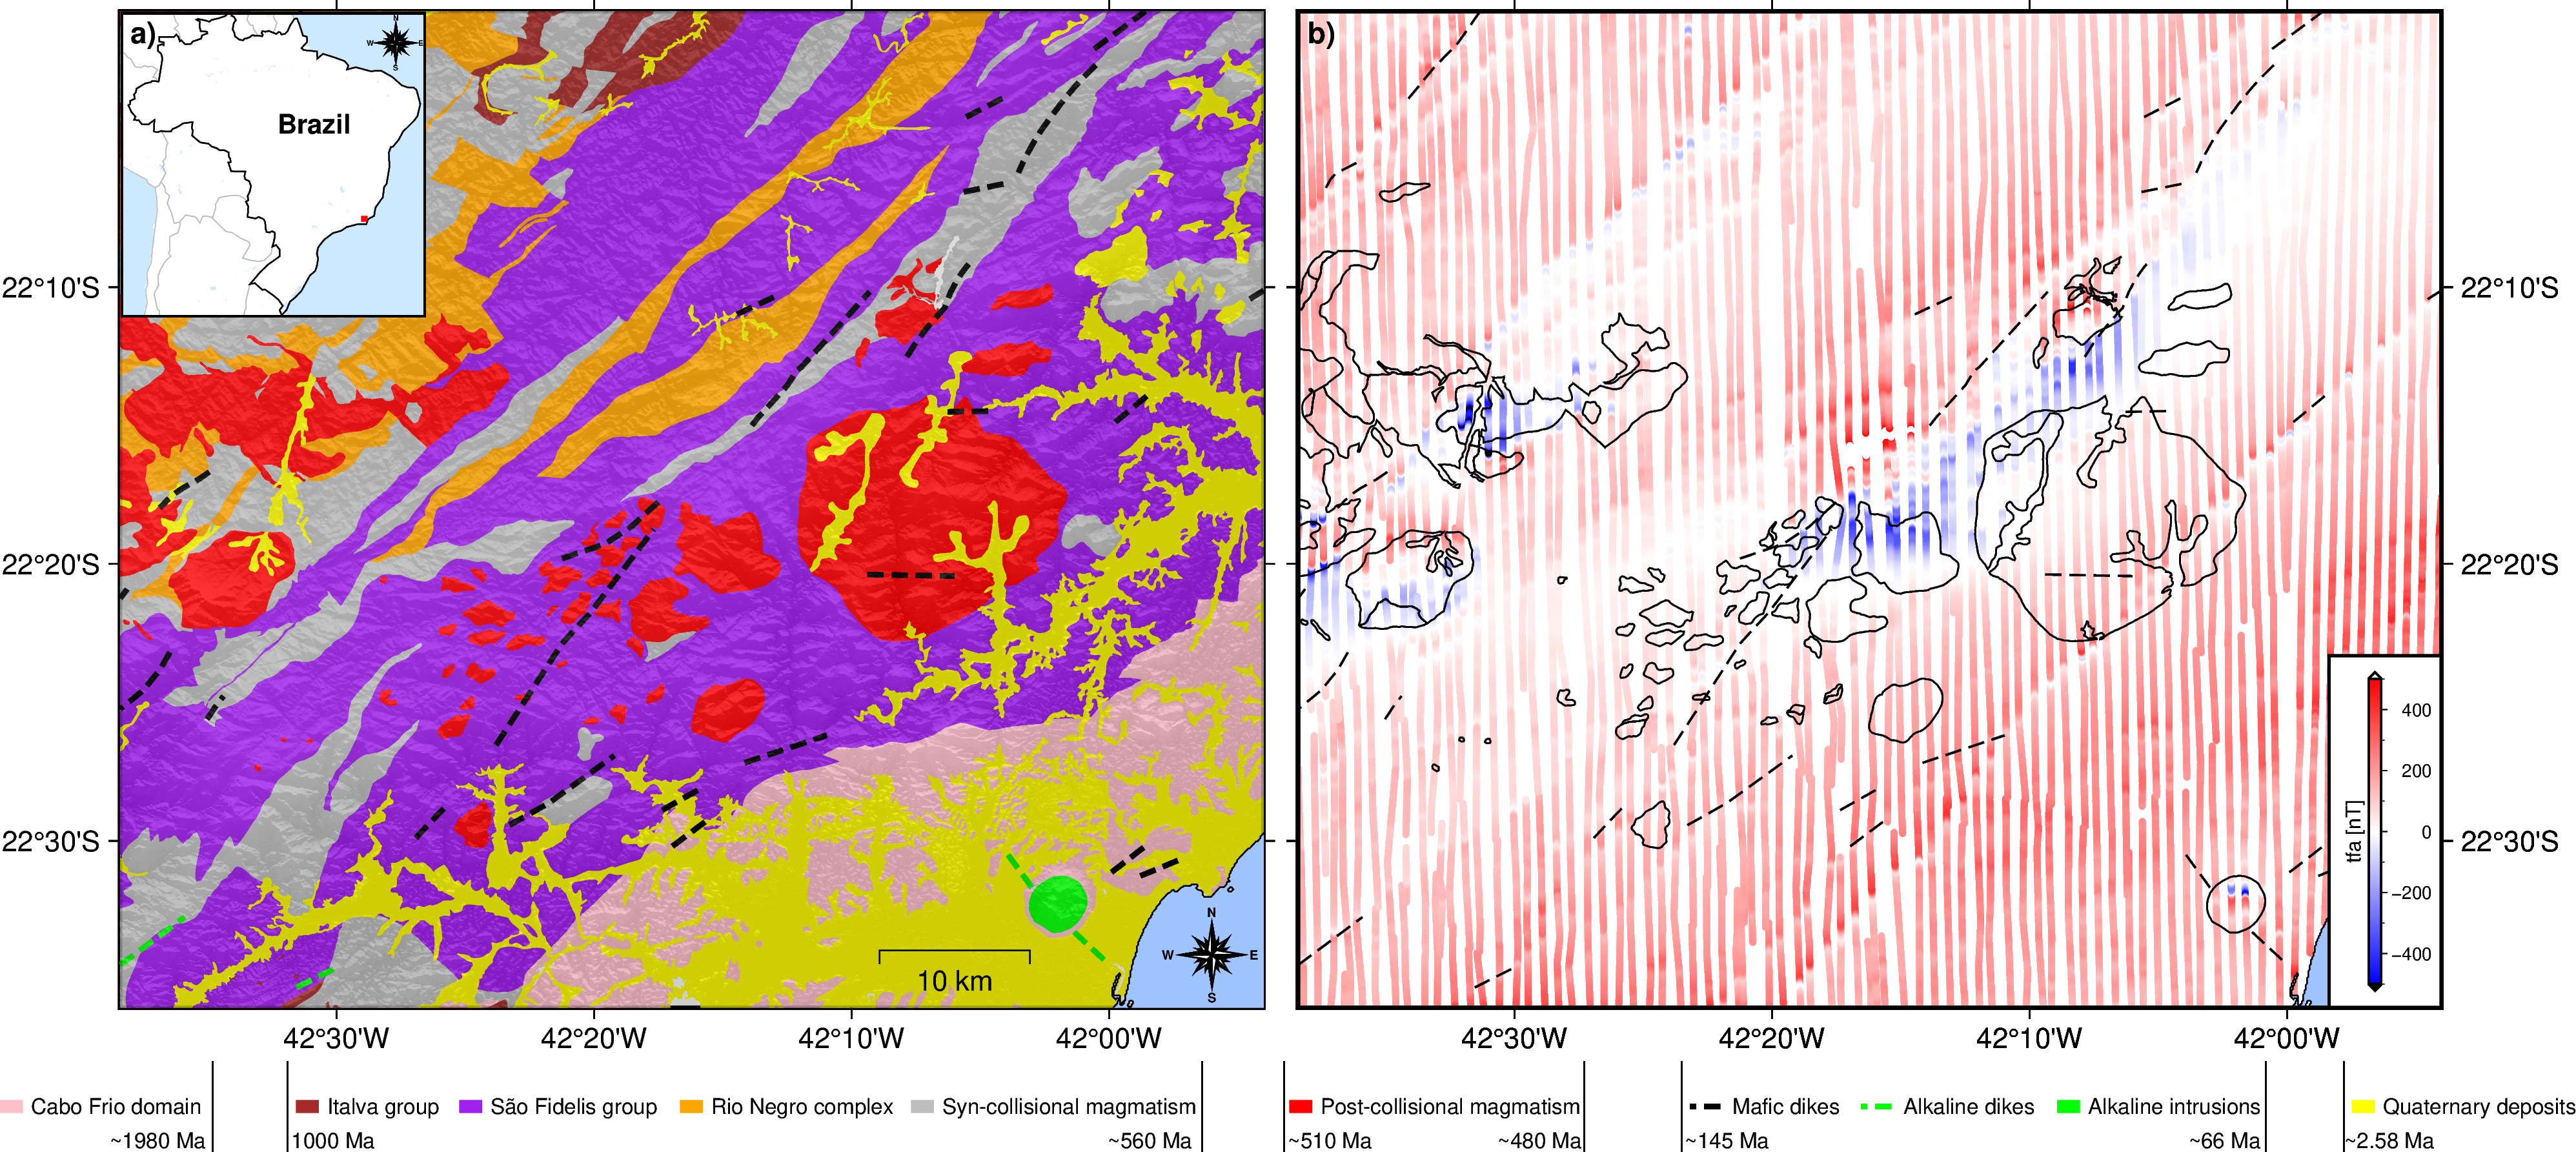
\includegraphics[width=1\linewidth]{euler-inversion/figures/real-data-geology.png}
\caption{
  Geologic map and observed total-field magnetic anomaly data from the west of
  the state of Rio de Janeiro, Brazil.
  a) Simplified geologic map showing the main groups and dykes that outcrop in
  the region.
  In pink is the Cabo Frio domain, dark red is the Italva group, purple is the
  São Fidelis group, orange is the Rio Negro complex, gray is the
  syn-collisional magmatism, red is the post-collisional magmatism, green are
  alkaline intrusions, yellow are the Quaternary deposits, and the dashed lines
  are mafic and alkaline dykes.
  b) The aeromagnetic flight-line data, overlaid by the outlines of the
  post-collisional magmatism and alkaline intrusions (solid black lines) and
  dykes (dashed lines).
  The geologic map was modified from \citet{Heilbron2016} and
  \citet{Dantas2017}.
}
\label{fig:rio_context}
\end{figure}

\begin{figure}[tb!]
\centering
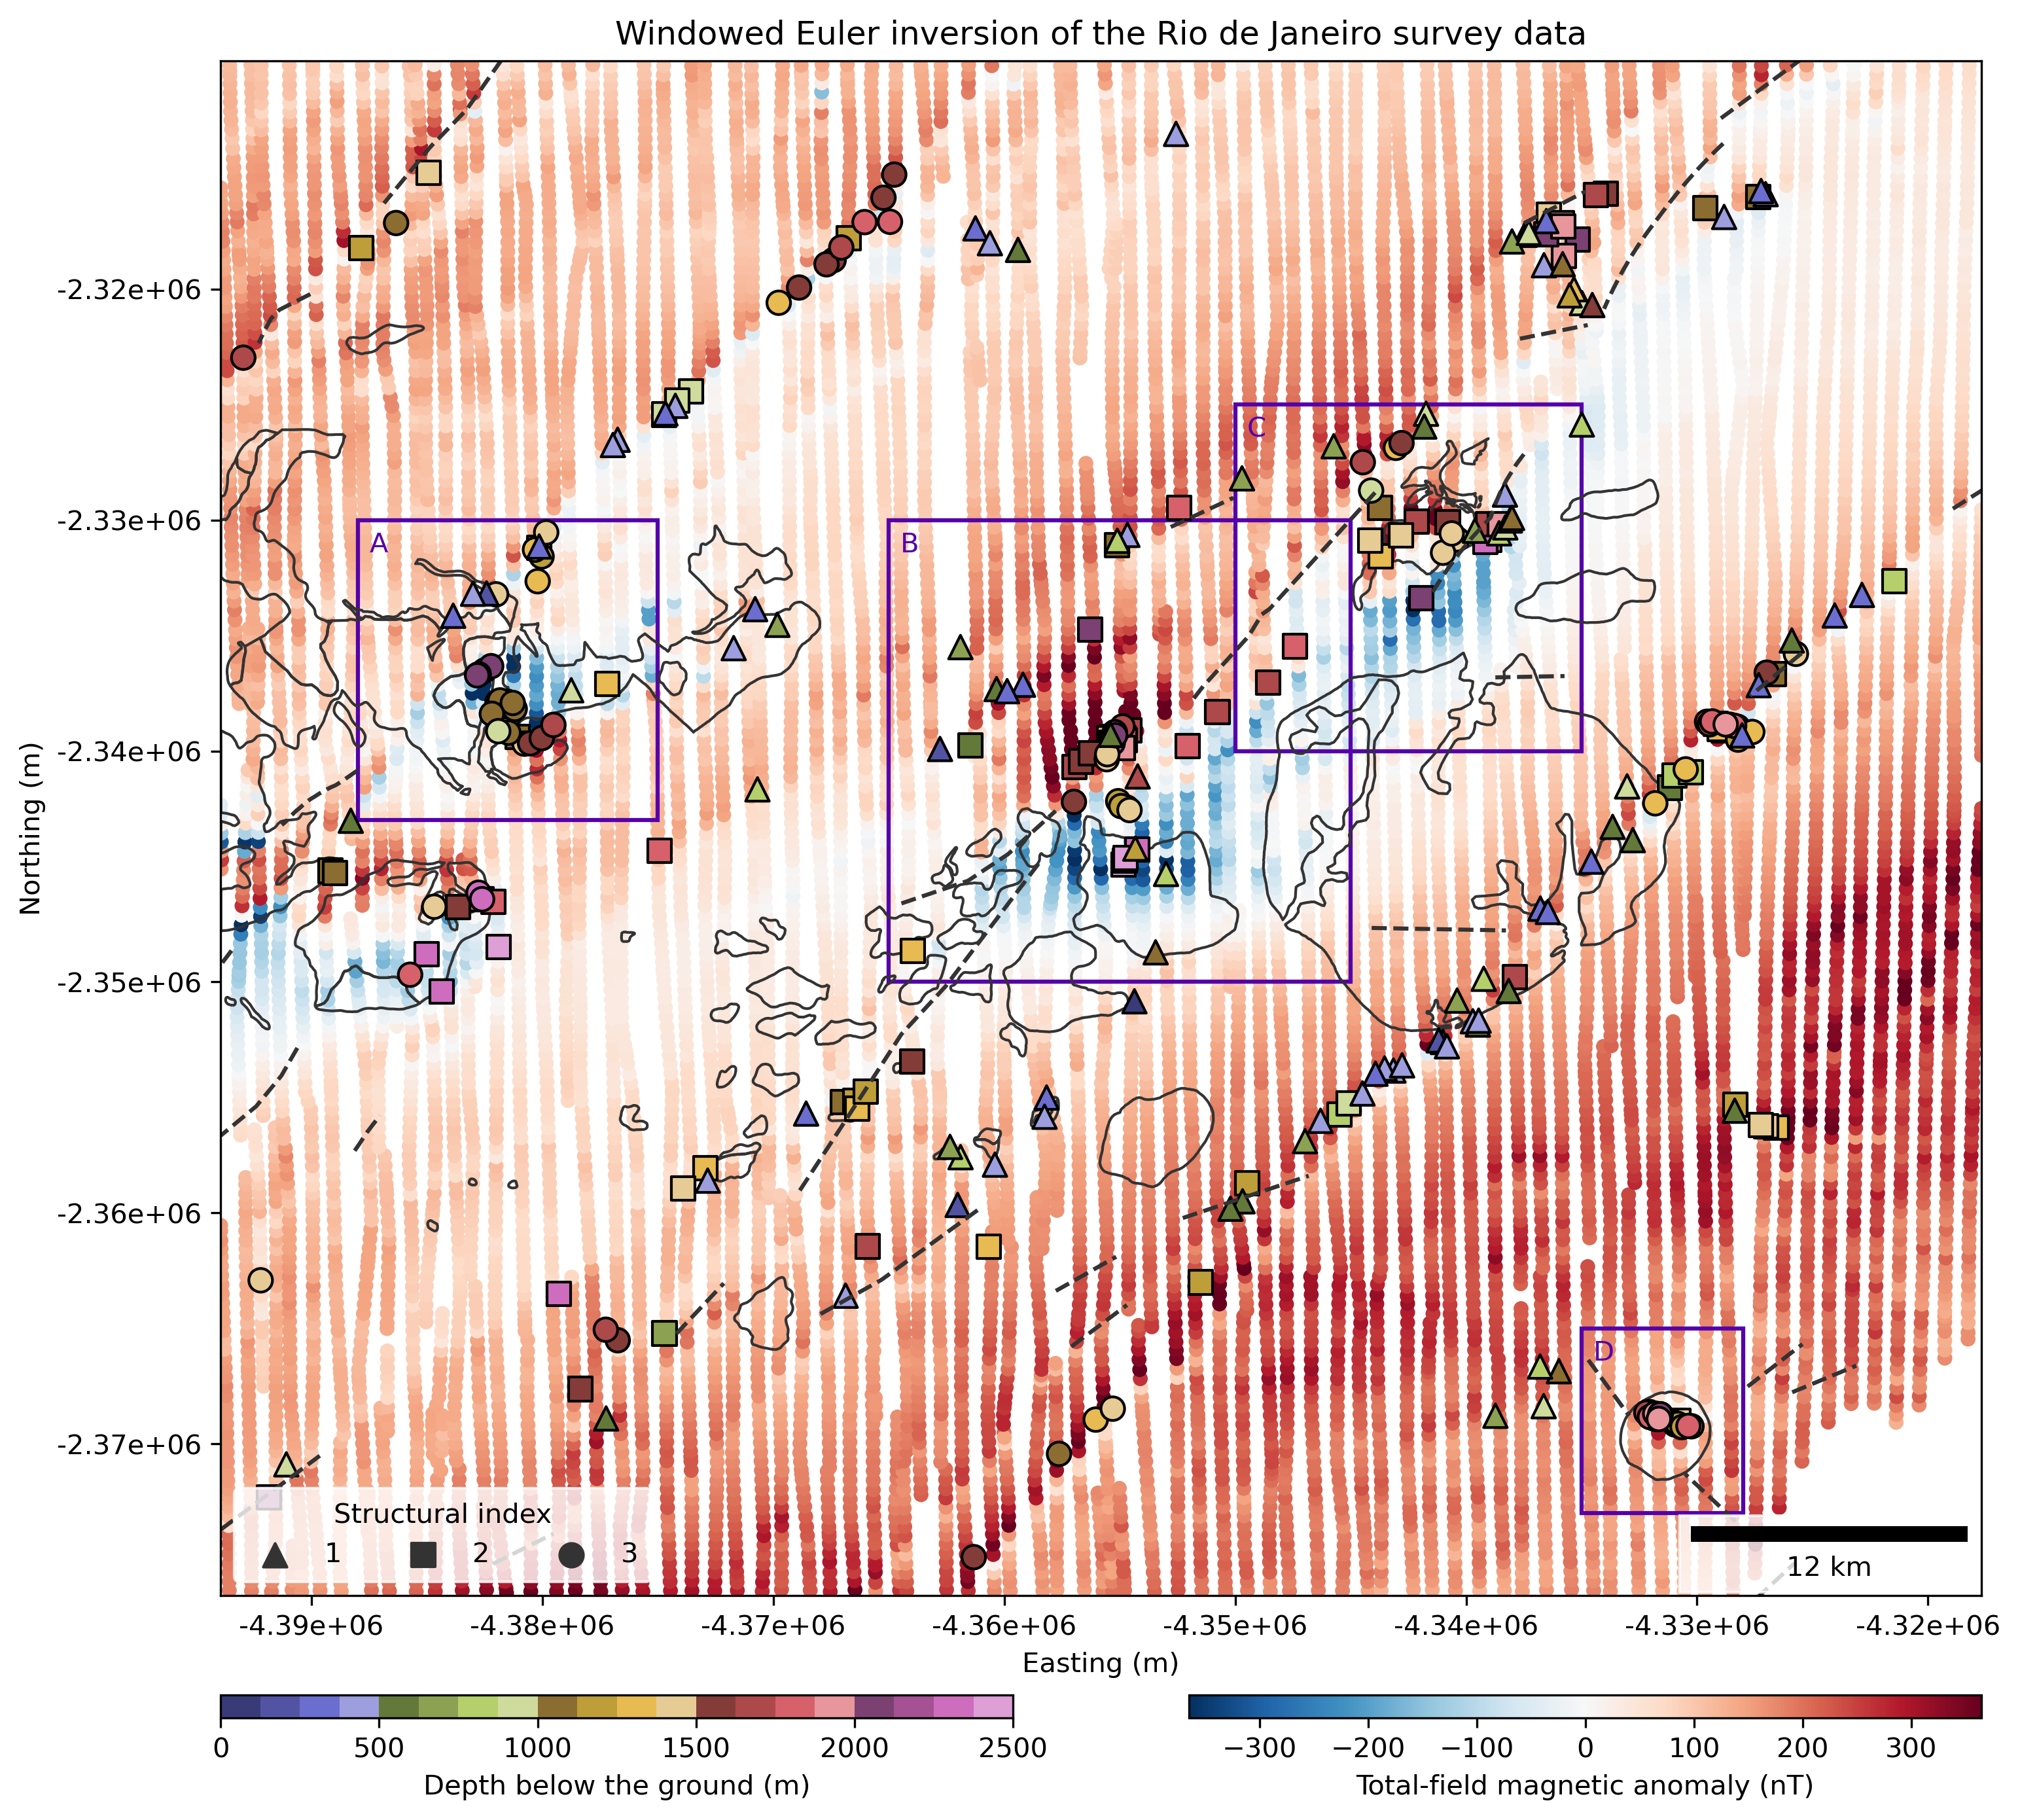
\includegraphics[width=1\linewidth]{euler-inversion/figures/real-data-application.png}
\caption{
    Results of applying Euler inversion with a window size of \RioWindowSize{}
    and a window step of \RioWindowStep{} to the aeromagnetic data from Rio de
    Janeiro, Brazil.
    Estimated source locations and structural indices obtained from Euler
    inversion are shown as triangles ($\eta=1$), squares ($\eta=2$), and
    circles ($\eta=3$).
    The colour of each symbol represents the estimated depth below the surface
    of the Earth (topography).
    Also shown are the total-field anomaly flight-line data, the contours of
    the post-collisional magmatism and alkaline intrusions (solid black lines)
    and dykes (dashed lines).
    The purple squares highlight the A, B, C, and D anomalies that are
    discussed in the text.
}
\label{fig:rio_results}
\end{figure}

\begin{figure}[tb!]
\centering
\includegraphics[width=1\linewidth]{euler-inversion/figures/real-data-application-comparison.png}
\caption{
    Results of applying Euler deconvolution and finite-difference Euler
    deconvolution with a window size of \RioWindowSize{} and a window step of
    \RioWindowStep{} to the aeromagnetic data from Rio de Janeiro, Brazil.
    a-c) Euler deconvolution results with structural index $\eta=1$, $\eta=2$,
    and $\eta=3$, respectively.
    d) Finite-difference Euler deconvolution results.
    The structural index of the solutions are represented by pentagons
    ($\eta=-1$),  diamonds ($\eta=0$),  triangles ($\eta=1$),  squares
    ($\eta=2$), and circles ($\eta=3$).
    For finite-difference Euler deconvolution, the structural index symbol is
    that of the closest integer to the estimated value.
    The colour of each symbol represents the estimated depth below the surface
    of the Earth (topography).
    Also shown are the total-field anomaly flight-line data, the contours of
    the post-collisional magmatism and alkaline intrusions (solid black lines)
    and dykes (dashed lines).
}
\label{fig:rio_comp}
\end{figure}

The geology of Rio de Janeiro state (Southeastern Brazil) consists primarily of
high-grade metamorphic rocks and granitoid magmatism related to the Ribeira
Belt (RB) \citep{Heilbron2020}.
Figure~\ref{fig:rio_context}a shows a simplified geologic map of the area,
which was modified from \citet{Heilbron2016} and \citet{Dantas2017}.
The Ribeira Belt is traditionally interpreted as a thrust
belt formed by diachronous collisions mainly between the São Francisco and
Congo paleocontinents \citep{Heilbron2008, Trouw2000} or by an intracontinental
orogeny \citep[\textit{e.g.}][]{Meira2015, Meira2019}, during the Brasiliano
orogeny. This process culminated in an orogen-parallel, steep strike-slip shear
system \citep{EgydioSilva2005}, which deformed the Paleoproterozoic basement
rocks and reworked the Meso- to Neoproterozoic metasedimentary units (for
example, the Italva and São Fidelis groups) and syn-orogenic granitoid plutons
(for example, the Rio Negro complex) which formed during the orogeny
\citep{Heilbron2003, Heilbron2020}.
These tectonic events imprinted a distinct NE-ENE-trending structural pattern
onto these rocks.

The late Neoproterozoic to Cambrian period witnessed post-orogenic magmatism
\citep[\textit{e.g.,}][]{Valeriano2011}, marking the final stages of the West
Gondwana amalgamation. After this, the region remained tectonically quiescent
until the Lower Cretaceous, when reactivation occurred with the emplacement of
the NE-trending Serra do Mar mafic dyke swarm, preceding the break-up of West
Gondwana and the opening of the South Atlantic Ocean \citep{Almeida2013}.
Lastly, thermal anomalies in the region during the Upper Cretaceous to
Paleocene period led to the emplacement of alkaline complexes and dykes
\citep{Thompson1998}.
The geological complexity of the Ribeira Belt, marked by the interplay of
diverse tectonic regimes and magmatic events (Figure~\ref{fig:rio_context}a),
makes the Rio de Janeiro region an ideal test case for Euler inversion.

We used aeromagnetic data from the state of Rio de Janeiro which are
distributed by the Serviço Geológico do Brasil
(\url{https://geosgb.sgb.gov.br}). The data were collected in two phases:
Subarea 1 was surveyed between March 25 and May 27, 1978, using an Islander
aircraft (PT-KRP), while Subarea 2 was surveyed between April 6 and
July 19, 1978, using a Bandeirante aircraft (PT-GKJ), both funded by the
Brazilian government. As shown in Figure~\ref{fig:rio_context}b, the survey
followed a pattern of north-south flight lines spaced approximately
\qty{1}{\km} apart, with east-west tie lines.
Data were recorded at 100-meter intervals using a Geometrics G-803
magnetometer. Some of the notable features of the data are the NE-SW linear
features (interpreted here as dykes), which coincide with known dyke outcrops,
and complex dipolar anomalies which coincide with some of the post-collisional
magmatism and alkaline intrusions. A subset of \RioNData{} data points were
used in our analysis.

The data were not interpolated on a regular grid to avoid any smoothing effects
that the interpolation might have on the linear features. This could result in
an over-estimation of their depth, as discussed in Section~\ref{sec:windows}.
Instead, we used the gradient-boosted equivalent sources method of
\citet{Soler2021} to fit a model to the observed line data.
We then used the model to make predictions of the three spatial derivatives at
the original measurement locations by a central-difference method with
a coordinate shift of \RioDerivSpacing{}. Further details about the data
processing can be found in the source code archive that accompanies this
article \url{https://doi.org/\ArchiveDOI} \citep{figshare}.

We performed the moving-window Euler inversion (Algorithm~\ref{alg:window} and
Algorithm~\ref{alg:si} with $\eta_{min}=\RioSIMin$ and
$\eta_{max}=\RioSIMax$) on the observed total-field anomaly line data using
windows of size of \RioWindowSize{} which were moved \RioWindowStep{} at
a time.
The proportion of solutions kept was $\gamma=0.15$.
The inversion was performed with data weights of \RioWeightsF{} for the
total-field anomaly, \RioWeightsE{} for the eastward derivative, \RioWeightsN{}
for the northward derivative, and \RioWeightsU{} for the upward derivative.
To aid in the geological interpretation of the results, we converted the
estimated upward source coordinates $z_o$ to depths below the surface of the
Earth. We did so by subtracting the estimated $z_o$ from the interpolated
topographic height of the Shuttle Radar Topography Mission
\citep[SRTM;][]{SRTM}. The estimated positions and structural indices are shown
in Figure~\ref{fig:rio_results}.
We also performed Euler deconvolution with structural indices one, two, and
three, as well as finite-difference Euler deconvolution on the same dataset
using the same window size and window step for the sake of consistency.
These results are shown in Figure~\ref{fig:rio_comp}.

The Euler inversion estimated source positions shown in
Figure~\ref{fig:rio_results} highlight the NE-SW lineaments as well as some of
the more dipolar anomalies.
The lineaments are estimated with a mix of $\eta=1$, $\eta=2$, and $\eta=3$.
The southernmost lineament is mostly estimated with $\eta=1$ and depths
suggesting that it does not outcrop in its southernmost parts (depths of
\qtyrange{400}{600}{\m}), which is consistent with the geologic information in
Figure~\ref{fig:rio_context}a. The southernmost part of this lineament, in
particular, has an estimated $\eta=3$, which is known to happen for deeper
dykes in our synthetic data tests (Section~\ref{sec:windows}). Conversely, the
northernmost part of the lineament has a larger prevalence of $\eta=1$ with
shallower depths which coincide with a known dyke outcrop.
Other known dyke outcrops coincide with estimated sources with $\eta=1$,
however their depths range from \qtyrange{100}{300}{\m}. This may be caused by
an excess of smoothing in the vertical derivative or effects of noise in the
estimated coordinates. The lineaments in the northwestern part of the region
are also highlighted by estimated sources.
However, their structural indices are a mix of $\eta=2$ and $\eta=3$,
suggesting deeper sources. This is inline with the geologic information, which
includes no outcrops of linear structures in the area.

The dipolar anomalies are associated with post-collisional and alkaline
intrusions, many of which are also cut by known outcropping dykes or have known
dykes with magnetic signals that significantly overlap with the dipolar
anomalies. The Euler inversion estimated structural indices for them range from
$\eta=2$ to $\eta=3$. We have highlighted four dipolar anomalies, marked as A,
B, C, and D in Figure~\ref{fig:rio_results}, to aid in our discussion.

\begin{itemize}
\item \textbf{Anomaly A:} Has a reversed polarity and linear feature to its
    north that is not associated with any known dyke outcrop. The linear
    feature is highlighted by Euler inversion estimates with $\eta=1$ and depth
    of \qtyrange{300}{400}{\m}, which can be interpreted as a non-outcropping
    dyke. The dipolar anomaly itself has Euler inversion solutions with
    $\eta=3$ and depth of \qtyrange{1000}{2000}{\m}.
    The solutions in the centre of the anomaly present a shallower depth than
    the solutions to the north and south of the anomaly centre. From the
    results on synthetic data in Section~\ref{sec:windows}, we can interpret
    the depth range to be caused by the moving window procedure and the effect
    of interfering sources. The depth to the centre of the anomaly source is
    likely close to \qty{1000}{\m}.

\item \textbf{Anomaly B:} The dipolar anomaly is likely associated with
    a non-outcropping portion of the post-collisional magmatism. The anomaly is
    cut by several NE-SW linear features, some of which overlap with known dyke
    outcrops. The linear feature to the north is associated with Euler
    inversion results with $\eta=1$ and depths ranging from
    \qtyrange{300}{600}{\m}, suggesting a non-outcropping dyke. At the centre
    of the anomaly are Euler inversion estimates with $\eta=3$ and depth
    estimate of approximately \qty{1400}{\m}. The Euler inversion solutions
    surrounding these central solutions are likely caused by interference from
    other sources.

\item \textbf{Anomaly C:} A dipolar anomaly associated with an outcropping
    portion of the post-collisional magmatism. There is a known outcropping
    dyke to the south of the anomaly, which is associated with Euler inversion
    estimates with $\eta=1$ and depths ranging from \qtyrange{500}{1000}{\m}.
    These depth estimates are likely overestimated because of the interference
    of the dipolar anomaly. The main anomaly has Euler inversion solutions with
    $\eta=2$ and $\eta=3$ and depths varying from \qtyrange{1400}{1800}{\m}.
    There is no clear indication of which of these estimates is more reliable.

\item \textbf{Anomaly D:} A small dipolar anomaly associated with an
    outcropping alkaline intrusion. The Euler inversion estimates have $\eta=3$
    and depths \qtyrange{1700}{2000}{\m}. There are known outcropping dykes
    around the main intrusion but they have no discernible magnetic anomalies
    and no Euler inversion solutions associated with them.
\end{itemize}

Overall, the Euler inversion solutions in Figure~\ref{fig:rio_results} are
consistent with the known geology in Figure~\ref{fig:rio_context}a.
The main linear features are mostly associated with Euler inversion estimates
with $\eta=1$ and shallow depths, particularly where known dyke outcrops are
located.
Deeper linear features are estimated with $\eta=2$ and $\eta=3$, which is
consistent with the synthetic data results (Section~\ref{sec:windows}).
The dipolar anomalies have consistent Euler inversion estimates with $\eta=3$
when they are well isolated from interfering sources.
Otherwise, they are estimated with a mix of structural indices and depths, as
was demonstrated in Section~\ref{sec:windows}.

When compared to the Euler deconvolution and finite-difference Euler
deconvolution results (Figure~\ref{fig:rio_comp}), the Euler inversion results
are less dispersed and better delinear the linear features present in the data.
The structural index results from finite-difference Euler deconvolution
(Figure~\ref{fig:rio_comp}d) are underestimated, with most values of $\eta$
being less than one, which is not in accordance with the geology of the area.

%%%%%%%%%%%%%%%%%%%%%%%%%%%%%%%%%%%%%%%%%%%%%%%%%%%%%%%%%%%%%%%%%%%%%%%%%%%%%%%
\section{Conclusion}

Euler deconvolution is a widely used method for locating the sources of
potential-field data.
It has its limitations in real-world scenarios due to its dependence on the
chosen value of the structural index $\eta$ and its sensitivity to
high-frequency noise and signal overlap from interfering sources.
We have developed a new method to solve Euler's homogeneity equation for the
source position, base level, and integer structural index, which we call
\textit{Euler inversion}.
Unlike Euler deconvolution, Euler inversion is also able to estimate the
predicted field and its spatial derivatives, as well as assign different
weights to each type of data.
Our method can be applied to gridded and non-gridded data, which can
be useful to limit the effects of smoothing from interpolation in the final
results when the original data have large spacing between flight lines.
The Euler inversion algorithm is computationally efficient because most of the
large matrices involved in the computations are diagonal or block-diagonal.
We found that, in practice, the computation time of Euler inversion and Euler
deconvolution are on the same order of magnitude.

Tests on synthetic data show that Euler inversion outperforms Euler
deconvolution and finite-dif\-fer\-ence Euler deconvolution (a variant that
estimates $\eta$ but does not rely on second-order derivatives) in terms of
robustness to random noise and interfering sources inside the data window.
Our tests also show that the estimated $z_o$ coordinate is correlated with the
structural index, as is the case for Euler deconvolution.
We have also found that the data misfit from Euler inversion is minimal when
the integer structural index used is equal or close to the true one for
idealized sources.
This led us to develop an algorithm for estimating the best integer structural
index based on the data misfit.
A test on complex synthetic data from a model of dykes and dipoles with
overlapping signals shows that Euler inversion is able to estimate the
structural index and position of the sources within expected error bounds when
the signal overlap is not larger than the data window.
For deeper dykes in particular, Euler inversion was not able to estimate the
correct $\eta=1$, leading to an overestimation of the depths.

We applied Euler inversion to an aeromagnetic dataset from Rio de Janeiro,
Brazil, to analyse its performance under real-world scenarios.
Euler inversion was able to locate the NE-SW linear features in the data with
an $\eta=1$ which are associated with known dyke outcrops.
For the deeper linear features, Euler inversion was not able to estimate the
correct $\eta=1$.
Some of the dipolar anomalies present in the data were picked out with
$\eta=3$, while the sources with a large signal overlap with other features
provided a mix of $\eta=2$ and $\eta=3$.
These results are consistent with the synthetic data tests and show the
benefits and limitations of the proposed method.

Euler inversion outperforms Euler deconvolution and finite-difference Euler
deconvolution in most cases.
Its reduced sensitivity to noise and interfering sources, in particular,
may prove beneficial for magnetic microscopy studies, in which high-frequency
noise and interference from multiple dipolar sources are a significant hurdle
\citep{Souza-Junior2024}.
However, it still suffers from some of the same limitations.
While Euler inversion is less sensitive to signal overlap, it still fails to
correctly estimate the position and structural index when the overlap is large.
The windowing procedure still generates a large amount of spurious solutions
which need to be filtered out.
This could be improved with techniques like the source detection method
proposed by \citet{Castro2020}, for example.
Euler inversion can also be coupled with other inverse problems by following
our methodology to add Euler's equation as a non-linear constraint.
This could help with issues of non-uniqueness and stability in traditional 3D
inverse problems in potential-field methods.

As is the case with other Euler deconvolution-based methods, Euler inversion
also suffers from instability when sources are 2D \citep{Mushayandebvu2004}
and a lack of support for sources that are defined by multiple points, for
example steps which have a top and bottom \citep{Gerovska2010}.
The issue of instability was evident in our synthetic data tests which
simulated dykes and did not contaminate the data with random noise.
However, both in the synthetic data tests with noise and the real data
application, this did not appear to be a significant issue.
In both cases, Euler inversion was better at outlining the 2D sources than
Euler deconvolution.
Nonetheless, it would be worthwhile to investigate this issue further and
explore the use of regularization and an adaptation of the method of
\citet{Mushayandebvu2004} to the Euler inversion mathematical formulation.
A thorough comparison of Euler inversion with the Similarity Transform-based
methods, like \citet{Gerovska2010}, would also be worth pursuing.
Euler inversion could complement such methods, which often require gridded
data, in cases where data are of poor quality or flight-line spacing is large.


%%%%%%%%%%%%%%%%%%%%%%%%%%%%%%%%%%%%%%%%%%%%%%%%%%%%%%%%%%%%%%%%%%%%%%%%%%%%%%%
\section*{Data availability statement}

The Python source code and data that were used to produce all results and
figures presented here are available at
\url{https://github.com/\GitHubRepository}
and \url{https://doi.org/\ArchiveDOI} \citep{figshare}
under the CC-BY license and the MIT license.
This study made use of the following open-source scientific software:
matplotlib \citep{Hunter2007} and PyGMT \citep{pygmt} for generating figures
and maps,
Numpy \citep{numpy} and Scipy \citep{scipy} for linear algebra,
Pandas for manipulating tabular data \citep{McKinney2010,pandas},
GeoPandas for reading and plotting shapefiles \citep{geopandas},
pyproj for data projection \citep{pyproj},
xarray \citep{xarray} for working with gridded data,
Verde \citep{verde2018} for moving windows and interpolation,
and Harmonica \citep{harmonica} for potential-field data processing and
modeling.
The aeromagnetic and geologic data are available from Serviço Geológico do
Brasil (\url{https://geosgb.sgb.gov.br}) under a CC-BY-NC license.
The magnetic data are part of survey 1038 ``Projeto Aerogeofísico São Paulo --
Rio de Janeiro''.
Both are also available in our source code and data archive \citep{figshare}.


%%%%%%%%%%%%%%%%%%%%%%%%%%%%%%%%%%%%%%%%%%%%%%%%%%%%%%%%%%%%%%%%%%%%%%%%%%%%%%%
\section*{Acknowledgements}

We are indebted to the developers and maintainers of the open-source software
without which this work would not have been possible.
We thank Dr. Valéria C. F. Barbosa for many insightful discussions over the
years which helped shape our research.
We are grateful to editor Dr. Kosuke Heki and reviewers Dr. Alan B. Reid and
Dr. Saulo Oliveira for their constructive comments.
LU would like to thank Prof. Spiros Pagiatakis for being an incredible
instructor and teaching him the mathematics which formed the foundations of
this work during his undergraduate exchange at York University.
LU was supported in part by start-up grant PRPI 22.1.09345.01.2 from
Universidade de São Paulo.
GFSJ was supported by scholarship 2021/08379-5 from the Fundação de Amparo
à Pesquisa do Estado de São Paulo (FAPESP).
The opinions, hypotheses, and conclusions or recommendations expressed in this
material are the responsibility of the authors and do not necessarily reflect
the views of FAPESP.

\section*{CRediT author contributions}

\textbf{Leonardo Uieda:} Conceptualisation, Data curation, Formal analysis,
Investigation, Methodology, Pro\-ject administration, Resources, Software,
Supervision, Visualisation, Writing – original draft.

\noindent
\textbf{Gelson Ferreira Souza-Junior:} Data curation, Formal analysis,
Resources, Software, Visualisation, Writing - original draft, Writing - review
\& editing.

\noindent
\textbf{India Uppal:} Data curation, Formal analysis, Investigation, Software,
Writing - review \& editing.

\noindent
\textbf{Vanderlei Coelho Oliveira Jr.:} Conceptualisation, Methodology, Writing
- review \& editing.

\endgroup

%==============================================================================
% \bookmarksetup{startatroot}
\chapter{Conclusion}

Bla.


%%%%%%%%%%%%%%%%%%%%%%%%%%%%%%%%%%%%%%%%%%%%%%%%%%%%%%%%%%%%%%%%%%%%%%%%%%%%%%%
\bibliographystyle{apalike-doi}
\bibliography{references}

\end{document}
